% arara: pdflatex: { synctex: yes }
% arara: makeindex: { style: ctuthesis }
% arara: bibtex

% The class takes all the key=value arguments that \ctusetup does,
% and a couple more: draft and oneside
\documentclass[twoside]{template/ctuthesis}



% Bibliography
\usepackage[backend=biber, style=numeric]{biblatex}
\addbibresource{ctutest.bib}

% \DeclareSourcemap{
%   \maps[datatype=bibtex]{
%     \map[overwrite]{
%       \step[fieldsource=keywords, match=\regexp{\A.+\Z}, final]
%       \step[fieldset=keywords, fieldvalue={,hit}, append]
%     }
%     \map{
%       \step[fieldset=keywords, fieldvalue={hit}]
%     }
%   }
% }

% \DeclareSourcemap{
%   \maps[datatype=bibtex]{
%     \map{
%       \step[fieldsource=url, match=\regexp{github.com}]
%     %   \step[fieldset=keywords, fieldvalue={$1}]
%     }
%   }
% }

% \printbibliography[heading=subbibliography, keyword=github.com, title={Github repositories}]


\ctusetup{
	preprint = \ctuverlog,
	mainlanguage = english,
	otherlanguages = {czech},
	title-czech = {},
	title-english = {Bluetooth Low Energy Remote Control of Active Lightning Systems},
	doctype = M,
	faculty = F3,
	department-czech = {Katedra řídicí techniky},
	department-english = {Department of Control Engineering},
	author = {Ladislav Štefka},
	supervisor = {Ing. Pavel Píša, Ph.D},
	subfieldofstudy-english = {Cybernetics and Robotics},
	subfieldofstudy-czech = {Kybernetika a Robotika},
	keywords-czech = {},
	day = 1,
	month = ,
	year = 2022,
	specification-file = {},
	front-specification = true,
	ctulstbg = none,
	%monochrome = true,
%	savetoner = true,
	%layout-short = true,
	pkg-hyperref = true,
	pkg-listings = true,
}

\ctuprocess

\addto\ctucaptionsczech{%
	\def\supervisorname{Vedoucí}%
	\def\subfieldofstudyname{Studijní program}%
}

\ctutemplateset{maketitle twocolumn default}{
	\begin{twocolumnfrontmatterpage}
		\ctutemplate{twocolumn.thanks}
		\ctutemplate{twocolumn.declaration}
		\ctutemplate{twocolumn.abstract.in.titlelanguage}
		\ctutemplate{twocolumn.abstract.in.secondlanguage}
		\ctutemplate{twocolumn.tableofcontents}
		\ctutemplate{twocolumn.listoffigures}
	\end{twocolumnfrontmatterpage}
}

% Theorem declarations, this is the reasonable default, anybody can do what they wish.
% If you prefer theorems in italics rather than slanted, use \theoremstyle{plainit}
\theoremstyle{plain}
\newtheorem{theorem}{Theorem}[chapter]
\newtheorem{corollary}[theorem]{Corollary}
\newtheorem{lemma}[theorem]{Lemma}
\newtheorem{proposition}[theorem]{Proposition}

\theoremstyle{definition}
\newtheorem{definition}[theorem]{Definition}
\newtheorem{example}[theorem]{Example}
\newtheorem{conjecture}[theorem]{Conjecture}

\theoremstyle{note}
\newtheorem*{remark*}{Remark}
\newtheorem{remark}[theorem]{Remark}

 \setlength{\parskip}{2ex plus 0.2ex minus 0.2ex}

% Abstract in Czech
\begin{abstract-czech}
  ... 
\end{abstract-czech}

% Abstract in English
\begin{abstract-english}
...
    
\end{abstract-english}

% Acknowledgements / Podekovani
\begin{thanks}
...
\end{thanks}

% Declaration / Prohlaseni
\begin{declaration}
  ...
\end{declaration}

% Only for testing purposes
\listfiles
\usepackage[pagewise]{lineno}
\usepackage{lipsum,blindtext}
\usepackage{mathrsfs} % provides \mathscr used in the ridiculous examples
\usepackage{tabularx, array, booktabs} %notations

\usepackage{siunitx}
\usepackage{textcomp}
\usepackage{caption}
\usepackage{subcaption}
\usepackage{makecell}
\usepackage{multirow}
\usepackage{tabulary}

\usepackage{rotating}



% ADDED: draw shapes 
\usepackage{tikz,siunitx}
\usetikzlibrary{shapes.geometric,shapes.symbols}
\newcommand{\tikzcircle}[2][red,fill=red]{\tikz[baseline=-0.5ex]\draw[#1,radius=#2] (0,0) circle ;}%
\newcommand{\tikzsymbol}[2][circle]{\tikz[baseline=-0.5ex]\node[inner sep=3pt,shape=#1,draw,#2]{};}%

% ADDED: smaller capitals in table
\usepackage{graphicx}
\catcode`\"=13
\def"#1"{\scalebox{0.8}[0.9]{#1}}




\newcommand{\sss}[1]{\scalebox{0.9}[0.9]{#1}}
\RenewDocumentCommand{\_}{}{\scalebox{0.5}[1]{\textunderscore}}

% ADDED: itemize with title 
\newenvironment{titleitemize}[1]{%
    \paragraph{#1}
    \setlength{\parskip}{0pt}
    \begin{itemize}
    \setlength\itemsep{0.15em}}
    {\end{itemize}} 

\newcommand{\todo}[1]{\textcolor{red}{\textbf{TODO: #1}}\PackageWarning{TODO:}{#1!}}

\newcommand{\question}[1]{\textcolor{blue}{\textbf{QUESTION: #1}}\PackageWarning{QUESTION:}{#1!}}

\newcommand{\answer}[1]{\textcolor{magenta}{\textbf{ANSWER: #1}}\PackageWarning{ANSWER:}{#1!}}

\begin{document}


% \maketitle

%!TEX ROOT=ctutest.tex




\chapter{Introduction}
     \todo{HUMAN SAFETY IN LOWLIGHT CONDITIONS}
   
\section{Active Lighting Systems}
   
     \todo{ACTIVE LIGHTING SYSTEM ADVANTAGES - reuse SCILIF state of art}
     
     SunFibre Wearable Active Lighting Technology is an optic fibre lighting system that increases visibility in darkness or lowlight conditions. Unlike retroreflective safety elements, it emits light through optic fibres encased in a textile coating, ensuring active protection. Side-emitting optic fibres provide visibility in all directions up to a distance of 3 kilometres. The properties of the textile coated optic fibre allow easy sewing into textile products and guaranteed mechanical durability and washability. The system is easy to operate and recharge
     
     
     \todo{}
    

\section{Remote Control of Lighting Systems}
    
  
% %!TEX ROOT=ctutest.tex
\chapter{Stávající řešení a přínos práce}

\section{Situace na trhu}
    V současné době se již existujících systémů pro monitorování vibrací na trhu objevuje hned několik. Obecně se od sebe liší především oblastí použití, komplexností, přesností monitorování a hlavně konektivitou. Rozdílné požadavky zákazníků poté rozhodují o konkrétním výběru. Ačkoliv obecnější informace a statistiky o rozložení trhu se mi nalézt nepodařily, v této kapitole bych představil a porovnal několik nejmodernějších existujících řešení.  
    
    \subsection{ABB WiMon Condition Monitoring System}
        ABB je švédsko-švýcarská firma, jeden z největších technologických konglomerátů na světě (114. místo v žebříčku Forbes), zabývající se robotizací a digitalizací průmyslu \cite{manufactor:1}. Produkty ABB jsou z dnešního pohledu na Internet věcí poměrně těžkopádné. ABB využívá pro komunikaci WirlessHART, technologii, která není dobře integrovatelná do moderních IoT systémů, a systém je navíc zcela uzavřený, vhodný hlavně jako rozšíření do již existující průmyslové diagnostické infrastruktury využívající systémy ABB. Navíc i přes dobré diagnostické možnosti v softwaru WiMon Data Manager a nastavitelná upozornění pro monitorované veličiny, postrádá monitorování větší možnosti konfigurace jako nastavení vzorkovací frekvence.
        \begin{itemize}
            \item Konektivita: WirelessHART, mesh topologie
            \item Konfigurovatelnost: pevné parametry monitorování, univerzální možnosti zpracování dat
            \item Software: zpracování dat je integrováno do uzavřeného ABB systému
            \item Přesnost: $\pm 25\,g$, šířka pásma 1 kHz
            \item Napájení: bateriové zařízení s výdrží 3 roky
            \item Cena: neznámá, ale vysoká
        \end{itemize}{}
        
        \begin{figure} [!h]
            \centering
            \caption{Upevnění senzoru ABB WiMon k motoru. Převzato z \cite{manufactor:1}.}
            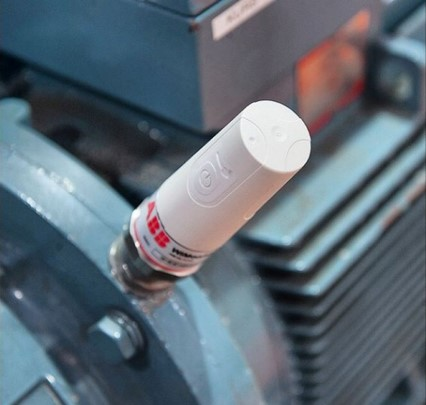
\includegraphics[width=0.6\textwidth]{INTRO/Figs/StateOfArt/abb.jpg}
        \end{figure} 
        
    \subsection{IFM VSExxx}
        IFM je německá firma se zaměřením na senzoriku v průmyslu. Přidaná hodnota produktů této společnosti tkví zejména v široké nabídce nabízených řešení. Koncový zákazník si může podle svých požadavků sestavit celý monitorovací systém. IFM nabízí různě kvalitní akcelerometry, vzorkovací obvody a monitorovací jednotky \cite{manufactor:2}. Na rozdíl od firmy ABB lze prostřednictvím dodaného softwaru VES004 konfigurovat parametry monitorování, a docílit tak různorodějších analýz. Systém nevyužívá brány, k jednotlivým jednotkám lze ale připojit více akcelerometrů. Zásadní odlišností od ostatních porovnávaných systémů je drátová komunikační infrastruktura, jejíž nasazení se příliš nehodí do již fungujících průmyslových prostředí (více v kapitole \ref{section:drat}).
        
         \begin{itemize}
            \item Konektivita: Ethernet
            \item Konfigurovatelnost: nastavitelné jsou standardní parametry monitorování
            \item Software: desktopová aplikace bez propojení s cloudem
            \item Přesnost: rozdílná podle konkrétního řešení
            \item Napájení: síťové 
            \item Cena: rozdílná podle konkrétního řešení
        \end{itemize}{}
        
        \begin{figure}[!htp]
            \centering
            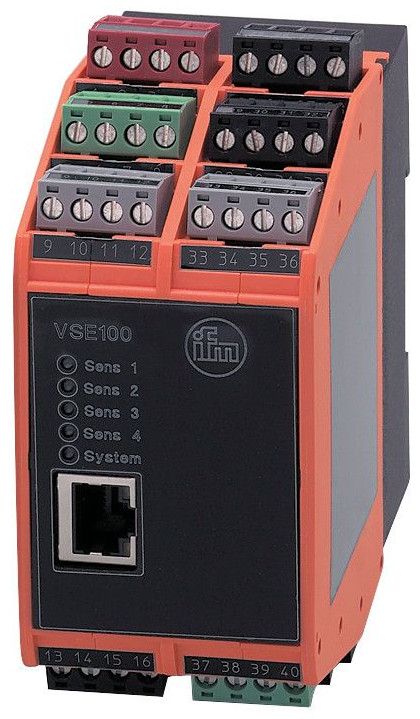
\includegraphics[width=0.25\textwidth]{INTRO/Figs/StateOfArt/ifm2.jpg}
            \caption {Jednotka VSE002 pro připojení 4 akcelerometrů. Převzato z \cite{manufactor:2}.}
        \end{figure}
        
       
        
       
       \begin{figure}[!htp]
            \centering
            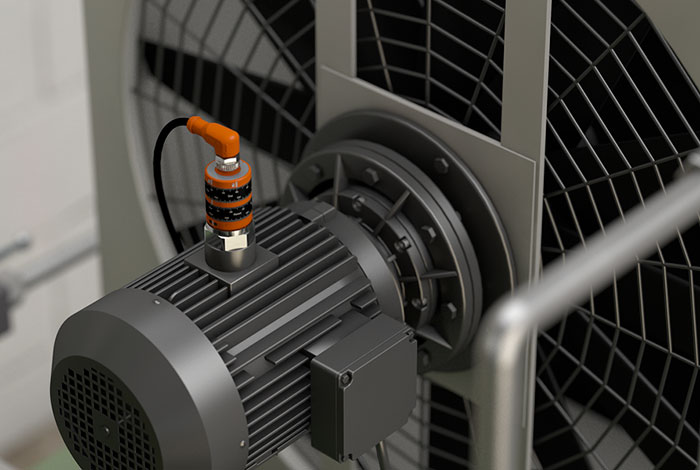
\includegraphics[width=0.7\textwidth]{INTRO/Figs/StateOfArt/ifm3.jpg}
            \caption {Upevnění akcelerometru VSE002 k motoru. Převzato z \cite{manufactor:2}.}
        \end{figure}
    
    
    \subsection{Fluke 3561 FC Vibration Sensors}
        Fluke je americká společnost zaměřující se na elektronické monitorovací a testovací systémy. Jejich produkty si na rozdíl od ABB a IFM zakládají na inovaci, a proto Fluke přináší z hlediska filosofie IIoT mnohem modernější monitorovací systém, kde vlastní diagnostika probíhá za pomocí webového klienta a mobilní aplikace. Za zmínku stojí také velmi elegantně vyřešený design, velikost a možnosti upevnění senzorů k motorům \cite{manufactor:3}.
        
     
        
        \begin{itemize}
            \item Konektivita: Low power Bluetooth 
            \item Konfigurovatelnost: pevná vzorkovací frekvence, odesílání informací do brány
            \item Software: zpracování dat prostřednictvím Fluke Connect App
            \item Přesnost: $\pm 32\,g$, šířka pásma 1 kHz
            \item Napájení: bateriové zařízení s výdrží 5 let
            \item Cena: zhruba 100 000 Kč za 4 senzory, 1 bránu a software
        \end{itemize}{}
        
          \begin{figure} [!htp]
            \centering
            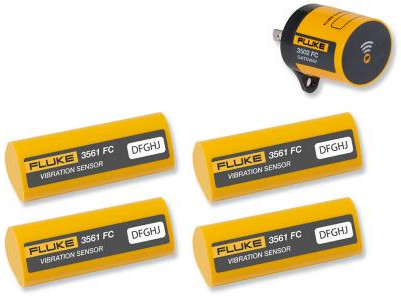
\includegraphics[width=0.4\textwidth]{INTRO/Figs/StateOfArt/fluke2.jpg}
            \caption {Brána a monitorovací jednotky Fluke. Převzato z \cite{manufactor:3}.}
        \end{figure}
    
        
        \begin{figure}[H]
            \centering
            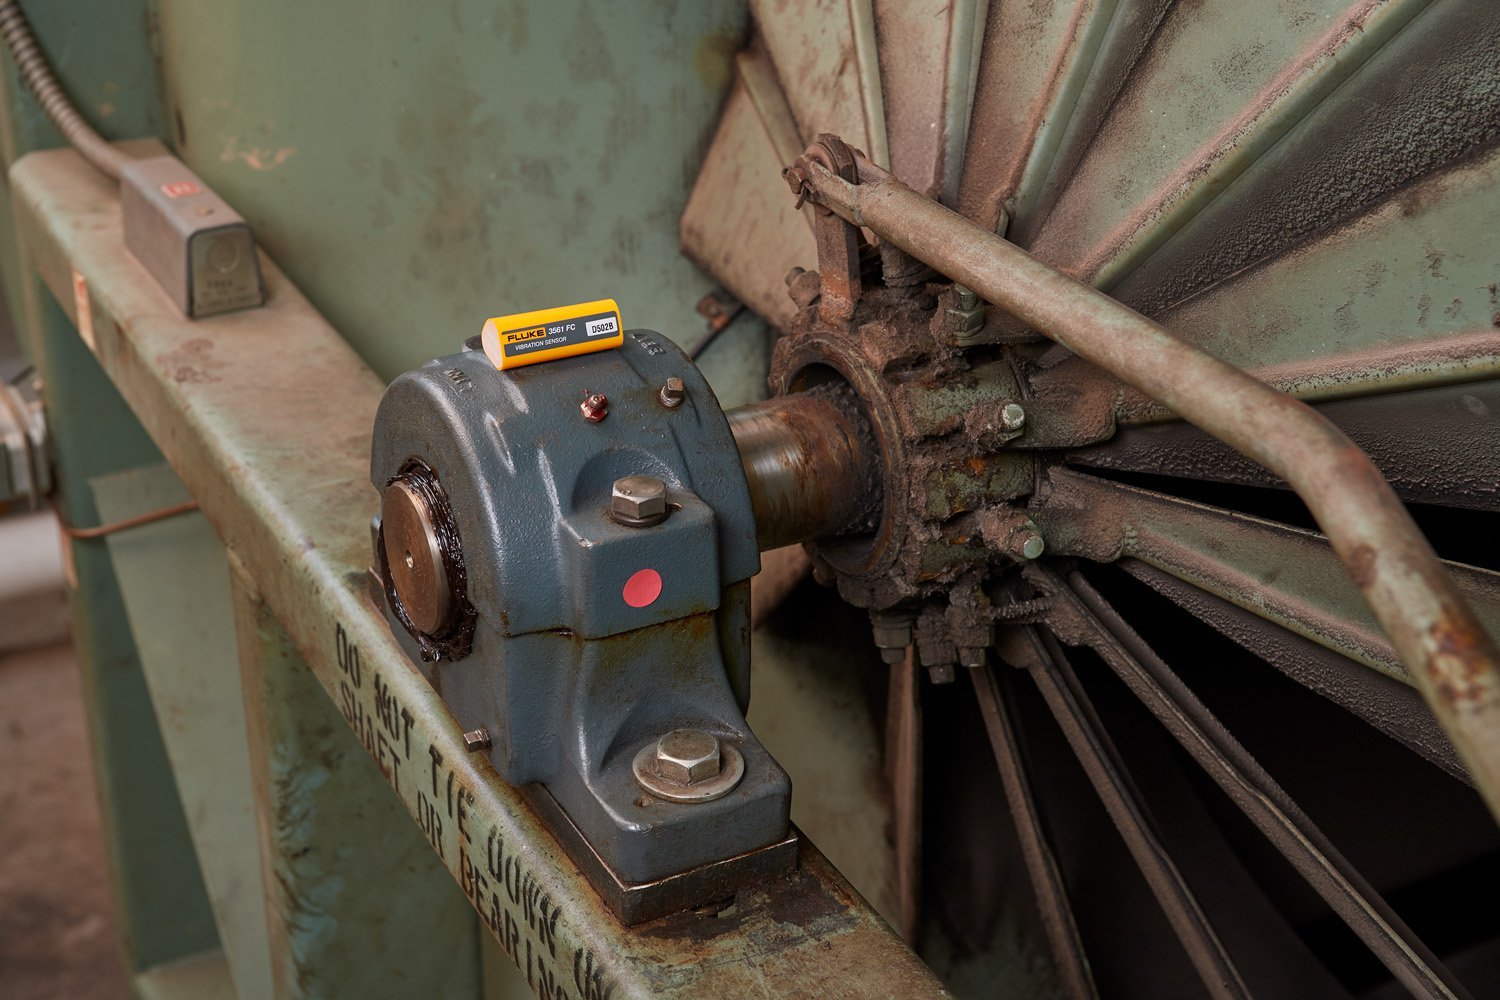
\includegraphics[width=0.75\textwidth]{INTRO/Figs/StateOfArt/fluke.jpg}
            \caption {Upevnění Fluke senzoru k motoru. Převzato z \cite{manufactor:3}.}
        \end{figure}

    
    
    \subsection{Flexs C2 Wireless Condition Analyzer}
        Společnost FlexSCADA je kanadská společnost zabývající se SCADA (Supervisory Control And Data Acquisition) systémy, tedy sběrem dat a řízením. Produkty této společnosti jsou nejflexibilnějšími, které se mi podařilo nalézt. Umožňuje především široké možnosti konfigurace monitorování (nastavení vzorkovací frekvence, počet vzorků u FFT, interval odesílání dat\ldots). Navíc přichází se zajímavým řešením, kdy po stisknutí tlačítka vytvoří zařízení hotspot, ke kterému se lze přihlásit a pozorovat současné trendy monitorování. Krom toho ale odesílá data i do cloudu ke specifičtějším analýzám \cite{manufactor:4}.\\
        Problémem jsou pouze vysoké pořizovací náklady v případě nasazení systému do velkých továren. Ačkoliv cena jednoho monitorovacího zařízení je poměrně přívětivá a najednou lze díky čtyřem akcelerometrům připojit více motorů, s~narůstajícím počtem monitorovaných zařízení cena rychle roste.
        \begin{itemize}
            \item Konektivita: WiFi, LTE
            \item Konfigurovatelnost: široká možnost konfigurace včetně parametrů monitorování
            \item Software: webový klient a aplikace + možnost odesílání dat a zpracování v cloudu
            \item Přesnost: nespecifikováno
            \item Napájení: sběr energie z elektromagnetického vyzařování, externí síťové napájení
            \item Cena: zhruba 25 000 Kč za jednotku pro maximálně čtyři motory.
        \end{itemize}{}
        
        \begin{figure} [!h]
                \centering
                \caption{FlexSCADA Condition Analyzer. Převzato z \cite{manufactor:4}.}
                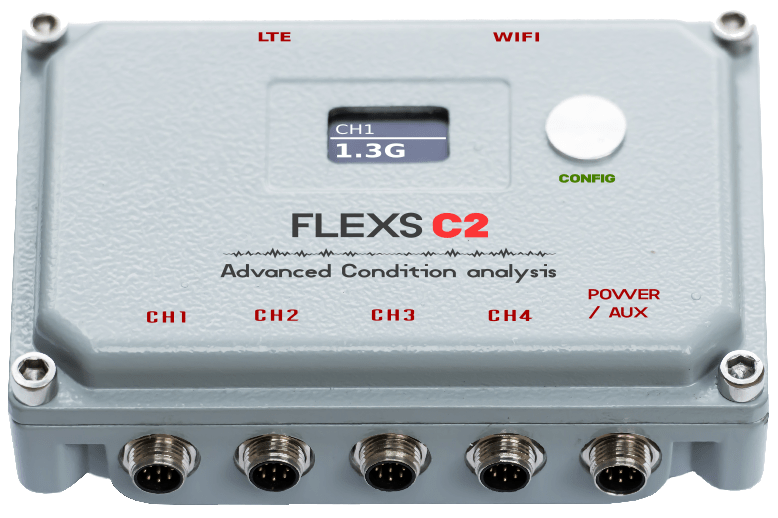
\includegraphics[width=0.7\textwidth]{INTRO/Figs/StateOfArt/flexscada.png}
        \end{figure} 


\section{Cíl práce}
    
    Cílem této práce bylo navrhnout a realizovat komplexní systém pro monitorování stavu rotačních zařízení pomocí pokročilé analýzy vibrací a teploty. Snahou bylo odlišit se od existujících řešení, vyplnit mezeru na trhu a postavit systém na základech moderních konceptů IIoT.\\
    
    \textbf{Konfigurovatelnost}
    
    Sytém se bude odlišovat od existujících zařízení na trhu zejména svoji konfigurovatelností. Uživatel bude moci pohodlně ve webovém prostředí měnit parametry monitorovací jednotky, díky čemuž bude schopen přizpůsobit zpracování monitorovaných veličin, a dosáhnout tak různorodějších a pokročilejších analýz.\\
    
    \textbf{Bezdrátová komunikace na velké vzdálenosti}
    
    Důraz bude kladen na dostupnost a univerzální použití za pomoci LPWAN sítí. Jako komunikační síť se bude využívat LoRa s velkým dosahem, nízkým datovým tokem a vysokou výdrží baterie, což umožní monitorovat stav rotačních zařízení i v případech, kdy to dříve nebylo možné (více v kapitole \ref{section:lpwan}).
    
    \textbf{Nezávislost}
    
    Systém bude také zcela nezávislý na již existujících oficiálních LoRa sítích jako The Things Network či síti Českých Radiokomunikací. Krom koncových uzlů bude tedy zahrnovat i centrální jednotku (Gateway) pro řízení komunikace s měřicími jednotkami a komunikaci s~aplikačním serverem. Tento přístup usnadňuje nasazení systému i do míst, která nejsou pokrytá signálem, nebo mají problémy s jeho silou.
    
    \textbf{Flexibilita a otevřenost}
    
   Pozornost bude věnována flexibilitě celého systému prostřednictvím použití databázového modelu a RESTového serveru, které umožní poskytnutí naměřených a vypočítaných dat aplikacím třetích stran. Díky této otevřenosti systému budou zákazníci moci data zpracovávat podle svých požadavků a snadněji je integrovat do vlastních systémů.
   
   \textbf{Cena}
   
   Vzhledem k tomu, že produkt je studentskou prací, cena celého systému bude tlačena co možná nejníže.
   
%CHECK ~
%CHECK red
%CHECK ...
% %!TEX ROOT=ctutest.tex
\chapter{Využití LPWAN sítí v IIoT}
    Současným trendem v~průmyslu je vysoký nárůst počtu připojených zařízení – v~ roce 2019 se očekává navýšení o 10 \% \cite{website:1}. S tímto faktorem je spojena především snaha o chytřejší monitorování výrobních procesů a sběr dat. Z~analýzy firmy HMS Network lze proto jasně vidět, že dnešní tendencí v~průmyslu je přechod na komunikační technologie umožňující snadné propojení průmyslových systémů s IIoT aplikacemi jako jsou EtherNet/IP a bezdrátové technologie jako WiFi, Bluetooth nebo LPWAN \cite{website:1}.\\
    Připojení velkého množství senzorů do již existujících průmyslových hal představuje jeden z hlavních problémů, se kterým se musejí nové komunikační sítě vypořádat.
    
   
\section{Drátové vs bezdrátové sítě v~průmyslu}
\label{section:drat}
    V~posledním roce zaznamenaly bezdrátové sítě nejvyšší nárůst (o 30 \%)  ze všech průmyslových komunikačních technologií \cite{website:1}, avšak zastoupení drátových technologií jako je Industrial Ethernet (EtherNet/IP, Ethernet Powerlink, EtherCat, PROFINET) nebo Fieldbus stále představuje většinový podíl na trhu.
    
    \begin{figure} [!ht]
        \centering
        \caption{Rozdělení komunikačních technologií v~průmyslu v~roce 2019. Převzato z \cite{website:1}.}
        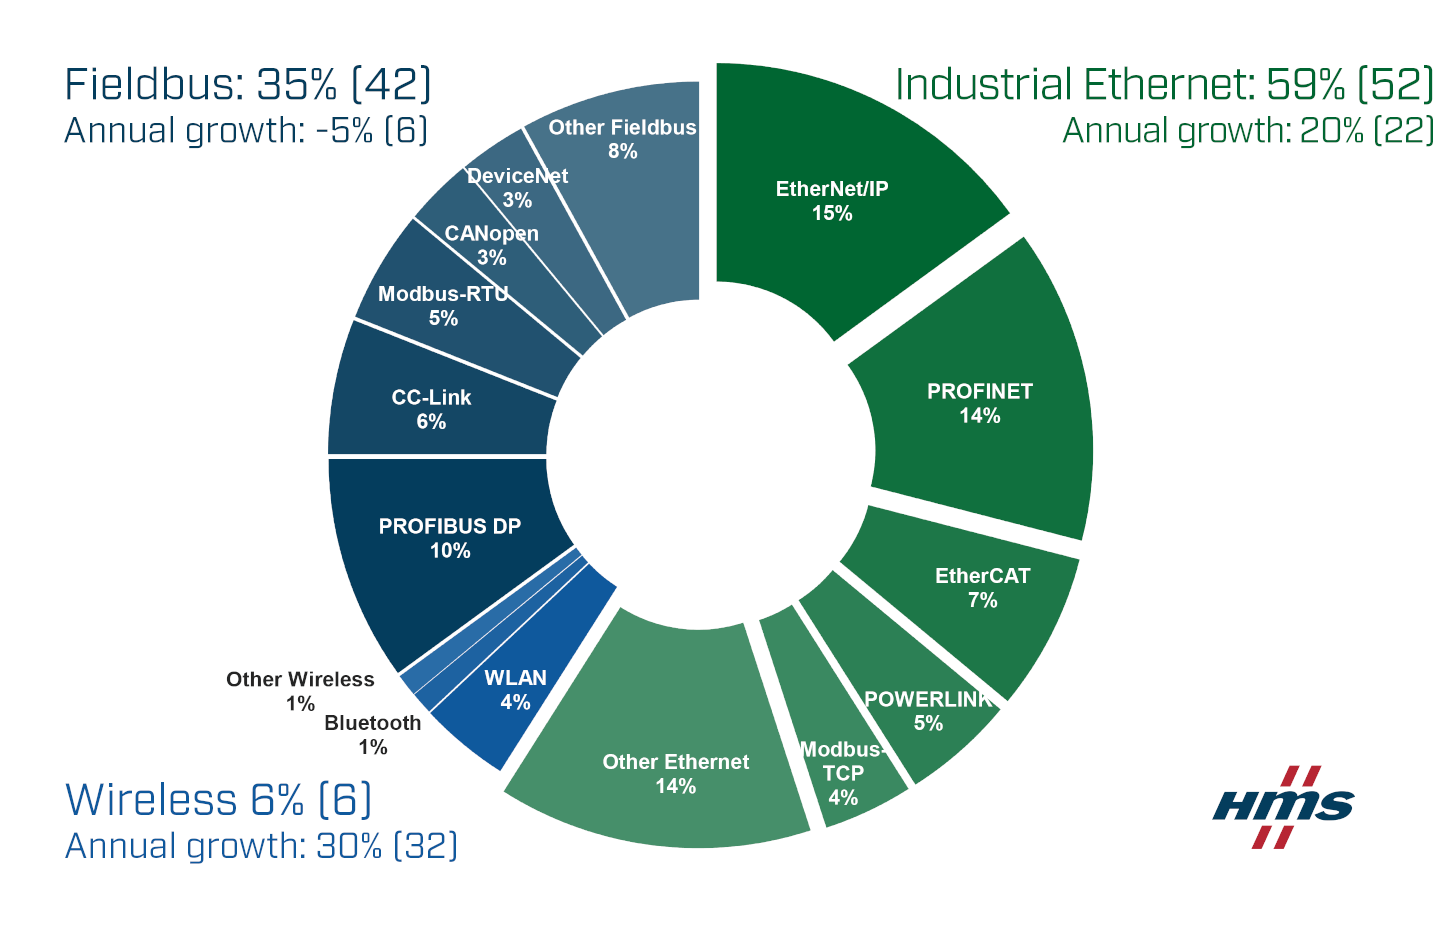
\includegraphics[width=\textwidth]{LPWAN/Figs/networkshares2019.png}
    \end{figure} 
    
    Nasazení bezdrátových technologií ovšem nemá za cíl zcela nahradit komunikaci drátovou. Pro průmyslovou automatizaci, řídící aplikace a real-timové procesy s vysokými nároky na spolehlivost jako je řízení výrobních linek, budou i nadále upřednostňovány spolehlivé a roky odzkoušené protokoly jako PROFINET či ProfiBus.\\
    Pro monitorovací aplikace v~rámci CBM, jež vyžadují připojení velkého množství senzorů, jsou ale tyto technologie příliš těžkopádné a drahé. Hlavní problém také představuje fakt, že v~mnoha případech není možné zasahovat do již fungují komunikační infrastruktury, odstavovat výrobu, a proto převládá snaha novými senzory pouze doplnit stávající řešení \cite{website:3}.\\
    Jsou to tedy především jednoduchost instalace, dosah a spotřeba, proč se v~posledních letech mohutně využívají ve výrobních prostředích bezdrátové sítě. 

\section{LPWAN mezi bezdrátovými IIoT sítěmi}
\label{section:lpwan}
    LPWAN (Low Power Wide Area Network) je rodina bezdrátových sítí určená pro vysoký dosah, nízký datový tok a nízkou energetickou spotřebu, a zejména tak vhodná pro bateriová zařízení. LPWAN technologie také využívají k~připojení zařízení menší šířku frekvenčního pásma, než je obvyklé u~běžně využívaných zařízení u mobilních sítí \cite{website:3}.\\
    Hlavními a prvotními zástupci LPWAN sítí jsou LoRa a SigFox, které jsou provozovány v~bezlicenčních ISM pásmech na kmitočtech 863-870 MHz v~Evropě a 902-928 MHz v~USA \cite{website:5}.\\
    Dále síť NB-IoT fungující v~licencovaných pásmech vlastněných mobilními operátory, kterou proto lze provozovat na již existující mobilní komunikační infrastruktuře pouhou softwarovou úpravou, kdy se vysílacím stanicím vyhradí speciální část pásma. Na rozdíl od sítí Sigfox a LoRa tedy není nutné instalovat žádné dodatečné vysílače \cite{website:4}.
    
    
    LPWAN sítě řeší mnoho problémů, se kterými se potýkají sítě krátkého dosahu (WiFi, Bluetooth\ldots) a celulární mobilní sítě (GSM, GPRS, LTE\ldots). Umožňují bezdrátové připojení senzorů a monitorování i na rozlehlých plochách s velkými vzdálenostmi (stavební plochy, větrné elektrárny) nebo obtížně dostupných místech (malé vodní elektrárny \cite{website:2}, kryty, tunely), kde nasazení monitorovacích systémů nebylo dříve možné nebo bylo velmi finančně nákladné.
    
    
    Ve srovnání s WiFi a Bluetooth je jejich hlavní výhodou především zmíněný vyšší dosah, propustnost ve vnitřních prostorách (tzv. building penetration). U~sítě LoRa pak také díky komunikaci v~rozprostřeném spektru odolnost vůči úzkopásmovému elektromagnetickému rušení, které představuje problém nejen díky přeplnění WiFi kanálů, ale také kvůli průmyslovým strojům jako jsou vysokozdvižné vozíky, jež by často ani neprošly kontrolami EMC.\\
    Hlavním benefitem na rozdíl od mobilních sítí je zejména výdrž baterie. Často se také může stát, že rádiový signál je částečně odstíněn krytem výrobní haly, což lze u LPWAN sítí snadněji vyřešit nasazením brány do vnitřku budovy než u mobilních sítí.

    
\section{Komunikační řetězec LPWAN sítě}
    \begin{figure} [!ht]
        \centering
        \caption{Komunikační řetězec LPWAN sítí. Převzato z \cite{website:4}.}
        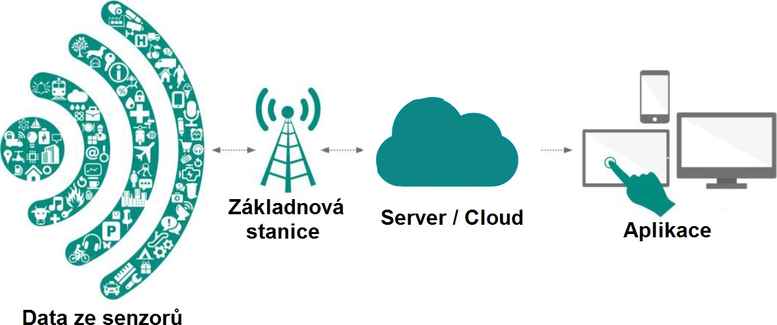
\includegraphics[width=\textwidth]{LPWAN/Figs/communication_chain.png}
    \end{figure} 
    LPWAN síť je tvořená z koncových uzlů využívajících určitý komunikační protokol a odesílajících data do základových stanic (bran), jež data dále přeposílají na vzdálený server, na který jsou napojené aplikace koncových zákazníků.\\
    Uvedené příklady LPWAN sítí (LoRa, Sigfox, NB-IoT) využívají hvězdicovitou topologii \cite{website:4}, kde jednotlivé uzly komunikují vždy pouze s branami, což usnadňuje řízení chodu sítě (není třeba používat složité směrovací protokoly) a usnadňuje její rozšiřování. Středem sítě je poté řídící server, který zajišťuje směrování paketů danému adresátovi.
    
\section{$\text{LoRa}^{\text{TM}}$}
    LoRa, představující zkratku pro slova Long Range, je jeden z hlavních zástupců LPWAN sítí a současně označení pro fyzickou (PHY) vrstvu této proprietární technologie vlastněné francouzskou firmou Semtech. Linková (MAC) vrstva poté nese označení LoRaWAN .\\
    Fyzická vrstva sítě LoRa využívá modulaci s rozprostřeným spektrem, konkrétně variantu modulace CSS (Chirp Spread Spectrum), kdy je přenášená informace modulována na nosný signál, který je lineárně rozmítán od vrchní hranice pásma (bandwidth) po jeho spodní hranici. Strmost tohoto rozmítání určuje parametr označovaný jako Sperading Factor (česky činitel rozprostření, dále pouze jako SF), který tak ovlivňuje rychlost komunikace \cite{manual:1}.\\
    
    \begin{figure} [!ht]
        \centering
        \caption{LoRa modulace – porovnání strmosti rozmítání SF 7-12. Převzato z \cite{picture_website:1}.}
        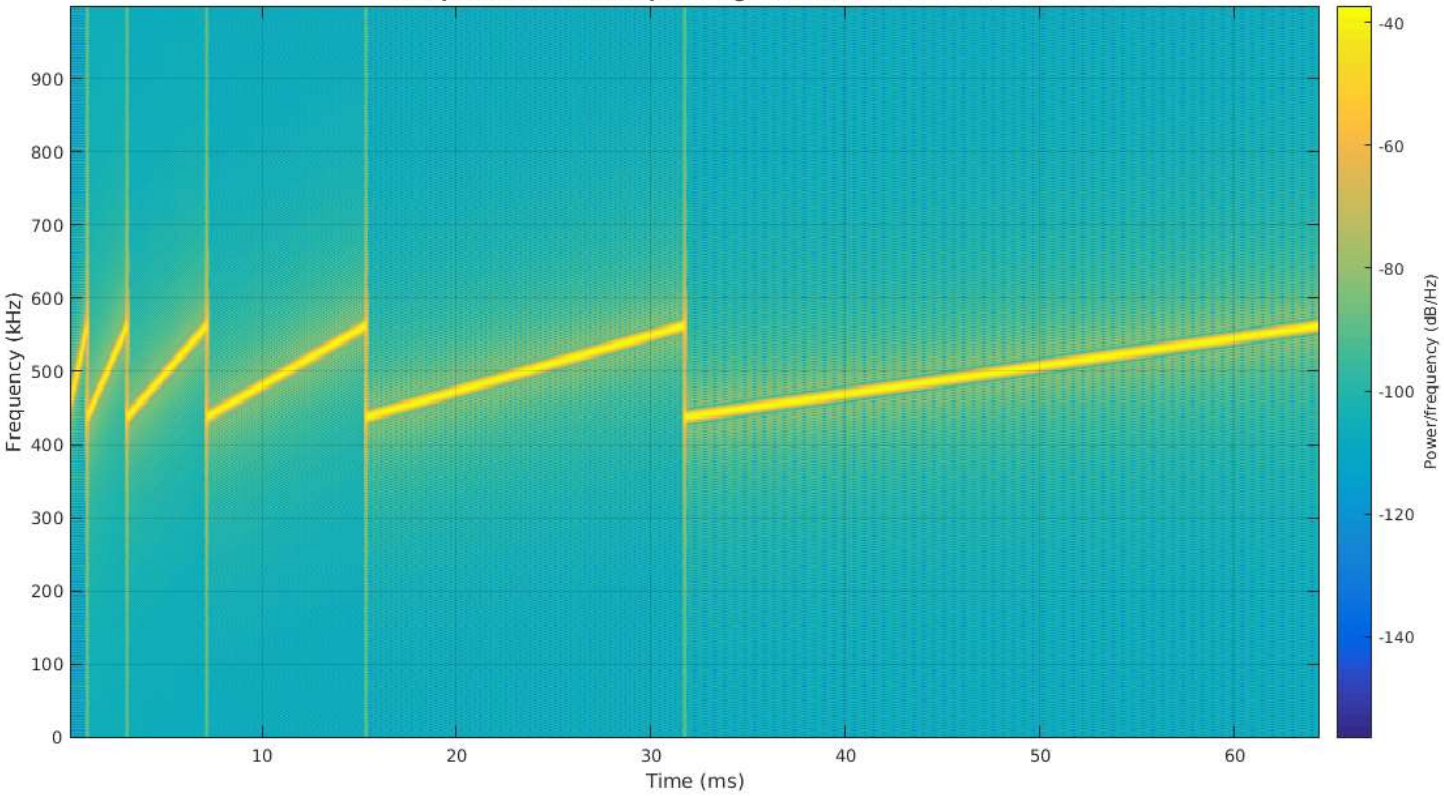
\includegraphics[width=0.9\textwidth]{LPWAN/Figs/lora_sf.png}
    \end{figure} 
    
    Komunikace v~rozprostřeném spektru byla původně vytvořena kvůli vojenským účelům pro minimalizaci možnosti odposlechu, ale dnes se tato technika využívá zejména díky odolnosti vůči úzkopásmovému rušení. Další výhodou jsou samoopravné kódy FEC (Forward Error Correction), větší dosah (ve volném prostranství kolem 10 km) s možností přijímat vysílaný signál až 20 dB pod úrovní šumu, odolnost vůči Doplerovu jevu a potřeba menšího vysílacího výkonu redukujícího spotřebu energie \cite{manual:1}.
    
    \begin{figure} [!ht]
        \centering
        \caption{Komunikace pod úrovní hladiny šumu. Převzato z \cite{picture_website:2}.}
        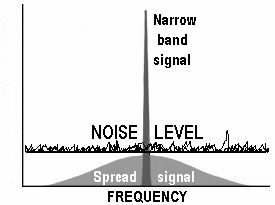
\includegraphics[width=0.6\textwidth]{LPWAN/Figs/lora_noise.jpg}
    \end{figure} 
    

\section{LoRa jako použítá LPWAN síť}
\label{section:single_channel_gw}
    I přes značné výhody NB-IoT v~podobě přenosové rychlosti a pokrytí byla nakonec pro účely této práce  jako komunikační médium zvolena síť LoRa a to především díky ceně rádiových čipů, které jsou kvůli využití bezlicenčních pásem řádově menší.
    
    Mezi cíle práce patří také vytvořit soběstačný systém komunikující oběma směry, nezávislý na pokrytí oficiálních LoRa bran, a proto bylo nutné vytvořit i vlastní bránu.\\
    Kvůli cenovým důvodům navržená brána využívá LoRa čip určený pro koncová zařízení, jehož nevýhoda oproti čipům pro oficiální brány spočívá v~možnosti komunikovat v~danou chvíli pouze na jednom kanálu, a jedná se tak pouze o~tzv. jednokanálovou bránu – anglicky Single channel gateway (více v~kapitole \ref{section:semtech_chips}). Využívaný komunikační kanál a spreading factor tedy musí být u uzlu a jednokanálové brány pro úspěšnou komunikaci předem určen, a nemá smysl proto implementovat LoRaWAN protokol.
    
      \begin{figure} [!ht]
        \centering
        \caption{Oficiální LoRa brána od firmy Multitech využívající čipy SX13xx. Převzato z \cite{website:10}.}
        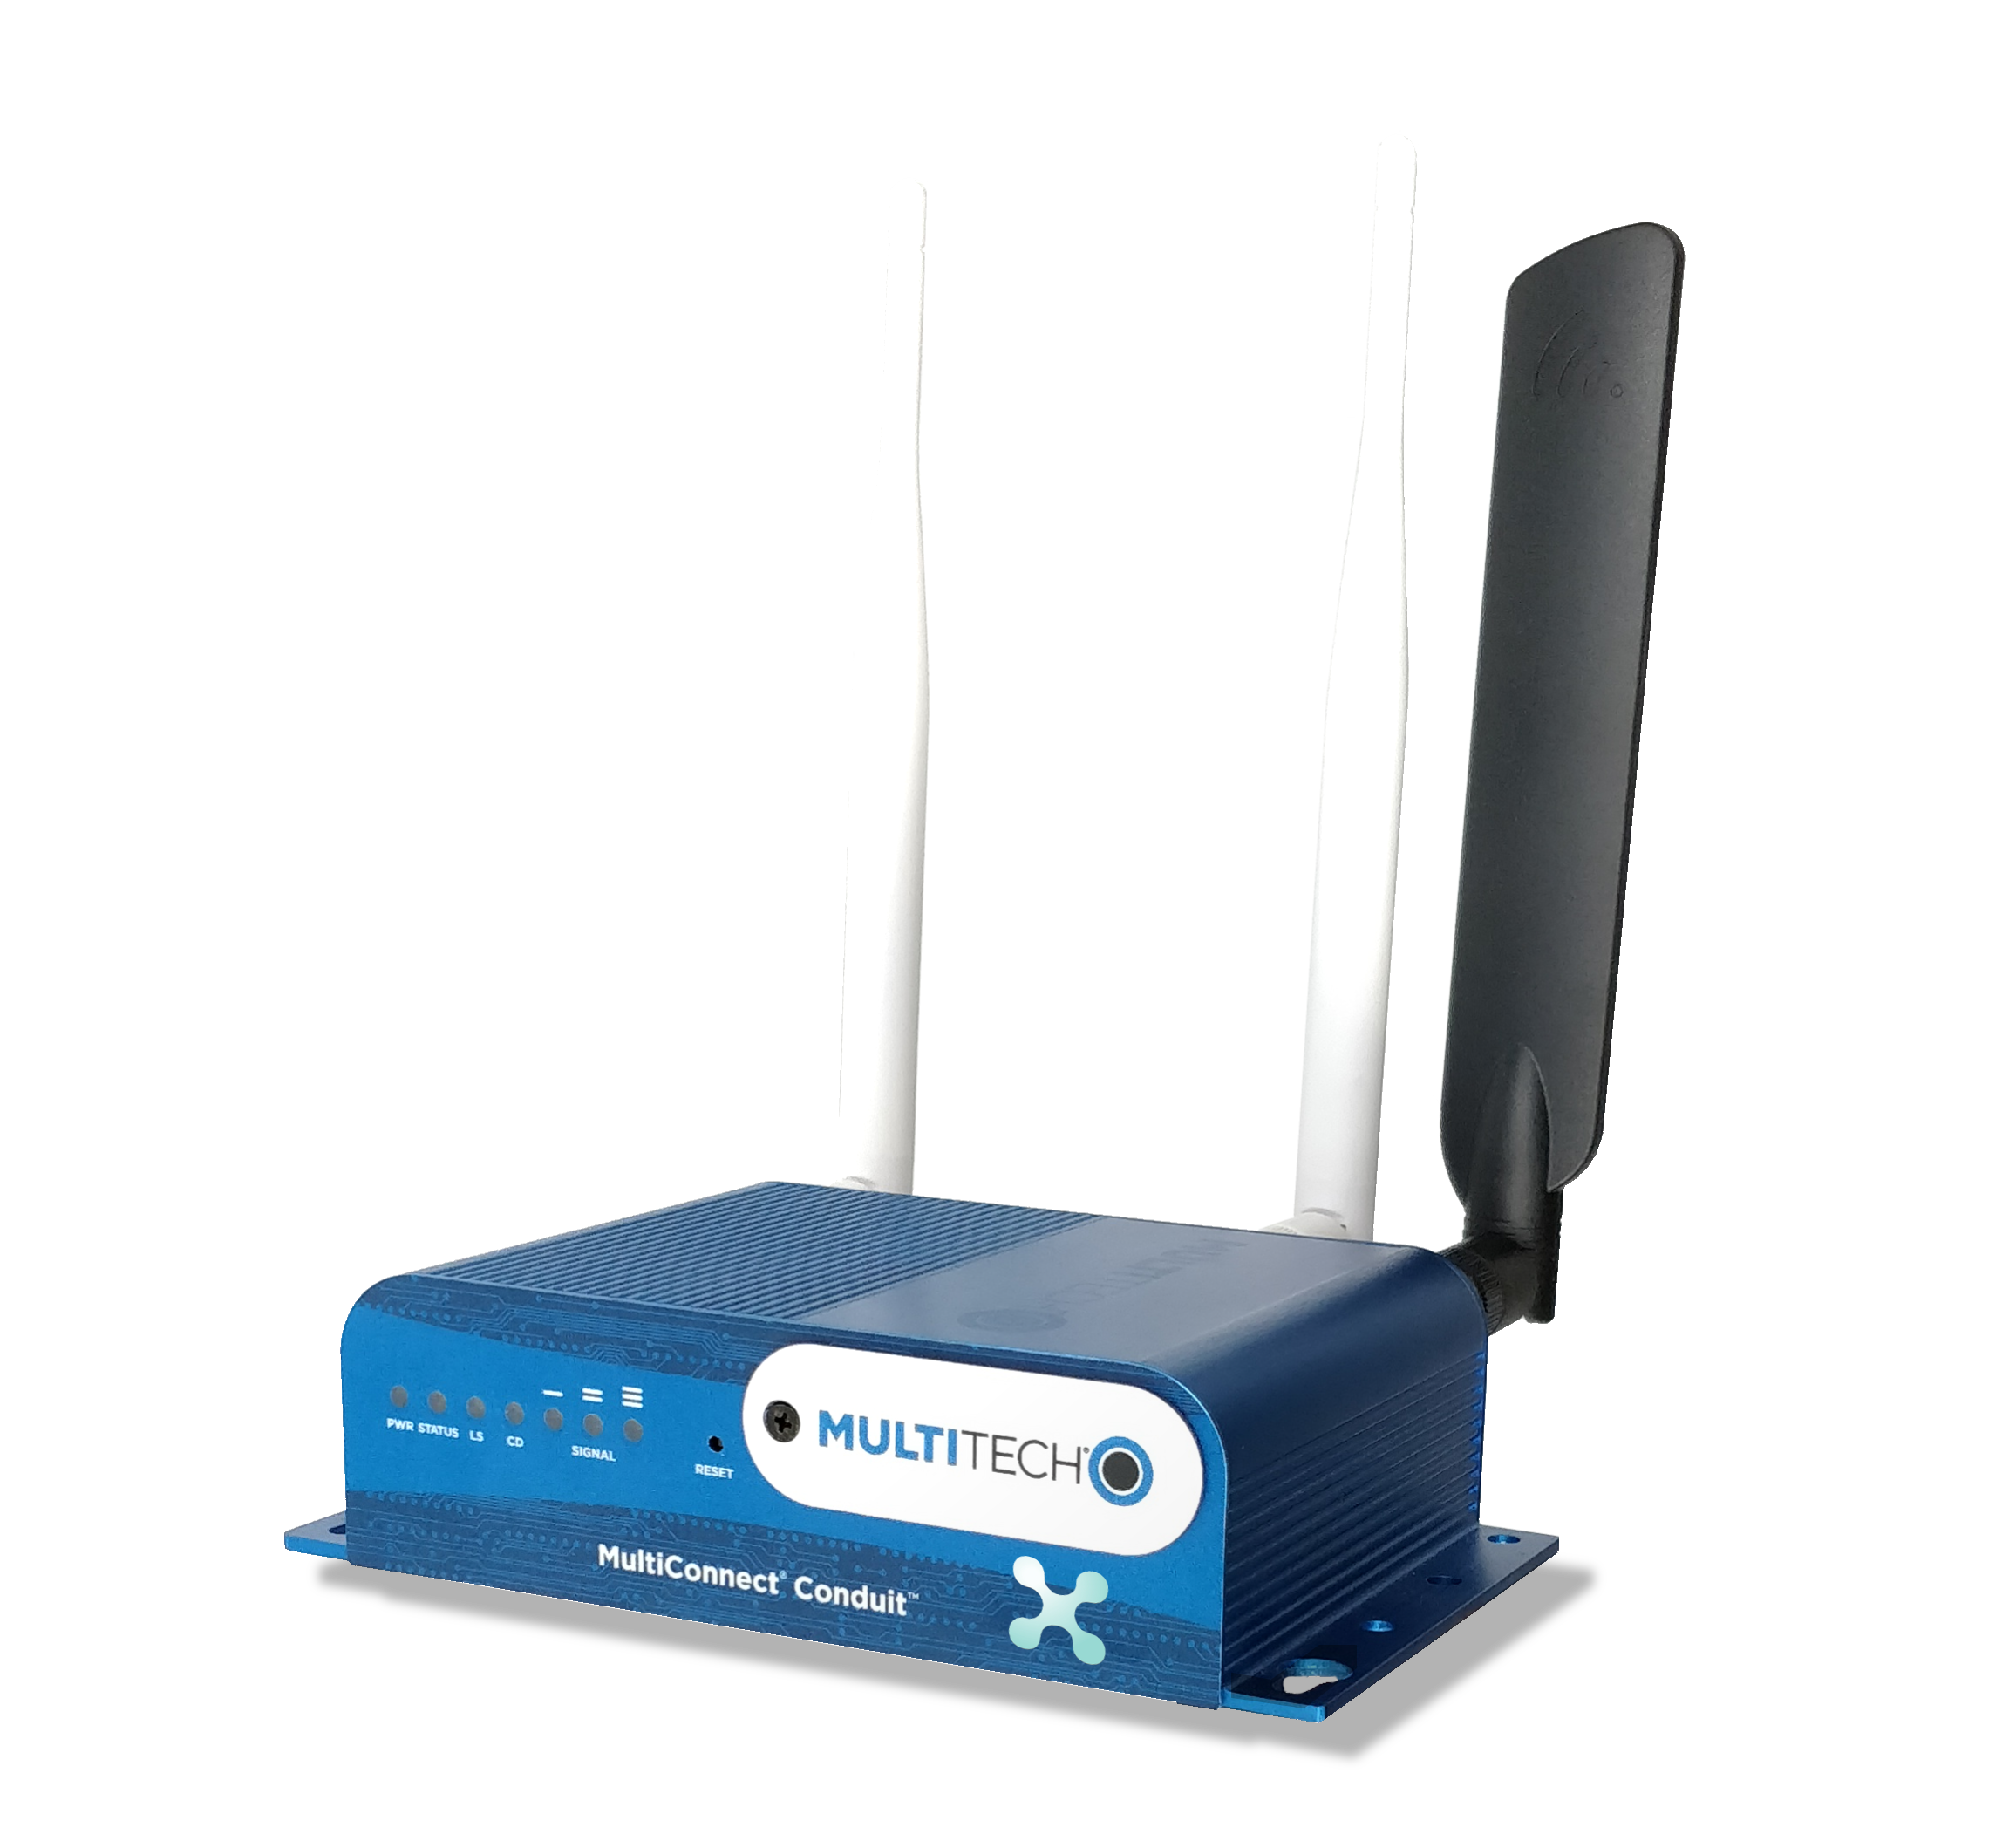
\includegraphics[width=0.8\textwidth]{LPWAN/Figs/lorawan_gw.png}
    \end{figure} 
    
%CHECK ~
%CHECK red
%CHECK ...



% ZDROJE
% https://www.designworldonline.com/industrial-ethernet-takes-the-lead-over-fieldbuses-says-study/

% https://www.automation.com/automation-news/article/lpwan-as-the-new-sensor-communication-infrastructure-for-iiot

% https://www.thethingsnetwork.org/docs/lorawan/frequency-plans.html

% https://elektro.tzb-info.cz/informacni-a-telekomunikacni-technologie/16519-site-pro-internet-veci-v-ceske-republice

% [5]
% https://www.link-labs.com/blog/iot-topology

% [6]
% Rashmi Sharan Sinha, Yiqiao Wei, and Seung-Hoon Hwang. A survey on
% LPWAN technology: LoRa and NB-IoT. ICT Express, 3(1):14–21, 3 2017

% [7] https://www.semtech.com/uploads/documents/an1200.22.pdf
% LPWAN obrazek
% https://medium.com/coinmonks/lpwan-lora-lorawan-and-the-internet-of-things-aed7d5975d5d

% LoRa chirp
% https://fenix.tecnico.ulisboa.pt/downloadFile/1689468335603030/LoRaWAN\%20Introduction.pdf


% https://www.semtech.com/

% Noise 
% https://www.instructables.com/id/Introducing-LoRa-/
% %!TEX ROOT=ctutest.tex
\chapter{Vibrační signály a jejich digitální zpracování}

    Vibrační analýza je samotnou podstatou celé práce. Tato kapitola se snaží vysvětlit původ vibračního signálu a techniky jeho zpracování.

\section{Poruchy indukčních motorů}
\label{section:poruchy_mororu}
    K selhání motorů může dojít mnoha způsoby. Může se jednat o poškození vinutí statoru, defekt rotoru, ale statistika ukazuje, že 40 až 90 \% poruch je zapříčiněno defektem ložisek \cite{book:1}, jejichž původ může být různého druhu, jak ukazuje následující seznam \cite{prez:1}.
    \begin{figure} [!h]
        \centering
        \caption{Příčiny poruch indukčních motorů. Převzato z \cite{prez:2}.}
        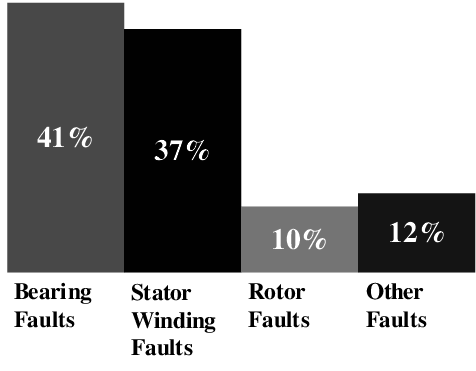
\includegraphics[width=0.4\textwidth]{DSP/Figs/failures.png}
    \end{figure} 
   
    \begin{itemize}
        \item Vady před uvedením do provozu – rozměrové a tvarové nepřesnosti, brusné trhliny.
        \item Vady způsobené nesprávným upevněním k hřídeli – nesouosost, excentricita.
        \item Vady způsobené únavou materiálu ve valivém styku – povrchová styková únava.
        \item Vady způsobené vnějšími vlivy – mazání, znečištění, koroze.
    \end{itemize}
    
    \begin{figure} [!h]
        \centering
        \caption{Příklady poškození ložisek}
        \begin{subfigure}[b]{0.48\textwidth}
             \centering
             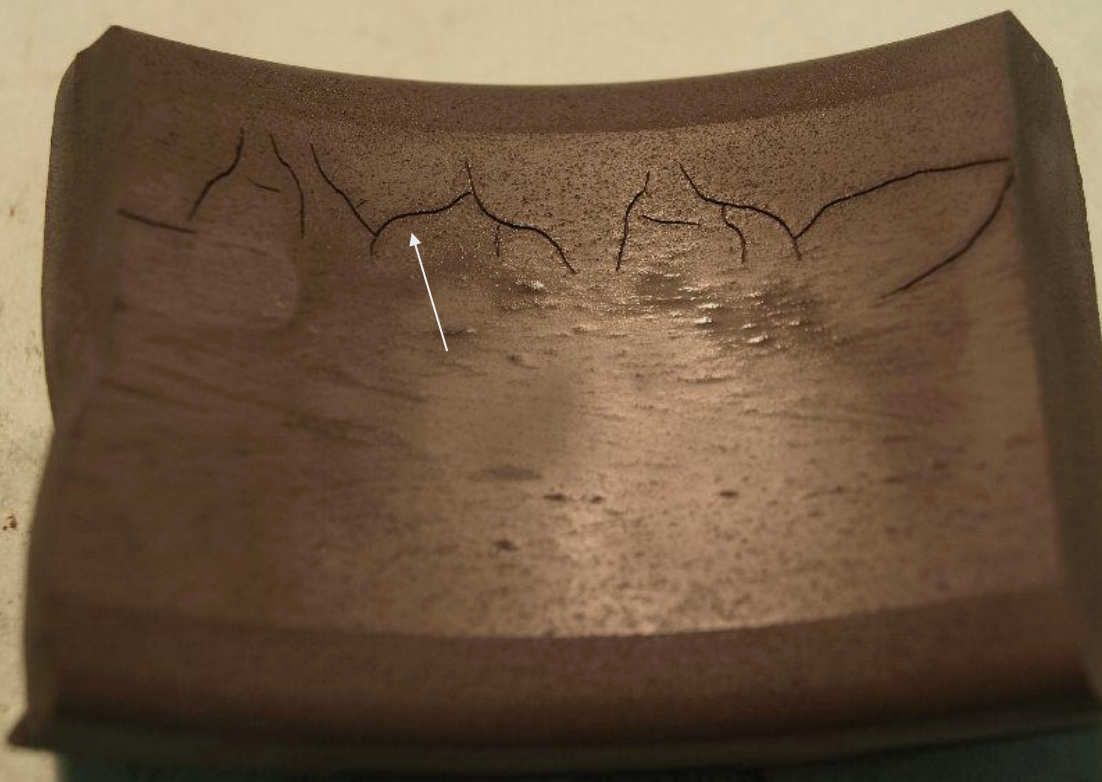
\includegraphics[width=\textwidth]{DSP/Figs/poruchy_lozisek.png}
             \caption {Brusné trhliny na vnitřním kroužku. Převzato z \cite{prez:1}.}
         \end{subfigure}
         \hfill
        \begin{subfigure}[b]{0.46\textwidth}
            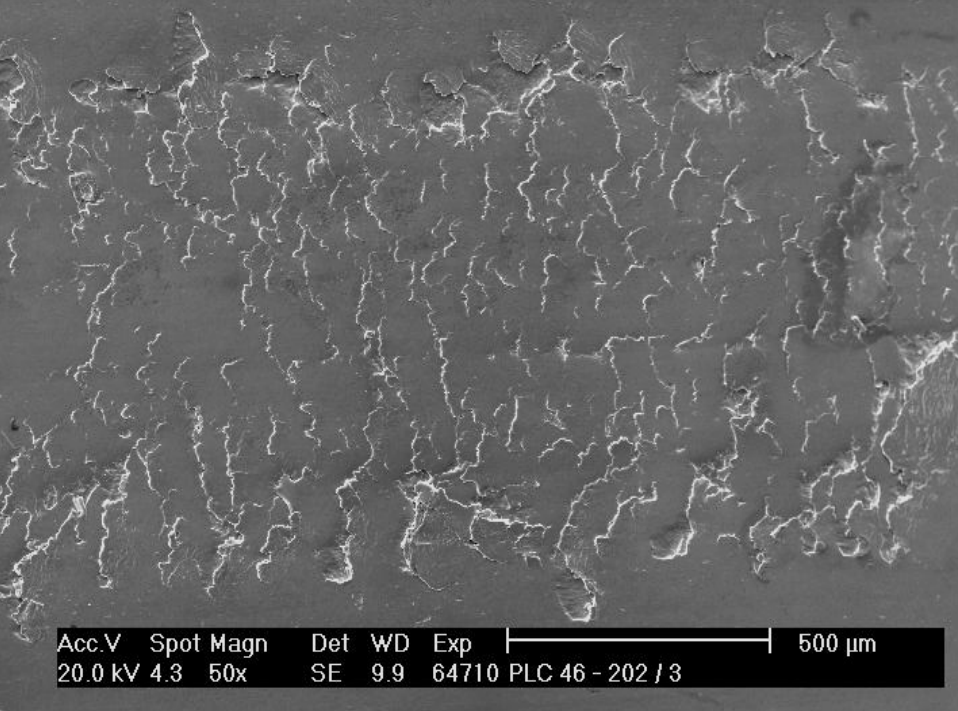
\includegraphics[width=\textwidth]{DSP/Figs/poruchy_lozisek2.png}
            \caption {Povrchové únavové poškození, tzv. pitting. Převzato z \cite{prez:1}.}
        \end{subfigure}
    \end{figure} 
    
    
    
    Analýza vibrací je nejpoužívanější a nejpřínosnější metodou diagnostiky poruch rotačních zařízení \cite{book:1}. Pomocí vibrací lze diagnostikovat poruchu už v~jejím raném stádiu – až měsíce před tím, než dojde k úplnému selhání stroje, což je mnohem dříve než je tomu u ostatních veličin, které lze monitorovat, jako akustických emisí, tepla nebo proudového odběru (viz obrázek \ref{figure:condition}).\\
    Všechna rotační zařízení bez ohledu na dobu provozu a opotřebení vytvářejí vibrace. 
    Vibrační signál motoru v sobě tedy nese velké množství informací, jejichž povaha se navíc po dobu provozu postupně mění. Vlastnosti tohoto signálu jsou determinovány jednotlivými částmi motoru (hřídel, převodovka, turbína, ložiska\ldots) a také v sobě reflektují jeho vady a nedokonalosti.
    Správné porozumění a interpretace těchto vlastností spojená s vhodnými analýzami a technikami zpracování signálu je tedy klíčová pro určení vznikajících poruch při CBM.
    
    \begin{figure} [!h]
        \centering
        \caption{Výhody analýzy vibrací. Převzato z \cite{prez:2}.}
        \label{figure:condition}
        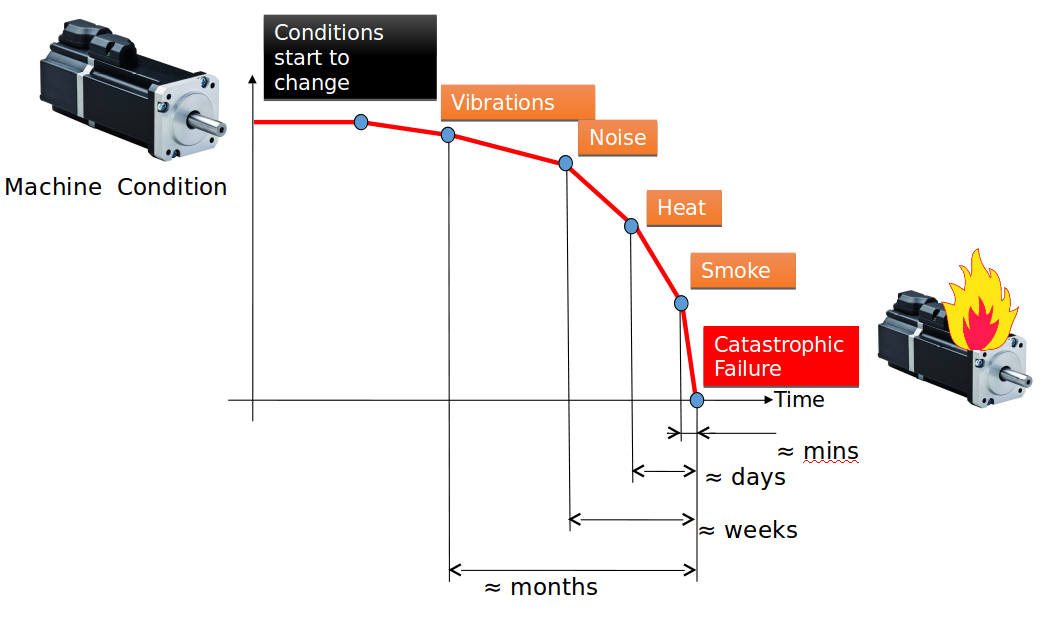
\includegraphics[width=0.8\textwidth]{DSP/Figs/condition.png}
    \end{figure} 

\section{Snímání vibračního signálu}
\label{section:measuring}
    Vibrační signál se získává prostřednictvím měření akcelerace na určitém místě motoru. Kvalita naměřeného signálu silně závisí na umístění akcelerometru v~rámci zařízení. Vibrace lze měřit ve směru osy motoru a ve dvou zbývajících osách kolmých na osu motoru, které bývají pro monitorování důležitější. Můžeme tedy použít jeden trojosý akcelerometr, nebo tři jednoosé. Frekvence signálu se obvykle pohybují od 10 Hz po 10 kHz, jak ukazuje obrázek \ref{figure:vibration}, a jejich konkrétní hodnotu určuje část motoru, ve které vibrace vznikly.
    
    Signál je z akcelerometru přiveden na vstup AD převodníku, jehož vzorkovací frekvence pro splnění Nyquistova teorému musí být alespoň dvakrát větší než maximální frekvence obsažená ve vibračním signálu. 
    \begin{equation}
        f_s \gg 2\,f_{max}
    \end{equation}
    Navržený systém díky konfiguraci, jež lze za běhu aplikace nahrát do měřicí jednotky, umožňuje, aby si uživatel vzorkovací frekvenci sám definoval a upravoval podle konkrétních potřeb, o čemž pojednávají více kapitoly \ref{section:config} a \ref{section:periferie}.
    
     \begin{figure} [!h]
        \centering
        \caption{Typické zdroje vibrací – hřídel, převodovka, turbína a ložiska. Převzato z \cite{prez:2}.}
        \label{figure:vibration}
        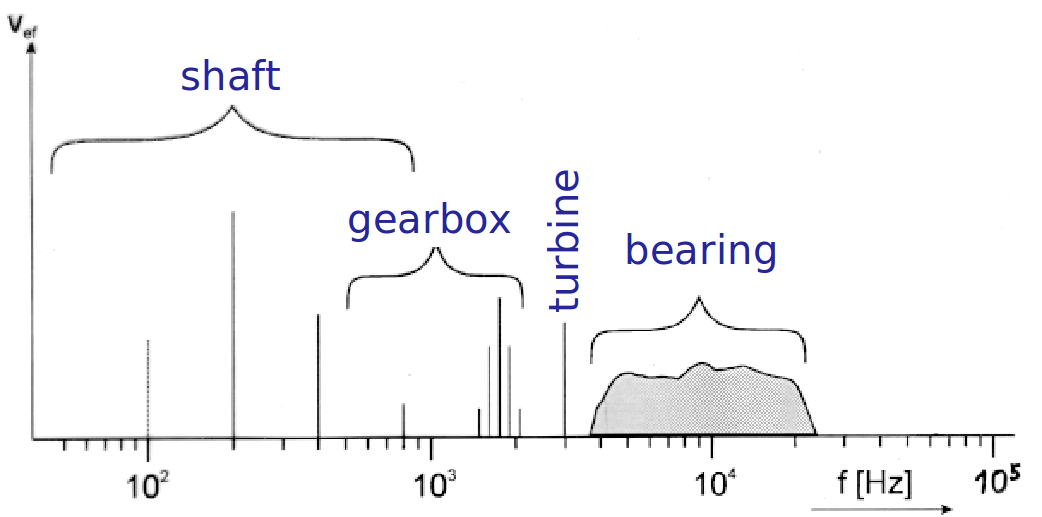
\includegraphics[width=0.85\textwidth]{DSP/Figs/vibrations.png}
    \end{figure} 

    
\section{Techniky zpracování signálu}
\label{section:techniky}
    Mnohé příznaky defektu motoru mohou být určeny přímo v tzv. časové oblasti signálu získaného z akcelerometru. Samotnému zpracování ale obvykle předchází určité předzpracování jako odstranění střední hodnoty a filtrace.\\
    Mocnějším nástrojem jsou poté techniky pracující se signálem ve frekvenční oblasti, které jsou z diagnostického hlediska mnohem komplexnější a poskytují informace o celkovém chování motoru. Motor je ze své podstaty periodické zařízení. Příznaky defektů ložisek se také periodicky opakují, a lze je proto detekovat ve spektru \cite{book:2}. Použití frekvenčních metod je úzce spojeno s~algoritmem FFT (Fast Fourier Transform) umožňujícímu efektivní získání spektra signálu.
    
\subsection{Techniky pracující se signálem v časové oblasti}
    
    \subsubsection{RMS (Root Mean Square)}
    Jednou z nejjednodušších analýz je výpočet efektivní hodnoty, která představuje kvadratický průměr a dobře popisuje celkovou sílu vibrací. Obecně platí, že se její hodnota zvyšuje s otáčkami stroje a pomocí jejího časového trendu dokážeme dobře detekovat větší defekty a opotřebení ložiska.
    \begin{equation}
        u_{RMS} = \sqrt{\frac{1}{N}\sum_{i=1}^{N} u[i]}, 
    \end{equation}
    kde $N$ je počet vzorků a $u_i$ je hodnota $i$-tého vzorku.
    
    
     \subsubsection{Krest faktor}
     \label{section:krest}
        Krest faktor je robustnější technika podávající informaci o impulsivnosti signálu. Obdélníkový nebo stejnosměrný signál má krest faktor roven jedné.\\
        Čím je tedy krest faktor vyšší, tím je signál impulsivnější. U běžných vibračních signálů motorů se krest faktor pohybuje mezi 2 a 6. Vyšší hodnoty obvykle indikují ostré nárazy uvnitř ložiska nebo motoru a obdobně jako u~RMS má krest faktor největší přínos při sledování jeho časového trendu.
        \begin{figure} [!h]
            \centering
            \caption{Časový průběh krest faktoru vzhledem ke změnám efektivní a maximální hodnoty napětí. Převzato z \cite{book:1}.}
            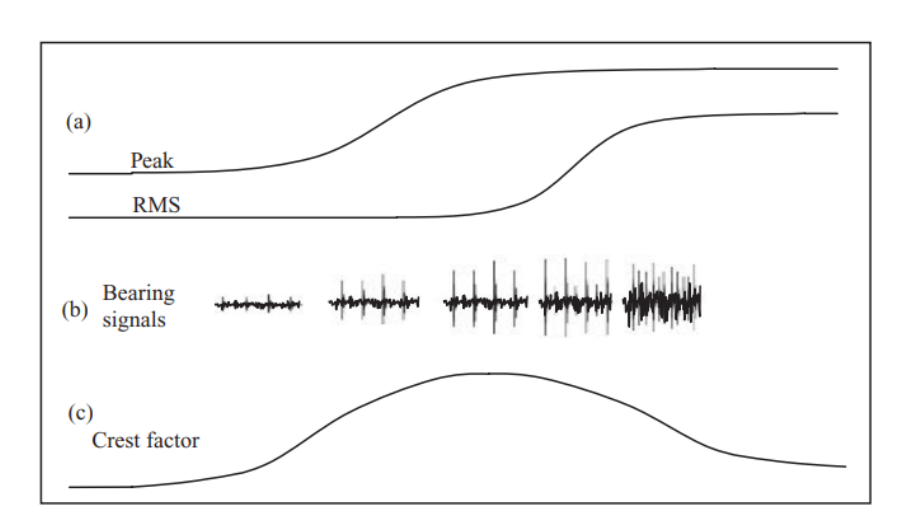
\includegraphics[width=0.8\textwidth]{DSP/Figs/krest_factor.png}
        \end{figure} 
        
        \begin{equation}
            CREST = \frac{|u_m|}{u_{RMS}}, 
        \end{equation}
        kde $u_m$ je maximální hodnota signálu a $u_{RMS}$ je efektivní hodnota.
  

    \subsubsection{Statistické momenty a Kurtosis Ratio}
    \label{section:kurtosis}
        Statistický moment je jednou z charakteristik pravděpodobnostního rozdělení. První a druhý moment je označován jako střední hodnota a variace, čtvrtý jako kurtosis (česky koeficient špičatosti). Pro vibrační analýzu je nejvýznamnější právě čtvrtý moment. Obecně platí, že nepoškozené ložisko vykazuje hodnoty kurtosis kolem 3, což odpovídá normálnímu rozdělení. Vyšší hodnoty poté mohou indikovat vadu \cite{book:2}.
        \begin{align}
            \mu = \text{E}\left[X\right] = \frac{1}{N}\sum_{i=1}^{N} x[i]\\
            \text{VAR}\left[X\right] = \sigma^2 = \text{E}\left[\left(X - \mu\right)^2\right]\\
            \text{KURT}\left[X\right] = \text{E}\left[\left(\frac{X - \mu}{\sigma}\right)^4\right]
        \end{align}
        
        Kurtosis Ratio je poté technika vyjadřující množství odchylek v signálu v~čase.
        Signál se nejprve ořízne, odstraní se z něj vychýlené hodnoty, tedy 5-10~\% největších a nejmenších hodnot (tato hodnota je přesně určena konfiguračním parametrem \texttt{dsp\_kurtosis\_trimmed\_samples}, více v kapitole \ref{section:config}) a spočítá se jeho kurtosis. Výsledkem je poté poměr kurtosis neoříznutého a oříznutého signálu. Pro signály, jež nevykazují vychýlené hodnoty (typicky obdélníkový signál), je kurtosis i po oříznutí stejná, a výsledek je tedy roven jedné \cite{article:2}.
        
        \begin{figure} [!h]
            \centering
            \caption{Oříznutí signálu pro výpočet kurtosis ratio. Převzato z \cite{article:2}.}
            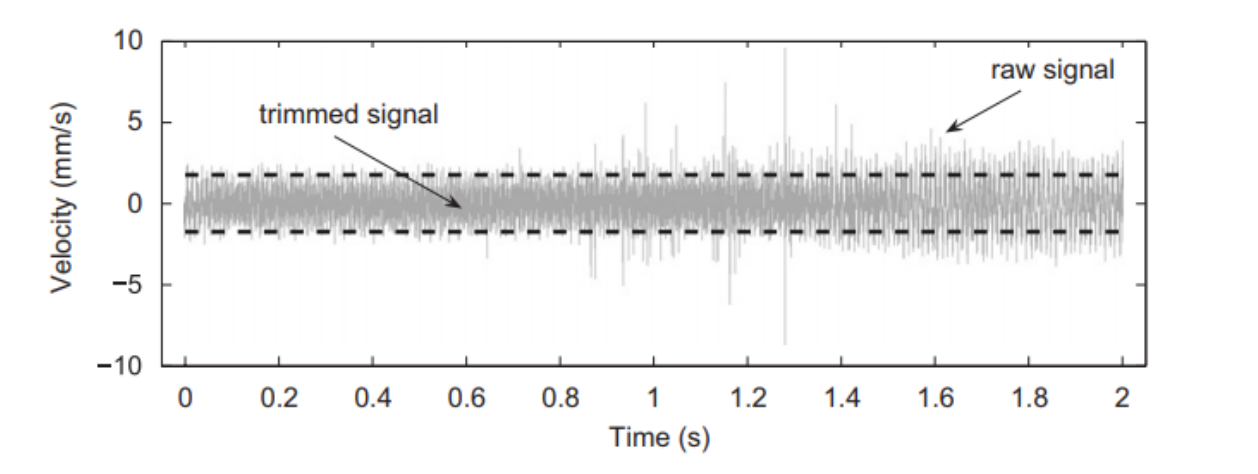
\includegraphics[width=\textwidth]{DSP/Figs/kurtosis_ratio.png}
        \end{figure} 
        
    \subsubsection{Starší, výpočetně nenáročné techniky}
        
        Následující tři techniky pocházejí z dávné minulosti, kdy AD převodníky nedosahovaly takových vzorkovacích frekvencí jako dnes a k zpracování signálu byl použit komparátor a čítač. Dnes se ale stále používají zejména u analýz velmi rychlých signálů jako jsou akustické emise s kmitočty kolem 10-1000~kHz. Především díky jejich výpočetní nenáročnosti a stále zajímavému informačnímu charakteru, který je v navržené aplikaci umocněn konfigurovatelností jejich parametrů – napěťové úrovně (konfigurační parametr \texttt{dsp\_voltage\_threshold}, více v kapitole \ref{section:config}), jsme se rozhodli, aby byly použity i v naší aplikaci pro analýzu vibrací.\\
        Jedná se konkrétně o tyto techniky, jejichž význam lze dobře vidět na obrázku \ref{figure:burst}.
       
        \begin{enumerate}
            \item \textbf{Ringdown Counts} – počet průchodů signálu předem určenou komparační napěťovou úrovní.
            \item \textbf{Rise Time} – doba náběhu signálu od prvního průchodu napěťovou úrovní po maximální hodnotu.
            \item \textbf{Signal Duration} – doba od prvního průchodu napěťovou úrovní po poslední průchod.
        \end{enumerate}{}
        
        \begin{figure} [!h]
            \centering
            \caption{Grafické znázornění technik využívajících komparační napěťovou úroveň. Převzato z \cite{website:8}.}
            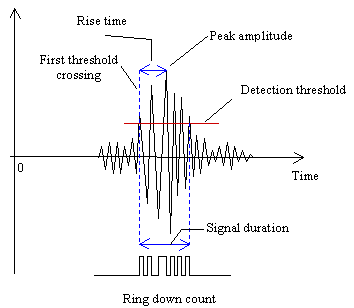
\includegraphics[width=0.8\textwidth]{DSP/Figs/burst.png}
            \label{figure:burst}
        \end{figure} 
        
        
    \subsection{Techniky pracující se signálem ve frekvenční oblasti}
    \subsubsection{FFT – amplitudové spektrum}
        Diskrétní Fourierova transformace signálu transformuje konečnou posloupnost jeho časově ekvidistantních $N$ vzorků do $N/2 +1$ dlouhé posloupnosti s~komplexními hodnotami odpovídajícími frekvenci \cite{book:2}.
        \begin{equation}
            X[k] = \sum_{n=0}^{N-1} x[n] e^{\frac{2\pi j}{N} k n}
        \end{equation}{}
    Výpočet DFT je algoritmicky náročný úkol – časová složitost $\mathcal{O}(n^2)$. Jeho realizaci na výpočetně slabších zařízeních umožňuje algoritmus FFT (Fast Fourier Transform), jehož časová složitost je $\mathcal{O}(n \log{}n)$. Implementace tohoto algoritmu byla převzata z DSP knihovny firmy ST Microelectronics \cite{software:1}.\\
    
    \begin{figure}[!hbp]
        \centering
         \begin{lstlisting}
            bool looksForMax = true;
    	    for (int i = 0; i < N/2; i++){
    	        //looks for max
        		if (looksForMax){   	
        			if (fftBuffer[i] > max)
        				max = fftBuffer[i]; maxPos = i;
        			else if (max - delta > fftBuffer[i]){
        			    --> Find minimum in saved peaks 
        			    and replace it {}
        				min = fftBuffer[i];
        				looksForMax = false;
        			}
        		}
        		//looks for min
        		else{                   
        			if (fftBuffer[i] < min)
        				min = fftBuffer[i];
        
        			else if (min + delta < fftBuffer[i]){
        				max = fftBuffer[i];
        				maxPos = i;
        				looksForMax = true;
        			}
        		}
    	}\end{lstlisting}
        \caption{Algoritmus pro vyhledávání extrémů amplitudového spektra.}
        \label{figure:algorithm}
    \end{figure}
    
    Díky použití sítě LoRa jako komunikačního média není možné odesílat celé amplitudové spektrum do centrální jednotky. Například pro 1024 vzorků by celková velikost paketů bez nákladů na režii protokolu měla velikost 2~KiB, což by z hlediska časových a energetických nároků bylo nerealizovatelné. Do centrální jednotky je tedy posláno pouze $k$ nejvýznamnějších extrémů, kde hodnota $k$~je jedním z konfigurovatelných parametrů – \texttt{fft\_peaks\_num} (více v kapitole \ref{section:config}).
    Graf $k$ nejvýznamnějších extrému, který je vygenerován ve webovém rozhraní lze vidět na obrázku \ref{figure:gui_other}. Celé amplitudové spektrum je možné zaslat do centrální jednotky pouze v debugovacím módu. Výstupem je graf, jehož příklad lze vidět například na obrázku \ref{figure:amplitude_01} získaném při experimentu.

    Na výběr $k$ nejvýznamnějších maxim ve spektru byl použit algoritmus pro hledání lokálních extrémů funkce \ref{figure:algorithm}.
    Míra selektivity extrémů ve spektru je ovlivněna parametrem delta, který je jedním z konfigurovatelných parametrů – \texttt{fft\_peaks\_delta} (více v kapitole \ref{section:config}).
    
   
    %   \begin{figure} [!h]
    %     \centering
    %     \caption{Ověření výpočtu – amplitudové spektrum reálné rotační soustavy při otáčkách 3000 RPM.}
    %     \includegraphics[width=0.7\textwidth]{DSP/Figs/3000_rpm_1khz_ok.png}
    %     \label{figure:spectrum}
    % \end{figure} 
    
 
    
    \section{Určení převodní konstanty}
        Z akcelerometru a AD převodníku získáváme údaj odpovídající pouze napětí. Pro jeho převod do jednotek odpovídajících zrychlení  – $\mathrm{m\,s^{-2}}$ nebo $g$ je třeba nalézt převodní konstantu.\\
        K tomuto úkolu byl využit referenční elektrodynamický budič vibrací (tzv. „shaker“) a přístrojový zesilovač NEXUS Conditioning amplifier s jednoosým přesným piezoelektrickým akcelerometrem s rozsahem 5000 $g$ \cite{manual:2}. Při použití obou akcelerometrů pro buzení motoru 400 Hz byla odečtena naměřená hodnota akcelerace na přípravku NEXUS a podle změřené efektivní hodnoty na použitém akcelerometru ADXL1002 vypočtena převodní konstanta.
        
        \begin{figure} [!h]
            \centering
            \caption{Přípravek NEXUS. Převzato z \cite{manual:2}.}
            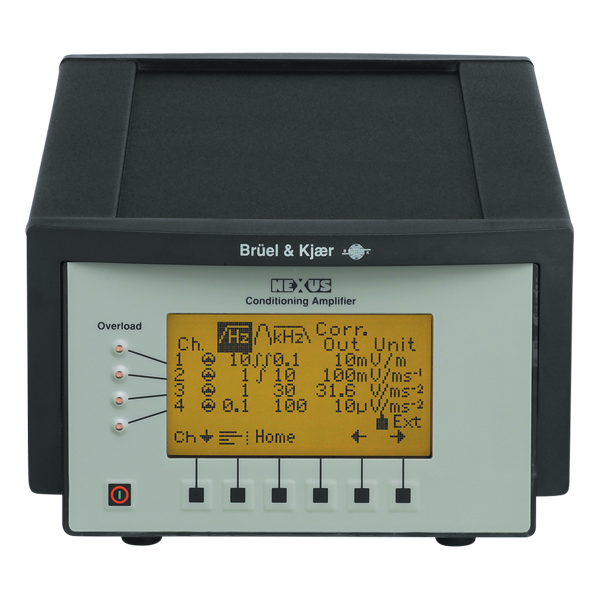
\includegraphics[width=0.5\textwidth]{DSP/Figs/nexus.png}
        \end{figure}       
        \begin{figure} [!t]
            \centering
            \caption{Výpočet převodní konstanty v laboratoři.}
            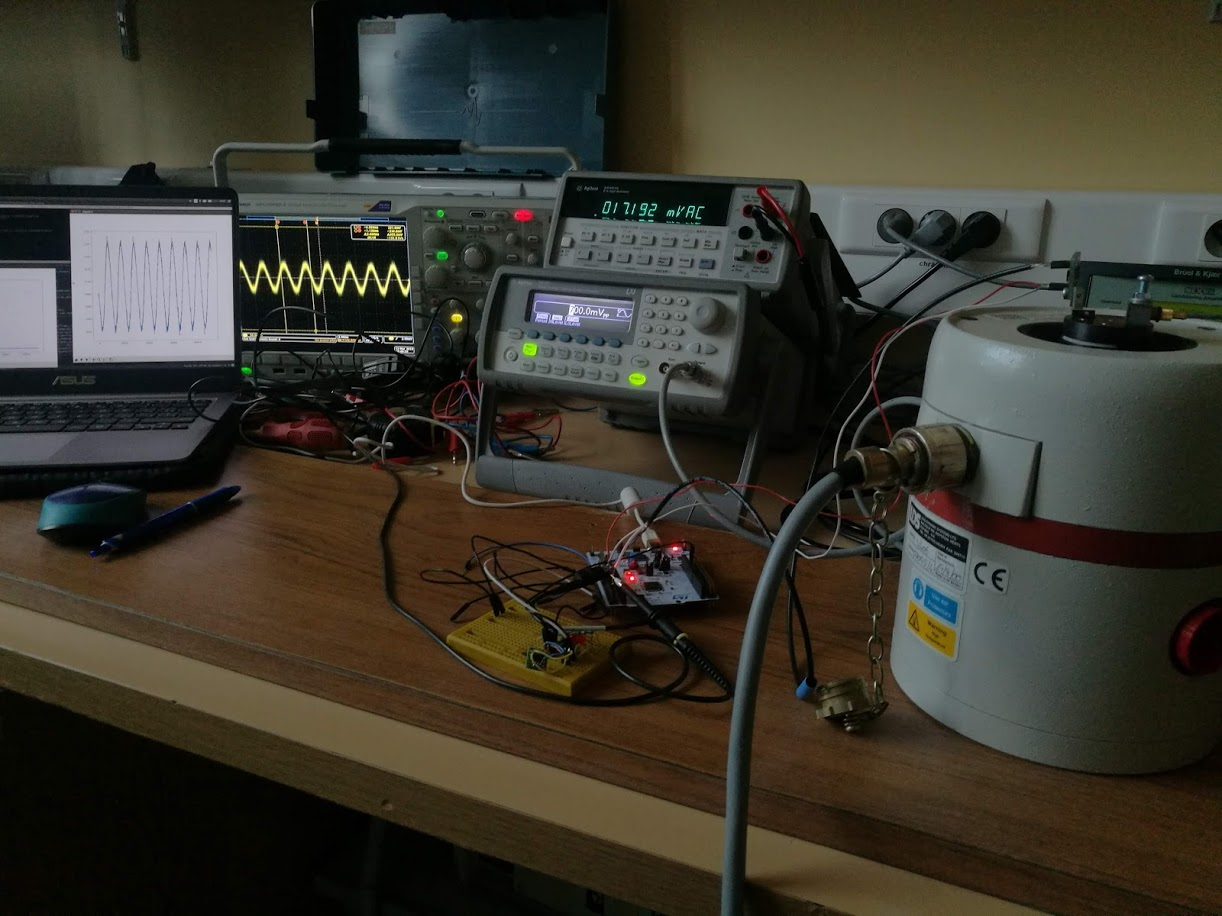
\includegraphics[width=\textwidth]{DSP/Figs/prakticka_zkouska.jpg}
        \end{figure} 
        
        
        
        

% ZDROJE 
% https://www.sczl.cz/download/download/2011-boretice/13-zkl-kotlan-vady-lozisek.pdf

% [55] S. G. Braun, Ed., Encyclopedia of Vibration. Elsevier, 2001.


% Kurtosis ratio
% J. Vass, R. Šmíd, R.B. Randall, “Avoidance of speckle noise in laser vibrometry by
% the use of kurtosis ratio: Application to mechanical fault diagnostics,” Mechanical
% Systems and Signal Processing, vol. 22, p. 647–671, 2008.
    
%CHECK ~
%CHECK red
%CHECK ...
\chapter{The Lighting System}
    In this chapter, a formal definition and introduction of all system parts with an explanation of their purpose is provided. The names for system devices used in the following chapters are \textbf{Light Control Unit} and \textbf{Floating Button}, and they were taken from SCILIF directly.
    Additionally, user and functional requirements and user interactions with the system are specified.
    
    \section{Light Control Unit}
        \label{sec:urs_lcu}
        The light control unit is a battery device connected directly to the optic fibres that are encased in textile clothing. The brightness emitted by optic fibres is set by controlling the electrical current flowing through optical LED powering a light guide. There are several pre-defined levels of brightness and blinking modes called light modes (see section \ref{sec:light_modes}).
        The unit is usually placed in a pocket typically located at the back waist part of a vest or a jacket.
        
        \begin{figure}[!ht]
            \centering
    	    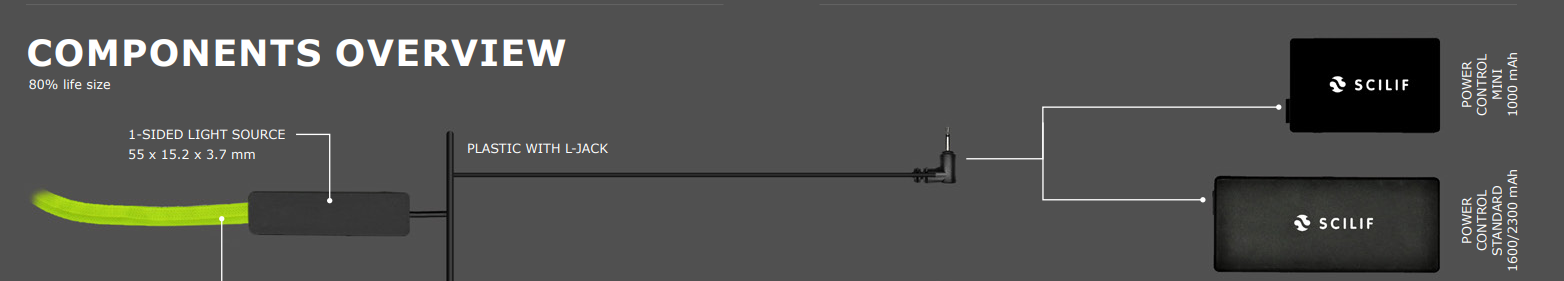
\includegraphics[width =1.1\textwidth]{URS/Figs/scilif_system01.png}
            \caption {A visualization of the light control unit}
            \label{figure:scilif_lcu}
        \end{figure}  
        
        
    \section{Floating Button}
        \label{sec:urs_fb}
         The floating button is a battery device placed on a comfortably reachable part of a vest/jacket. It allows the user remotely and quickly change the light modes on the light control unit without the need to open the smartphone/smartwatch application. Because the floating button communicates with the light control unit remotely, no connection cables are needed. Furthermore, the floating button is designed to have good haptic properties. 
       
        \begin{figure}[!ht]
            \centering
    	    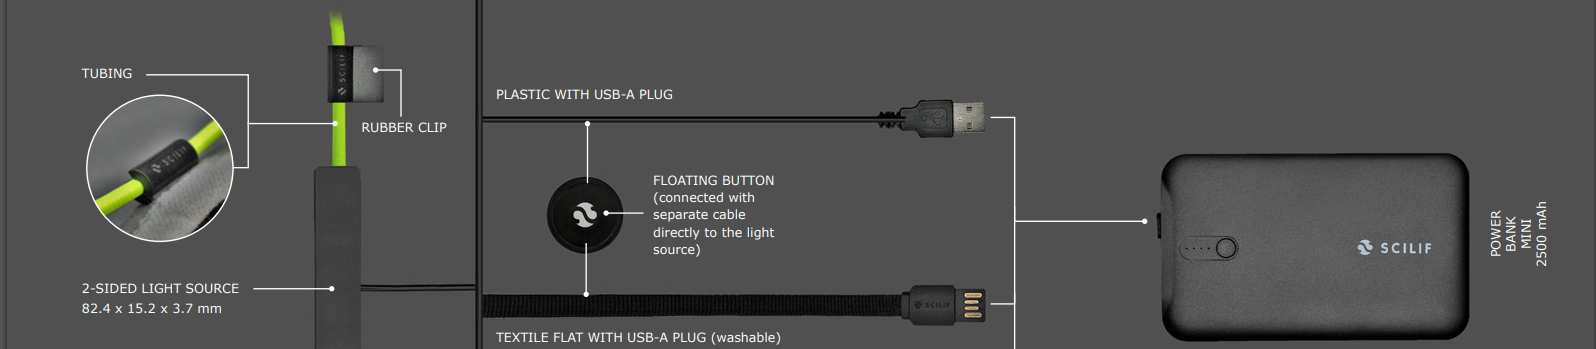
\includegraphics[width =1.1\textwidth]{URS/Figs/scilif_system02.png}
            \caption {A visualization of the floating button}
            \label{figure:scilif_fb}
        \end{figure}  
       
    \section{RFID Switch}
        The RFID switch consists of two parts - RFID reader and RFID tag. Both of them can be sewed into the clothing - the coil of RFID reader into arbitrary comfortably reachable part and the RFID tag into a sleeve. When the user wants to change the light mode, he only needs to bring the sleeve near the coil to trigger the light mode change. Due to the fact that the RFID reader has to be physically connected to the light control unit, wires must be stitched onto the clothing. 
       
       
    \section{Light Modes}  
    \label{sec:light_modes}
        As the most important user interaction with the system, the light control unit allows turning on/off the lighting or changing the predefined light modes. At the time of writing, five different light modes were defined:
        
        \begin{enumerate}
            \item No Lighting 
            \item Strong Lighting (145 mA)
            \item Low Lighting (60 mA)
            \item Slow Blinking (2 s period)
            \item Fast Blinking (0.5 s period).
        \end{enumerate}
        
        Both blinking modes use strong lighting (145 mA), and the duty cycle is 50 \%. These numbers were defined according to SCILIF requirements.
        
        The state of the art of this problem is to develop a satisfying way how to change these light modes. The considerations were given on how practical and comfortable the solution is, as well as on meeting the client's functional requirements, such as maintaining low power consumption, reducing the additional costs, etc. 
       
       \subsection{Methods for changing the light modes}
        \label{sec:light_modes_methods}
        
        During the work on the thesis, multiple ways how to change the light modes were implemented. The direct change to preferred light mode is possible only through mobile/smartwatch application. All other methods simply increment the current mode.
        The list below shows all of them.
        
        \begin{itemize}
            \item Pressing button on the light control unit
            \item Remote change over BLE by mobile/smartwatch application
            \item Remote change over BLE by tapping on the floating button
            \item RFID switch
            \item Gesture control (not implemented yet) 
        \end{itemize}
        

        Since the spectrum of end-users is large, particular methods might suit different customer needs or use cases. The most relevant questions that should be addressed are: \\
        
        \begin{itemize}
        \setlength\itemsep{0em}
            \item  How to change the light mode when the unit is not reachable by hands. The unit might be encased in the clothing, or it might be located in the back pocket. \\
            \item How to change the light modes quickly, with the least possible effort (for example, in the case of a motorbike driver or a biker). 
        \end{itemize}
        
        
        A quick analysis of these methods:
        
        \textbf{Change by pressing the button on the light control unit directly} brings no overhead in terms of costs and battery usage. Nevertheless, it is the less practical method, and in many use cases, it is not applicable at all.
        
        \textbf{Remote change by mobile/smartwatch application} is based on BLE communication between the central (mobile phone/smartwatch) and peripheral (light control unit). Initially, the light control unit needs to be bonded and connected to the central.\\
        The advantage of this method is that it allows changing the light modes even though the unit is not reachable. On the other hand, one still needs to take a mobile phone and open the mobile application, so it is not very practical in the use cases when a quick change is desired. This method also increases the overall cost and battery consumption since a BLE-based MCU must be used.
        
        \textbf{Change by RFID switch} is based on the inductive coupling principle. When the user brings the sleeve with encased RFID tag close to the reader, it triggers the change of a light mode.\\
	    This method addresses both questions defined above. On the contrary, the biggest drawback of this method is the increased battery consumption needed for checking the incoming RFID transmissions. Besides that, the cables between the coil of RFID reader and the unit must be sewed into the clothing and the probability of unwanted switches increases.
        
        \textbf{Remote change by tapping on the floating button} is based on BLE communication between the central (floating button) and the peripheral (light control unit). The light control unit needs to be bonded and connected to the central.\\
        Apart from solving both constraints defined above, this method also does not require any wiring. Nevertheless, it brings the biggest overhead in terms of the costs since two BLE devices must be used.
        
        \textbf{Change by a gesture} allows the user to change the light mode by a predefined gesture. It is rather an experimental feature.
        
        
        Last but not least, one should take into account that these methods could be combined, and it always depends on the use case and customer's preferences.
        
    \section{Maintenance}
       Considering the fact that both the light control unit and floating button are battery devices, the system should be able to provide information such as battery level,  charging status or temperature. These so-called maintenance data can be obtained via BLE using a mobile/smartwatch application.

        Another user's interaction with the system is the OTA (Over The Air) firmware upgrade that enables users to flash a new firmware version through a mobile application over BLE.

        Both of these are possible only with BLE-based MCU.
        
        
        
        
%!TEX ROOT=ctutest.tex
\chapter{HW Specification}
    This chapter serves as a description of hardware components used in the system. Attention will be given to the technical details of specific components and the reasons behind choosing them.
    
\section{HW of Light Control Unit}
    The light control unit board is based on the nRF52833 BLE SOC (System on Chip) from Nordic Semiconductor. The board also contains a stabilizer circuit, charger circuit, USB-C connector, three small RGB LEDs for signalization and one push button.\\
    Another part is a step-up converter based on the DIO5661 chip with SEPIC (Single-ended Primary-inductor Converter). This PWM to constant current converter controls the electrical current in optic fibres - the board is connected to them through 2.5 mm jack.
    
    Finally, the board also contains an accelerometer/gyro LSM6DSMTR and a microphone. 
    The 1600mAh 3.7V Lithium-ion rechargeable battery is soldered directly on the PCB and needs to be connected with a jumper. To increase the reach, a Molex 2.4/5 GHz antenna can be connected as well. 

    \subsection{Microcontroller (MCU)}
        The nRF52833 is general-purpose multi-protocol SOC (System On Chip) device supporting not only BLE but also Zigbee, Bluetooth Mesh and NFC.
        
        \begin{figure} [!hb]
    	    \centering
    	    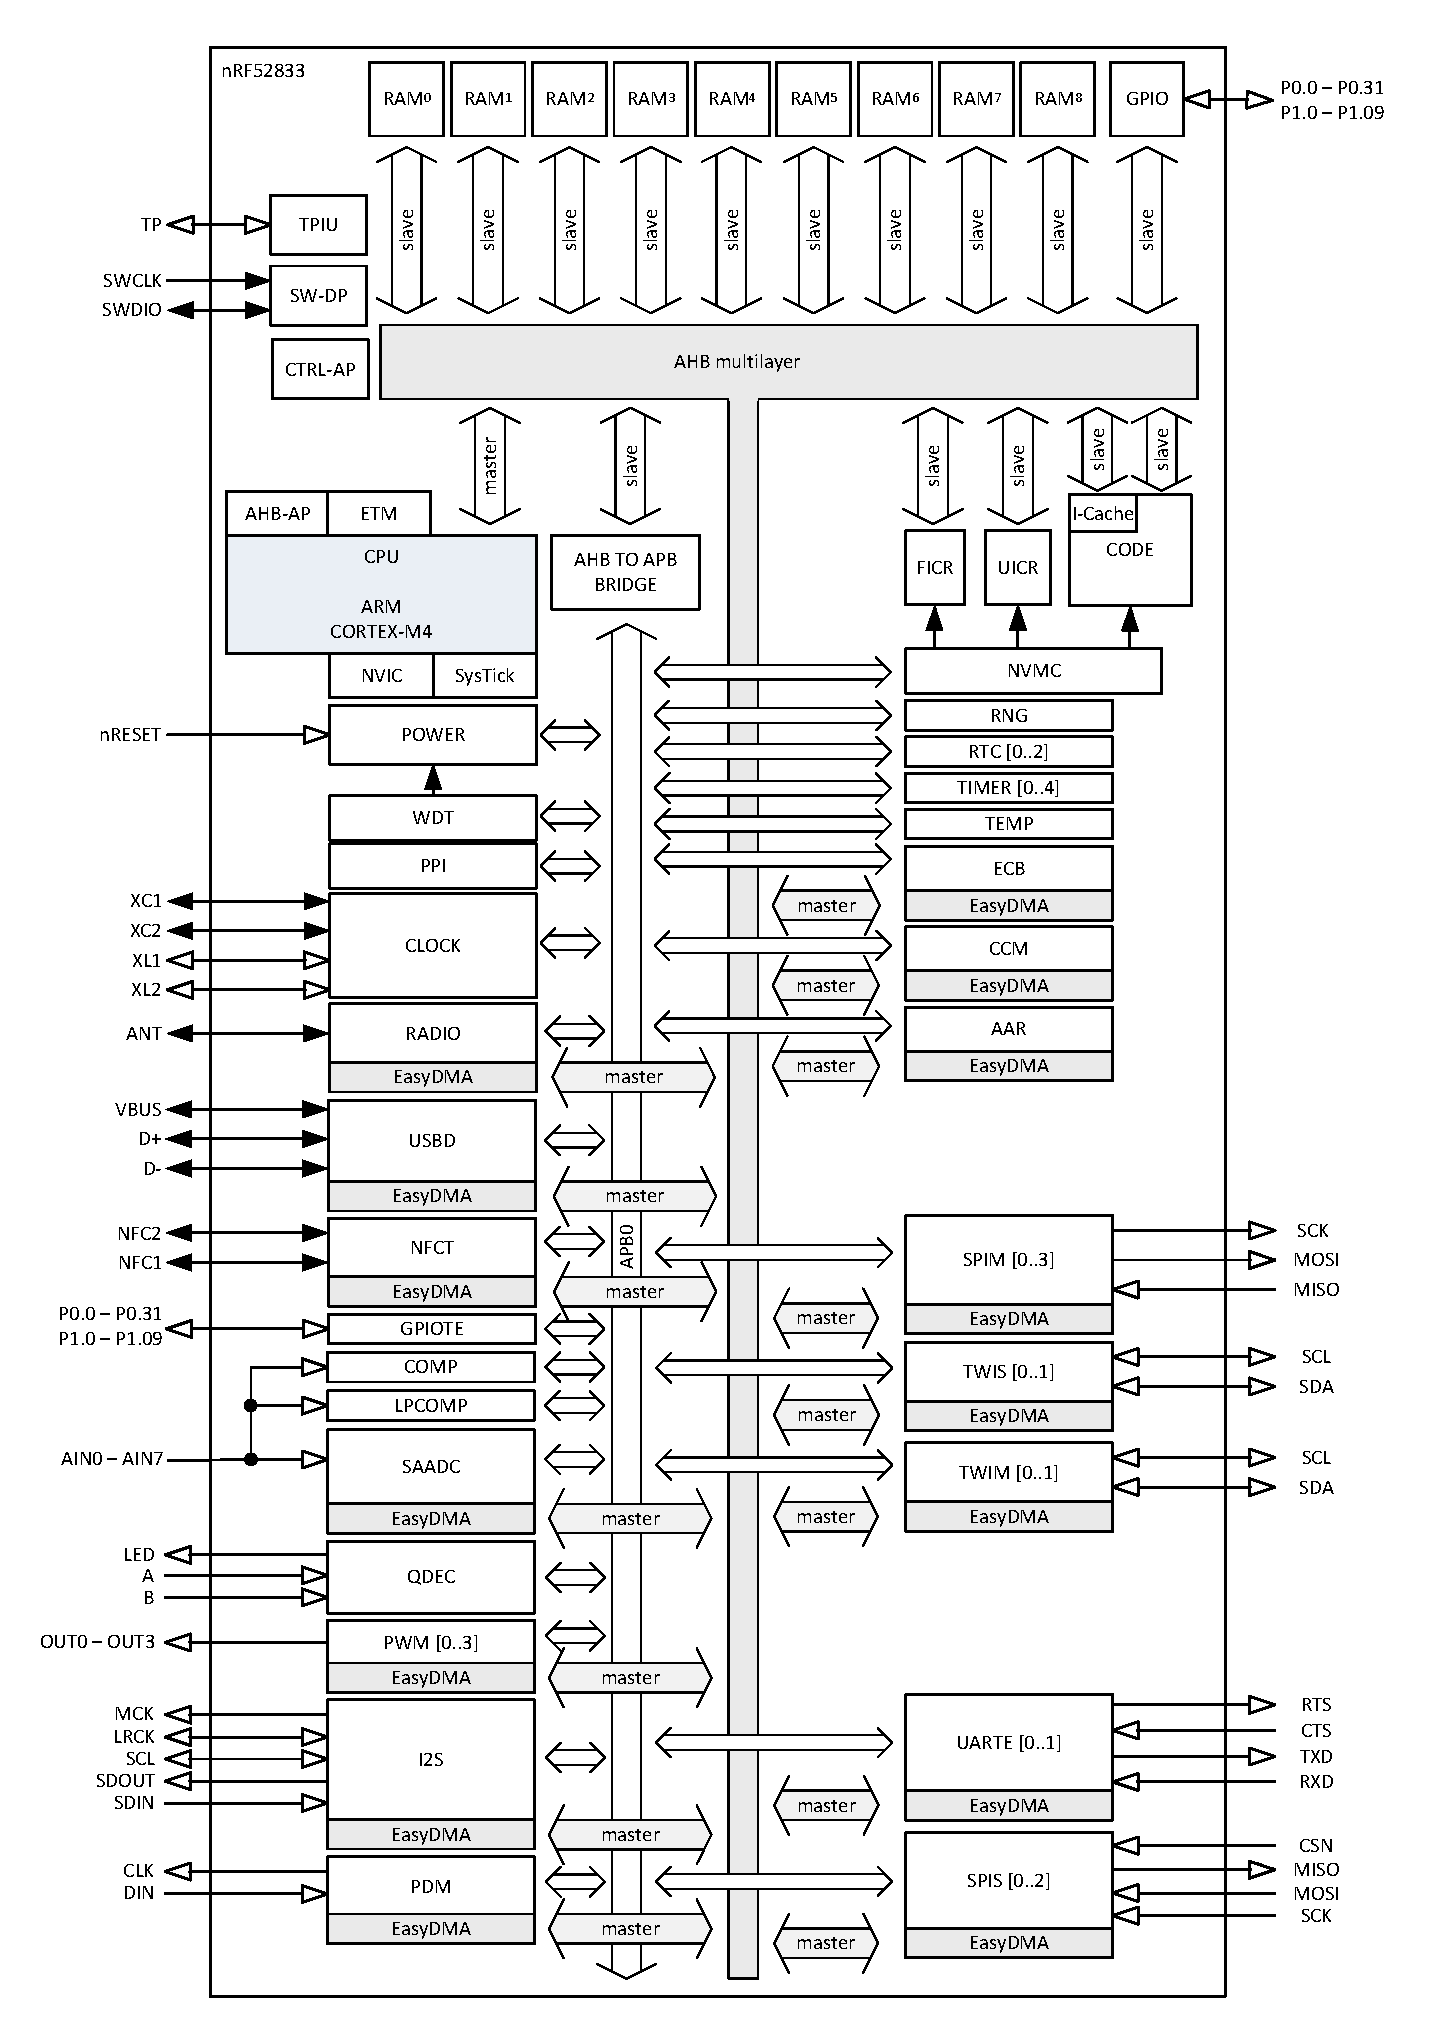
\includegraphics[ width =0.8\textwidth]{02.HW/Figs/nrf52833_blockdiagram.pdf}
            \caption {nRF52833 block diagram (taken from \cite{image:nrf52833_block_diagram})}
        \end{figure} 
        
        
        \begin{titleitemize}{Specification of nRF52833 with selected peripherals:}
            \item 32-bit RISC ARM Cotex M4 with FPU, 64 MHz 
            \item 512 kB flash and 128 kB RAM memory 
            \item HFCLK from 64 MHz on-chip oscillator / 32 MHz external oscillator, LFCLK from 32 kHz RC oscillator 
            \item 42 GPIO pins
            \item 12-bit ADC 200 ksps, 8 channels 
            \item 4x PWM, 4 channels
            \item 2x UART, 4x SPI, 2x $\text{I}^2\text{C}$
            \item 5x 32-bit timer with counter mode, 3x RTC counter
            \item temperature sensor
        \end{titleitemize}
        \newpage    
        
            \begin{titleitemize}{Power Management:}
                \item Power consumption in SYS-OFF mode:  \SI{0.6}{\micro\ampere} (at 3V)
                \item Power consumption in SYS-ON mode (IDLE):   \SI{1.5}{\micro\ampere} (at 3V)
                \item 4.9 mA peak current in TX (0 dBm)
                \item 4.6 mA peak current in RX
            \end{titleitemize}
        
        
        \subsubsection{PPI}
        \label{sec:ppi}
             PPI (Programmable Peripheral Interconnect) is an advanced chip's interface that allows peripherals to connect and communicate with each other using a system of tasks and events without the need of the MCU. It becomes beneficial especially when precise synchronization between events and tasks is needed (for example, sampling).
        
        \subsubsection{EasyDMA}
            EasyDMA is easy to use Direct Memory Access that provides some peripherals with direct access to the RAM without the need of the MCU. Multiple DMA instances for a peripheral are allowed, so writing to the RAM and reading from it is possible simultaneously.
        
        
        \subsubsection{ADC}
            The successive approximation analog-to-digital converter supports up to eight external input channels (8 single-ended inputs or 4 differential inputs) in 8/10/12 bit resolution.
            
            Each ADC channel can use an individual voltage reference - either the 0.6 V internal reference or VDD/4. Using the VDD based reference is useful if the measured signal fluctuates depending on VDD.
            
            The maximum sampling frequency is 200 kHz (inverse value of summation of conversion time - $t_{conv} = \SI{2}{\micro\second}$ and minimum acquisition time - $t_{acq} = \SI{3}{\micro\second}$. The acquisition (sampling) time determines how long the channel input is connected to the external source. 
            
            % The simplified scheme of nRF52 ADC:
                
    \subsection{Radio}
        The 2.4 GHz transceiver is integrated on the nRF52833 chip. It supports multiple radio standards such as 1/2 Mbps BLE modes, long range 250/500 kbps BLE modes or IEEE 802.15.4 based 250 kbps mode (LR-WPAN). Besides that, it also implements the Bluetooth direction finding.
        
        The radio uses DMA for reading and writing data packets from and to the RAM without CPU involvement. Apart from that, it involves an automated packet assembler, packet disassembler, automated CRC generator and CRC checker.
        
        % \textbf{Specification of radio:}
            \begin{titleitemize}{Specification of radio:}
                \item 1 and 2 Mbps BLE modes
                \item 250 and 500 kbps long range BLE modes 
                \item IEEE 802.15.4 250 kbps mode (LR-WPAN)
                \item -96 dBm sensitivity in 1 Mbps BLE mode
                \item -103 dBm sensitivity in 125 kbps BLE mode (long range)
                \item -20 to +8 dBm TX power, configurable in 4 dB steps
            \end{titleitemize}
            
            \begin{figure} [!ht]
        	    \centering
        	    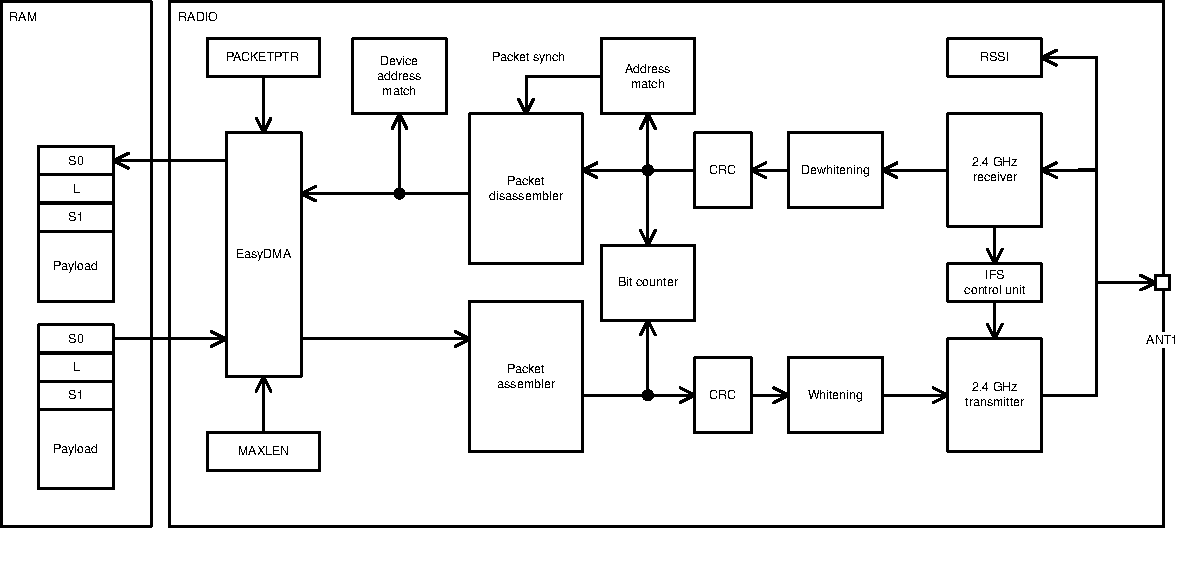
\includegraphics[ width =1.05\textwidth]{02.HW/Figs/nrf52833_radio.pdf}
                \caption {nRF52833 radio block diagram (taken from \cite{image:nrf52833_radio_block_diagram})}
            \end{figure} 
                

     
    \subsection{Gyroscope/Accelerometer}
        \todo{TO BE DONE ...}
        
        % The choice of LSM6DSMTR accelerometer/gyro was determined mostly by...
        % \textbf{Specification:}
    
    % \subsection{SEPIC}
        
        %     \todo{Provide some theoretical background/calculations to SEPIC circuit}
    
    
    \subsection{The Overall Design}
        The first version of the hardware of the light control unit was designed by Pavel Porazil from PiKRON company during summer 2021 (the whole scheme is in appendix - \ref{figure:hw_lcu}). The case for the unit and the sticker comes from SCILIF company directly.
        
        \begin{figure} [!ht]
    	    \centering
    	    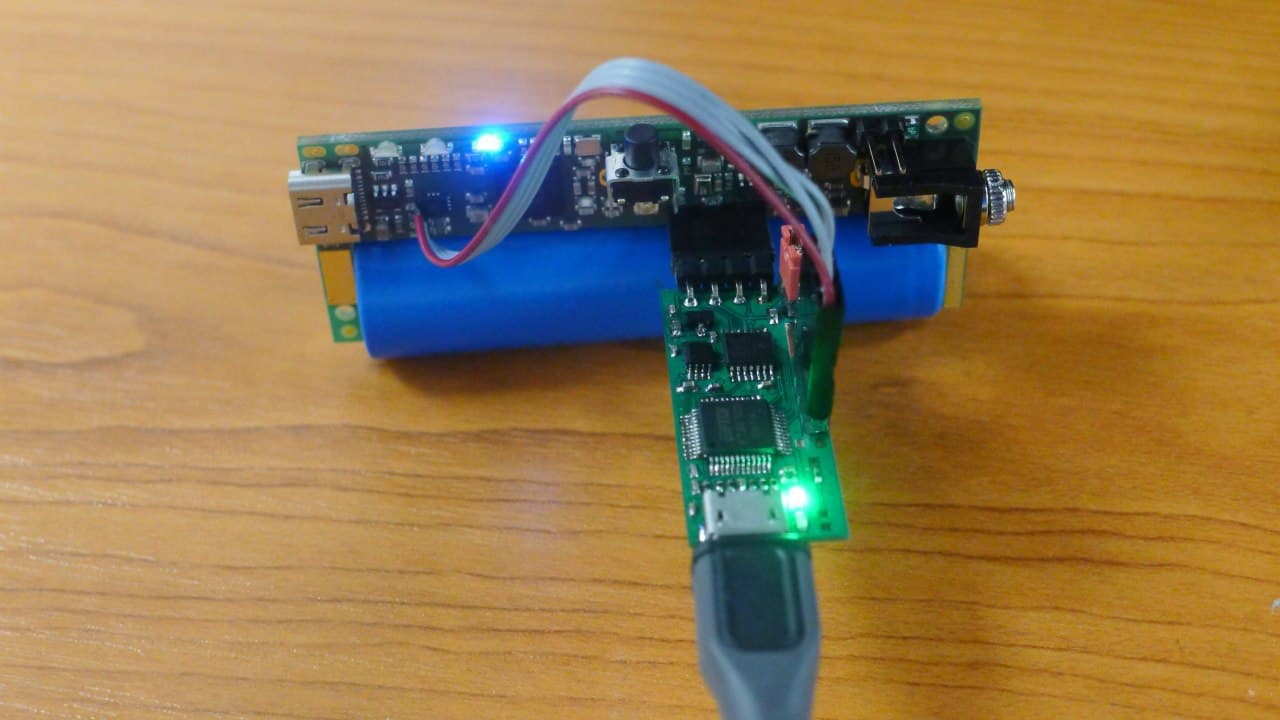
\includegraphics[ width =0.8\textwidth]{02.HW/Figs/overall_unit.jpg}
            \caption {Light Control Unit board from Pavel Porazil with PiKRON programmer}
        \end{figure} 
    
\section{HW of Floating Button}
    For the first prototype of the floating button, the development board BBC micro:bit.v2 was selected. The fact that the board is based on the nRF52833 as well helped significantly during programming.
    
    The board also comprises LED matrix of 25 LEDs, two push buttons, a micro-USB connector, two signalization LEDs, a microphone, speaker, touch sensor and accelerometer/magnetometer LSM303AGRTR. 
    
        \begin{figure} [!ht]
            \centering
            \caption{BBC micro:bit.v2 (taken from \cite{image:BBC_microbit})}
            \begin{subfigure}[b]{0.48\textwidth}
                 \centering
                 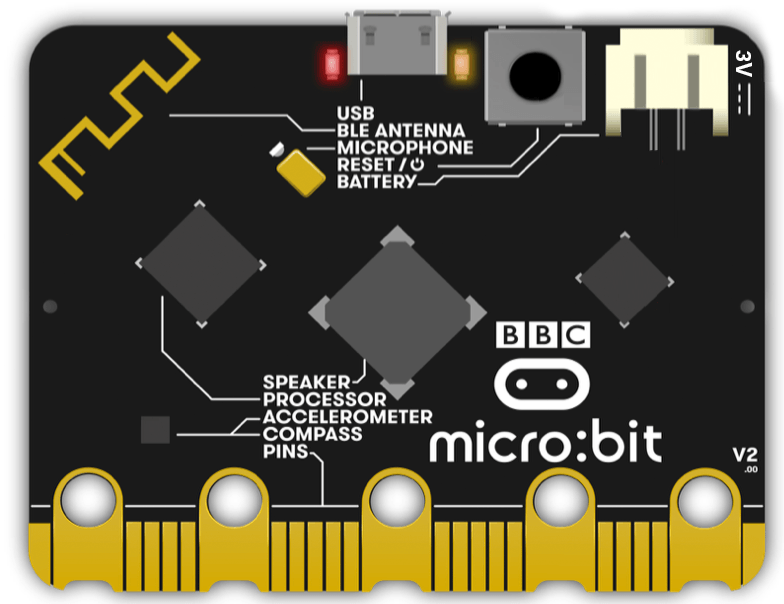
\includegraphics[width=\textwidth]{02.HW/Figs/microbit.png}
             \end{subfigure}
             \hfill
            \begin{subfigure}[b]{0.45\textwidth}
                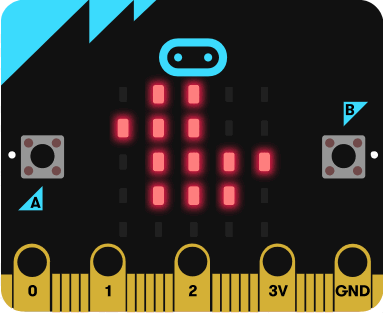
\includegraphics[width=\textwidth]{02.HW/Figs/microbit3.png}
            \end{subfigure}
        \end{figure}     
        
    \subsection{Accelerometer/Magnetometer}
        \todo{TO BE DONE...}
        % \textbf{Specification:}


\section{HW of RFID Switch}
    \label{sec:hw_rfid_switch}
     The RFID switch consists of an active reader and a passive tag. The RFID reader can be integrated as a part of the light control unit board or connected and powered externally. In both cases, the coil (antenna) must be wired to the reader. 
    
    \subsection{RDM6300 RFID Reader}
        \label{sec:hw_rfid_rdm6300}
        As a first prototype of the RFID reader, the development module RDM6300 was chosen. RDM6300 is a LF RFID reader designed to read data from 125 kHz, EM4100 compatible tags using a RF receiver circuit and built-in MCU. An external antenna needs to be connected to the board directly.
        The RDM6300 uses demodulation and decoding algorithms and only transmits the received bits over a serial communication (UART) at a 9600 baud rate.\\
        The whole module was connected to the light control unit through a few jumper wires.
        
        
        % \textbf{Specification of RDM6300:}
        \begin{titleitemize}{Specification of RDM6300:}
            \item 125 kHz operating frequency 
            \item 20-50 mm receive distance
            \item around 50 mA working current
            \item 5V working voltage
        \end{titleitemize}
            
        \begin{figure} [!ht]
            \centering
            \caption{EM4100 RFID tag and RDM6300 RFID reader (taken from \cite{image:em4100}, \cite{image:rdm6300})}
    
            \begin{subfigure}[b]{0.45\textwidth}
                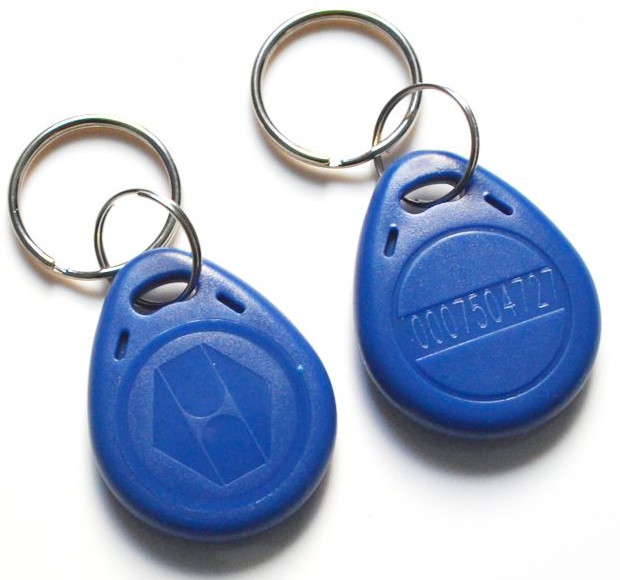
\includegraphics[width=\textwidth]{02.HW/Figs/em4100.jpg}
            \end{subfigure}
             \hfill
            \begin{subfigure}[b]{0.45\textwidth}
                 \centering
                 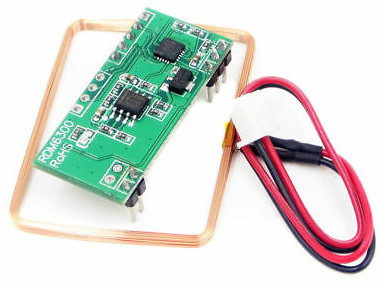
\includegraphics[width=\textwidth]{02.HW/Figs/rdm6300.jpg}
             \end{subfigure}
        \end{figure}     
             
        
            
    \subsection{Custom Low Power RFID Reader}
        The main drawback of the RFID reader lies in a high standby current consumption (around 50 mA). A custom low power RFID reader circuit was designed to mitigate this problem \ldots
        
        \todo{TO BE DONE...}
        
    \subsection{EM4100 RFID Tag}
        The RFID tag in a key fob form is based on a cheap EM4100 chip made by the company EM Microelectronic. 
        The 64 bits of data are read-only, factory preprogrammed,  and represent a unique identifier of the tag, which is also printed on the PVC, so it can not be changed. \\
        The RFID reader must know how the data is stored in the tag and which protocol to use to extract it - demodulation and decoding method.
        

% \section{Additional Fast thoughts}
%     The solution has been use only with specific SCILIFF


\todo{Include analyisis of current BLE based MCUs}

\todo{Provide some theoretical background to SEPIC}



%!TEX ROOT=ctutest.tex

\chapter{Software Development - Firmware}
    In this chapter, a comprehensive analysis of software development tools and techniques is provided. The first sections \ref{sec:fw_tools_used} - \ref{sec:fw_memory_layout} generally describe the process of development on nRF52833. The mutual aspects (BLE properties and application logic) of both the light control unit and floating button are analyzed in section \ref{sec:app_ble} and \ref{sec:app_businnes_logic}. The following two sections focus on each device individually, showing their application state diagrams. In the last sections \ref{sec:fw_rfid} - \ref{sec:ota}, a detailed description of pertinent system parts is given - such as button clicks debouncing, OTA upgrade or RFID control.
    
    
    
\section{Tools Used}
    \label{sec:fw_tools_used}
    The firmware was written in C language with the help of Nordic SDK.
    The SDK includes various drivers, libraries, examples and most importantly, a SoftDevice, a BLE protocol stack provided as a precompiled and linked binary file \cite{nrf52doc:softdevice}. The SoftDevice types differ in complexity and performance (for instance, the maximum number of concurrent links they can handle or the BLE role they support etc.). The light control unit and floating button are based on the SofDevice \textbf{S132} and \textbf{S140}, respectively. 
    
    Apart from SoftDevice, the HAL libraries (called NRFX), some additional middle-layers (RTC based timer/scheduler), utilities (logging module) and the BLE middle-layers were incorporated into the project. A crucial role plays, for instance, a peer-manager library which provides a whole infrastructure to security management and cryptography operations.
    
    \subsection{Programming}
        The programs are flashed to targets through OpenOCD (Open On-Chip Debugger), which uses a built-in SWD adapter on the microbit board and an external programmer on the light control unit board to communicate with the nRF52 chip.\\
        OpenOCD complies with a remote gdbserver protocol, and therefore, gdb (GNU Debugger) with a graphical user interface DDD (Data Display Debugger) was used for applications debugging.
        
        To flash all software parts at once (SoftDevice, application and bootloader - see section \ref{sec:fw_memory_layout}), a python script \verb|merge_hex| was written that merges all three .hex files and converts them to a binary form.\\
        An additional, python-based tool called \verb|nrfutil| provided by Nordic directly allows generating specific bootloader settings and creating an initialization packet for DFU upgrade - see section \ref{sec:dfu_process} for a detailed description.
   
   
    
\section{nRF52 Memory Layout}
\label{sec:fw_memory_layout}
    This section briefly introduces the memory layout of nRF52 and shows where all parts of device firmware (SoftDevice, application and bootloader) are flashed.

    \begin{figure} [!ht]
	    \centering
	    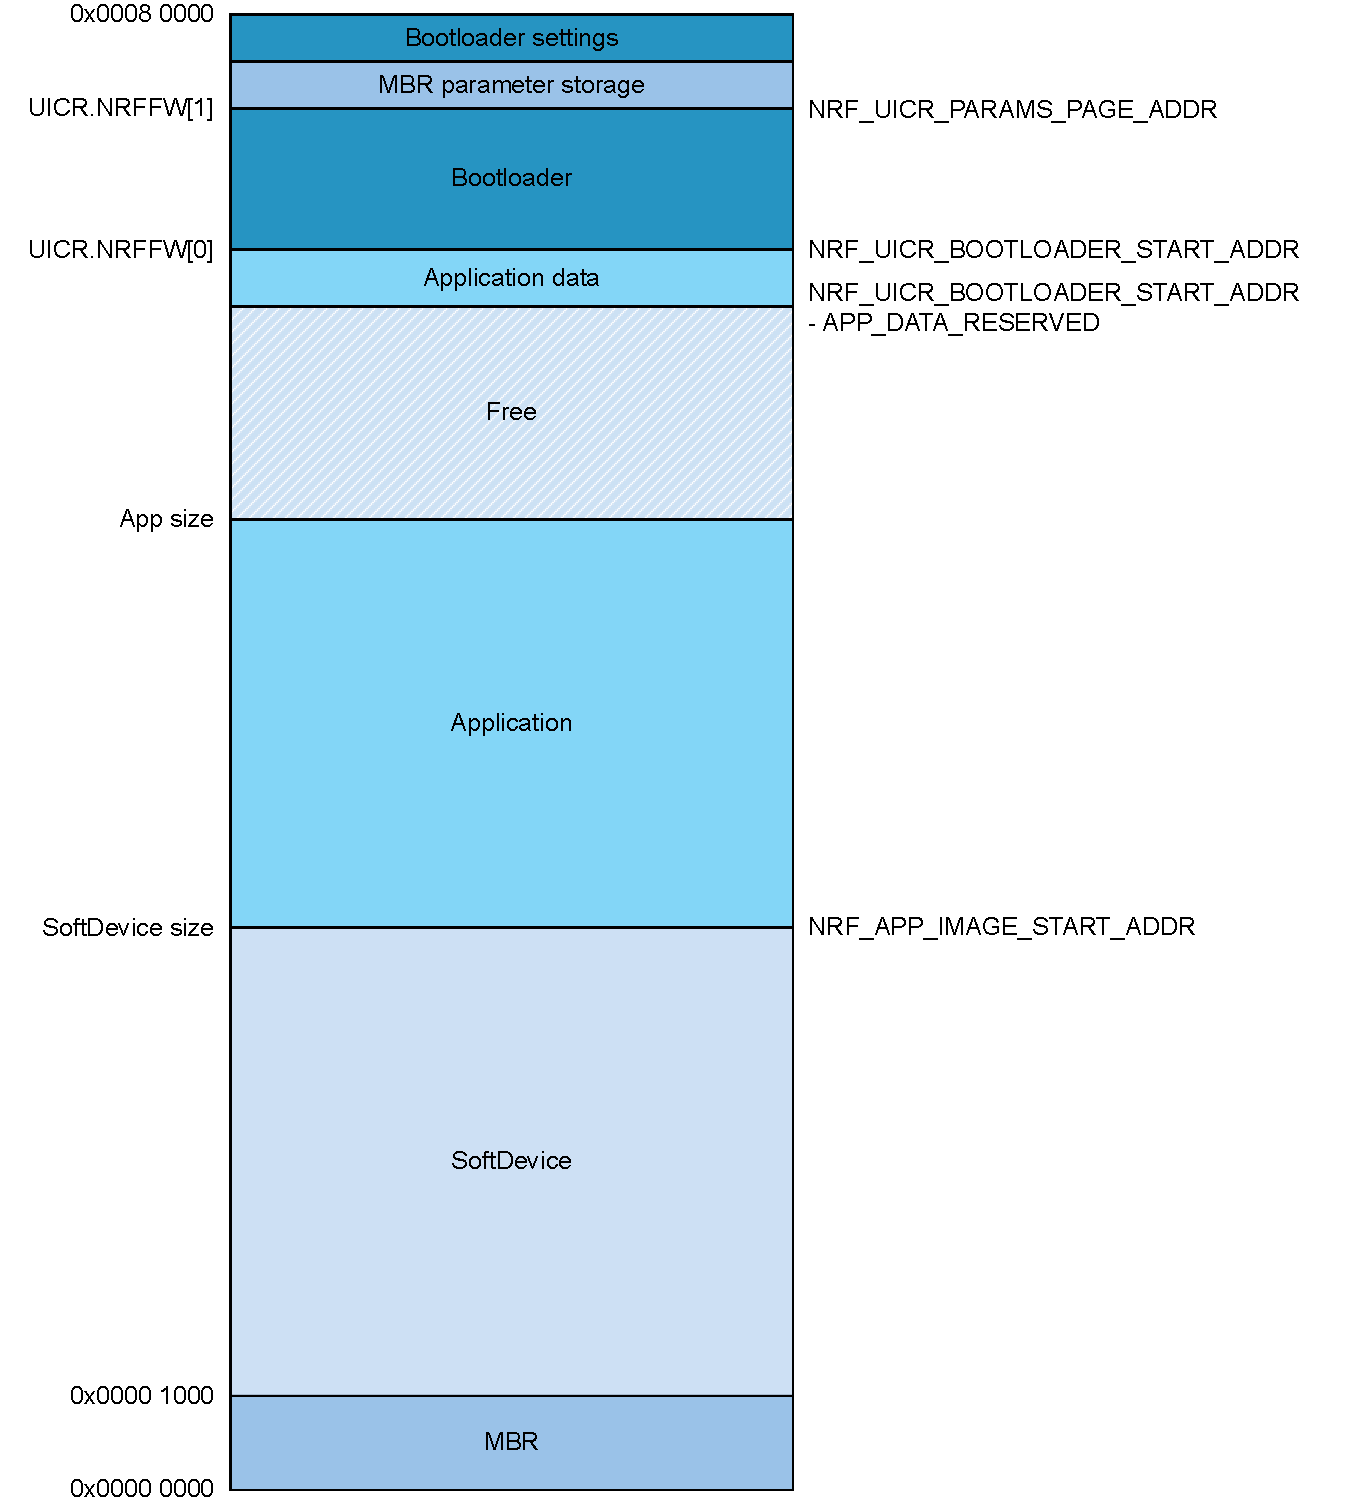
\includegraphics[ width =0.75\textwidth]{SW_Firmware/Figs/nrf52_memory.pdf}
        \caption {nRF52 memory regions (taken from \cite{image:nrf52_memory_layout})}
        \label{figure:fw_memory_layout}
    \end{figure}  
    

    \textbf{MBR (Master Boot Record)}\\
        The MBR table is a part of the SoftDevice and it occupies 4 kB of memory at addresses 0x0000 - 0x1000. Its primary function is to provide an interface for system-in updates, ensuring the continuity of DFU upgrades in case of power loss. It also contains the System Vector table, so all interrupts are at first processed by MBR and then forwarded to the bootloader or SofDevice \cite{nrf52doc:softdevice}.
    
    \textbf{SoftDevice}\\
        SoftDevice is in charge of the low-level BLE communication. The amount of occupied memory depends on the SoftDevice type. Each SoftDevice includes a predefined hardcoded start address of the application where it jumps \cite{nrf52doc:softdevice}. 
        
    \textbf{Application}\\
        The application address space starts from a predefined address determined by SoftDevice type - \sss{NRF\_APP\_IMAGE\_START\_ADDR} and ends at the start of the bootloader -  \sss{NRF\_UICR\_BOOTLOADER\_START\_ADDR} \cite{nrf52doc:bootloader}.
    
    \textbf{Bootloader}\\
        A bootloader is a minimal piece of code responsible for booting into the application or entering a DFU mode. While in DFU mode, it enables receiving and processing wireless firmware updates - see section \ref{sec:ota} about OTA.\\ 
        If the bootloader start address is present at UICR (User Information Configuration Register) in non-volatile memory, the MBR boots the bootloader instead of SoftDevice \cite{nrf52doc:bootloader}.
        
    \textbf{Bootloader Settings}\\
        A bootloader settings page occupies 4 kB of flash at address 0x7E000, and it contains information about the current DFU process and the metadata about the installed application, such as firmware and hardware version \cite{nrf52doc:bootloader}.
    
    \textbf{MBR Params Page}\\
        The last 4 kB of flash is dedicated to MBR parameters. It stores the state information of flash operations or DFU process, allowing their recovery \cite{nrf52doc:softdevice}. 

   
    
\section{Code Structure}
\label{sec:fw_code_structure}
    This section introduces the code structure and practices that were followed during the development. Furthermore, a focus is given to a description of some essential code parts..
    
    The Nordic SDK is separated from the source code and can be downloaded separately as a git sub-module. The workspace is structured into multiple folders, each one representing an independent project/executable program - light control unit application, floating button application and bootloaders. 
    
    \begin{titleitemize}{The workspace structure:}
        \item \begin{verbatim} Sunfibre_LightingUnit_CustomBoard \end{verbatim}
        \item \begin{verbatim} Sunfibre_Bootloader_CustomBoard \end{verbatim}
        \item \begin{verbatim} Sunfibre_FloatingButton_Microbit \end{verbatim}
        \item \begin{verbatim} Sunfibre_Bootloader_Microbit\end{verbatim}
        \item \begin{verbatim} shared\end{verbatim}
    \end{titleitemize}
    
    The common parts of code shared among all projects are placed in a folder \verb|shared|. It contains BSPs of light control unit board and microbit board, shared libraries (such as custom advertising library - \verb|app_ble_advertising.c|, button library - \verb|app_button.c| and the implementation of client and server part of BLE services).
    
    
    \subsection{Configuration Files}
        \label{sec:configuration_files}
        There are several configuration files in every project, such as: 
        
        \verb|sdk_config.h|\\
            This file specifies all configurations needed by Nordic SDK (SoftDevice, peripherals, logging \ldots). It is assumed that these settings are fixed and won't change during development.
            
        \verb|app_sdk_config.h|\\
            This file contains configurations needed by Nordic SDK too, but they might get changed during the development (logging level, debug mode, link counts etc.) or they are considered as important to point out (DFU entering method etc.).
            
        \verb|app_config.h|\\
            The settings and macros used in application logic are declared here. For instance, light control unit LED colors corresponding to application states, the application timer intervals or battery levels etc..
            
        \verb|app_ble.h|\\
            All various application related BLE settings are listed in this file. It specifies the connection, security, advertising, or GAP parameters (device name, manufacturer information)\ldots
    
    \subsection{Application Logic Source Files}
        The application (business) logic is split from peripherals source code (adc, pwm etc.) in a file called \verb|businesslogic.c|, containing all user-related functionality and implementing the application state diagrams (shown in figures \ref{figure:state_diagram_wakeup} - \ref{figure:state_diagram_bonding}).\\
        Application logic regarding BLE is implemented separately in \verb|app_ble.c|. The BLE events are raised as interrupts by SoftDevice - GAP events (connection, disconnection\ldots), security manager events (encryption started, bonding finished\ldots), scanning events or database-discovery events. Some of these events are through application handlers propagated to the business logic, and appropriate actions are undertaken.
        
        Additionally, the application-specific behaviour around advertising and GATT services is implemented in standalone files \verb|app_ble_advertising.c| and \verb|app_ble_services.c|.
    
    
\section{Common BLE Properties}
    \label{sec:app_ble}
    This section aims to describe BLE configurations and parameters used in the application, mutual for system devices.\\
    The distinctive BLE properties of the light control unit and floating button are addressed in sections \ref{sec:lcu_ble_parameters} and \ref{sec:fb_ble_parameters}, respectively.
    
    \subsection{Advertising and Scanning}
        \label{sec:app_ble_advertising_and_scanning}
        The light control unit and floating button implement the active scanning procedure.  
        
        The advertiser requests a connection by periodically transmitting a connectable, undirected \verb|Avertising Indication| packet that is not targeted to any particular scanner. The scanner issues a \verb|Scan Request| packet after receiving the advertising indication, and the advertiser replies with a \verb|Scan Response| packet \cite[20]{ble_book}.
        
        The light control unit can only advertise, on the contrary, the floating button can behave as both, scanner and advertiser.
        
        \subsubsection{Advertising Data}
            The advertising indication, scan request and scan response packets are all types of advertising physical channel PDUs.
            They consist 2 byte header determining the packet type, 6 byte advertiser/scanner address and 32 bytes of user data \cite[2871]{ble_spec}.\\
            The user data is made up of advertising data (AD) elements defined by Bluetooth SIG and structured as (length - type - value).
            
            \begin{figure} [!ht]
        	    \centering
        	    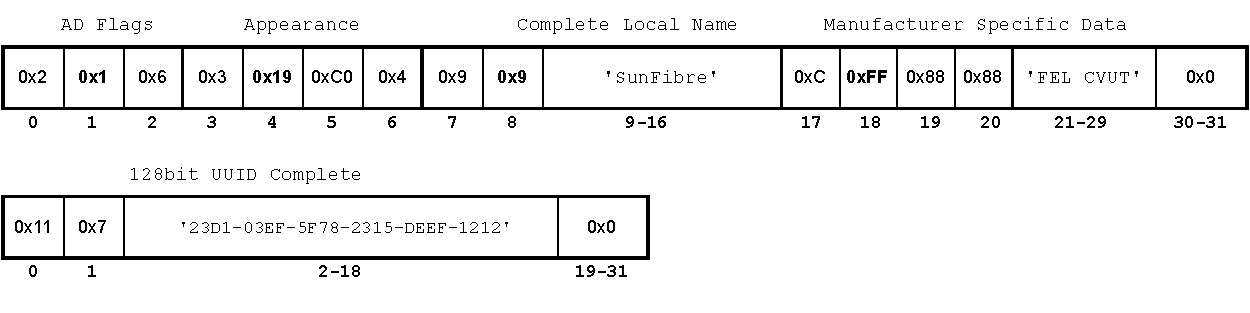
\includegraphics[ width=\textwidth]{SW_Firmware/Figs/app_ble_adpacket.pdf}
                \caption {Advertising and Scan Response Packet of light control unit}
                \label{figure:ad_packets}
            \end{figure}  
            
            The AD elements types and their values configured in the application are shown in table \ref{table:ad_elements}, the structure of the packets is in figure \ref{figure:ad_packets}.\\
            The advertising indication packet contains the flags AD element determining the discoverability and Bluetooth technology used, the appearance element defining the external appearance of the device, the advertised name and manufacturer data.\\
            The scan response packet further includes UUID of either Light Control Service or Maintenance Service (see section \ref{sec:app_ble_services}).
            
            
            \begin{table}[!ht]
                \begin{tabular}{l!{\vrule width 1pt}c}
                    \textbf{AD Type} &  \textbf{Value}\\ 
                    \Xhline{1\arrayrulewidth}
                    AD Flags \textbf{0x1} & 0x6 - \sss{General Disc. Mode, BR/EDR Not Sup.}\\
                    Appearance \textbf{0x19} & 0xC004 - \sss{Generic Control Device} \\
                    Complete Local Name \textbf{0x9} & SunFibre\\
                    Manufacturer Data \textbf{0xFF} & id: 0x8888, name: 'FEL CVUT'\\
                    128bit UUID Complete \textbf{0x7} & 23D1-03EF-5F78-2315-DEEF-1212\\
                \end{tabular}
                \caption{AD elements of the light control unit}
                \label{table:ad_elements}
            \end{table}
            
            % https://docs.silabs.com/bluetooth/latest/general/adv-and-scanning/bluetooth-adv-data-basic
            % https://btprodspecificationrefs.blob.core.windows.net/assigned-numbers/Assigned%20Number%20Types/Generic%20Access%20Profile.pdf
            
            % https://specificationrefs.bluetooth.com/assigned-values/Appearance%20Values.pdf
            % https://jimmywongiot.com/2019/08/13/advertising-payload-format-on-ble/
       
        \subsubsection{Advertising Modes}
            In order to optimize the battery consumption, two different advertising modes were configured (fast and slow).  The fast advertising runs for first three seconds after the advertising is turned on. In this mode, the advertising packets are broadcasted in short intervals to scan the peripheral quickly. If no device connects, a slow advertising mode is turned on when the packets are transmitted in longer intervals to save the battery.(see table with parameters \ref{table:ble_parameters}).
            
            The device stays advertising until a connection occurs or until a time interval determined by the current application state elapses (see the section about application timer - \ref{sec:apptimer}). 
            
        \subsubsection{Scanning Mode} 
            The scan interval and scan window parameters define how often and for how long a scanner listens for potential advertising packets \cite[20]{ble_book}.
            
            The floating button listens for advertising packets in 2500 ms intervals with an active scanning window of 1250 ms, meaning the radio is turned on 50 \% of the scanning time. 
            Hence, the worst case latency of successfully scanning the light control unit in a slow advertising mode is 2000 ms.
            
            The scanned advertising packets are filtered according to the device name. Once the peripheral is connected or when the application timer fires, the scanning is stopped.
            
    \subsection{Connection Parameters}
        \label{sec:app_connection_parameters}
        The connection parameters for a BLE connection are a set of properties of the link that determine how and how often the central and peripheral communicate. These parameters are a key factor in balancing throughput and power consumption. The parameters are exchanged when the connection is initially established, and they are always determined by the central. However, the peripheral can send a \verb|Connection Parameter Update Request| for changing them.\\
        \textbf{Connection Interval} is the time between the beginning of two consecutive connection events.\\
        \textbf{Slave Latency} is the number of events that a slave can skip if he doesn't have data to send without risking disconnection.\\
        \textbf{Connection Supervision Timeout} is the maximum time between two received data packets before a connection is considered as lost \cite[22--23]{ble_book}.
        

        The initial connection parameters are configured by central (floating button or smartphone). They allow greater throughput so that the data can be exchanged quickly at the start (initial reading of characteristics, writing to CCCD descriptors etc.).\\
        After five seconds from the connection establishment, the light control unit sends a \verb|Connection Parameter Update Request| demanding a greater connection interval. The connection interval value was set up to reduce battery consumption and get a reasonable latency, especially when the light mode is changed.
        
        All connection parameters are shown in table \ref{table:ble_parameters}. The slave latency is set to zero because the read or write commands initiated by central prevails.
        
        \subsection{Throughput Parameters}
            \textbf{MTU Size} is the maximum transmission unit of ATT protocol - payload size of ATT packets.\\
            \textbf{Data Length} is the size of usable payload of data packets.\\
            \textbf{Event Length} gives the maximum length of connection intervals. 
            
            Due to the fact that the data length of all BLE characteristics does not exceed 4 bytes (see section \ref{sec:app_ble_services}) and very few packet exchanges are needed, all throughput parameters were set to the lowest possible values to save the battery.

    \begin{table}[!ht]
        \begin{tabular}{l|c}
            \textbf{Type} & \textbf{Value} \\ 
            \Xhline{1\arrayrulewidth}
            Fast Advertising Interval & 100 ms\\
            Fast Advertising Duration & 100 ms\\
            Slow Advertising Interval & 1000 ms\\
            Slow Advertising Duration & x \\
            Scanning Interval & 2500 ms \\
            Scanning Active Window & 1250 ms \\
            Scanning Duration & x \\
            Initial Connection Interval & 200 ms\\
            Connection Interval & 1000 ms\\
            Connection Slave Latency & 0 \\
            Connection Supervision Timeout & 4000 ms\\
            MTU Size & 23\\
            Data Length & 27\\
            Event Length & 7.5 ms\\
        \end{tabular}
        \caption{Selected BLE parameters}
        \label{table:ble_parameters}
    \end{table}
        
    \subsection{Security}
        \label{sec:app_ble_security}
        A connection can operate in a particular security mode. GAP defines two security modes with several levels per mode.\\
        \textbf{Security Mode 1} enforces security by means of encryption containing 3 levels. Level 1 - no security, level 2 - unauthenticated encryption, level 3 - authenticated encryption.\\
        \textbf{Security Mode 2} enforces security through data signing, and it has two levels. Level 1 - unauthenticated data signing, level 2 - authenticated data signing. \cite[45--47]{ble_book}
            
        Because both the light control unit and floating button are keyboardless and screenless devices, displaying a passkey is not possible, so the only possible key generation and exchange method is \textbf{Just Works}. Hence, security mode 1, level 2 (encryption required, authentication and authorization not required) is necessary for communication and data exchanges. This security level doesn't provide any protection against MITM (Man In The Middle) attacks.
    
    \subsection{BLE Services}
        \label{sec:app_ble_services}
        Two custom primary services with 128-bit UUID were implemented to provide data - \textit{Light Control Service} and \textit{Maintenance Service}. The light control unit uses both of them, floating button only the latter one when in peripheral mode.\\
        Additionally, \textit{Secure DFU Service} service was added to both devices. It is also a primary service with 128-bit UUID implemented by Nordic. 
        
        \begin{figure} [!ht]
    	    \centering
    	    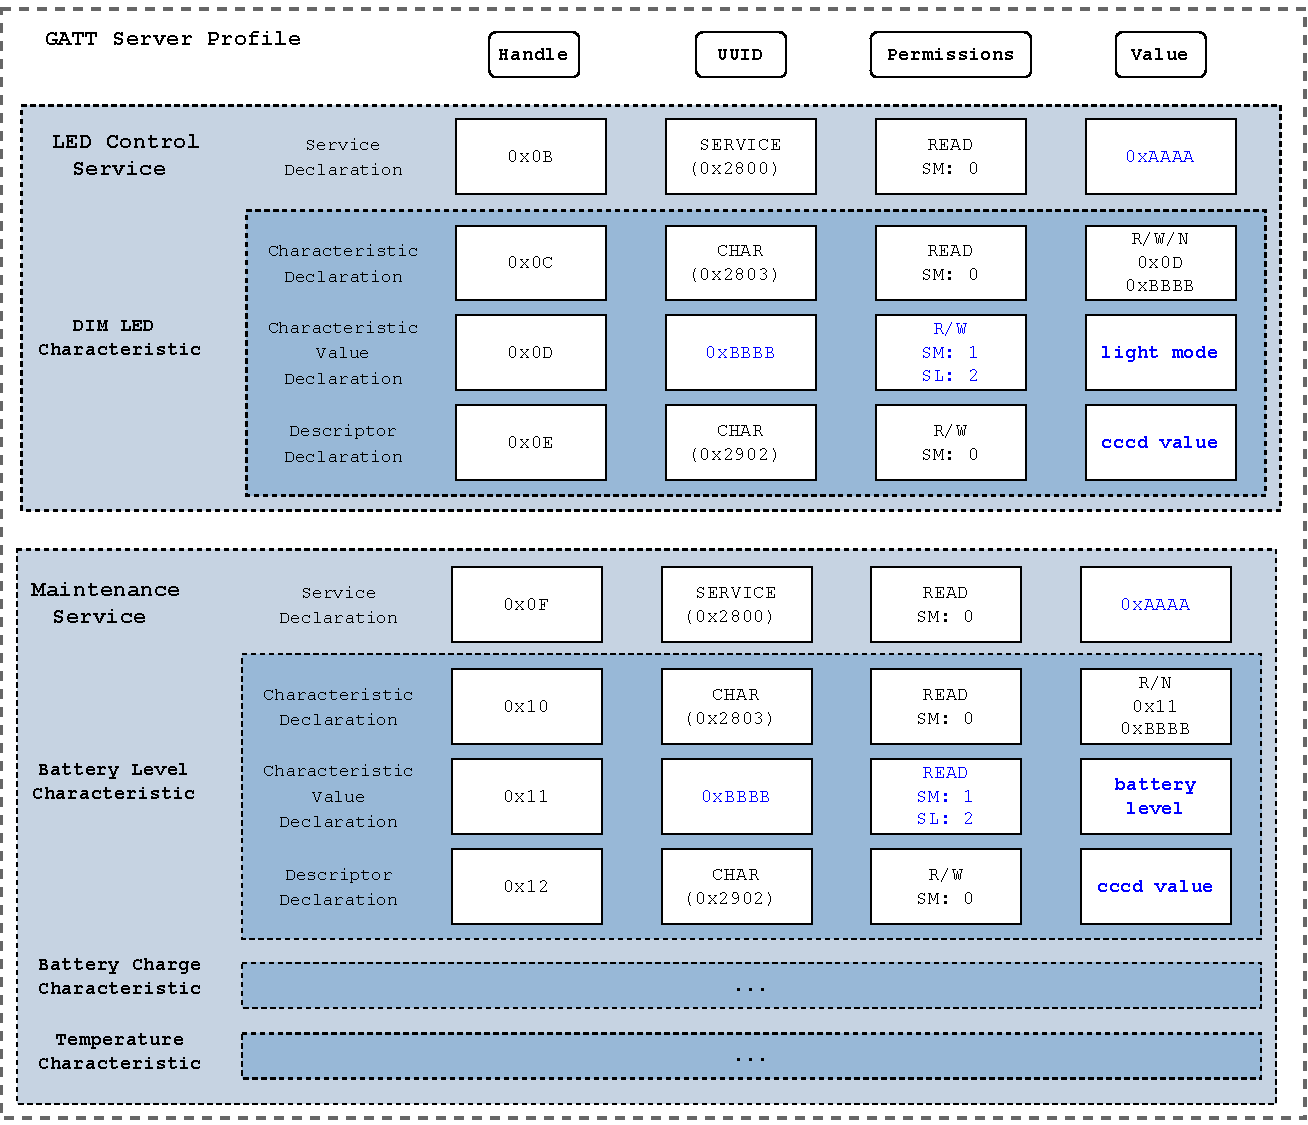
\includegraphics[ width=\textwidth]{SW_Firmware/Figs/app_ble_gatt.pdf}
            \caption {GATT model of the light control unit}
            \label{figure:gatt_model}
        \end{figure}  
        
        \subsubsection{LED Control Service}
            Base UUID: \textbf{1212-efde-1523-785fef13d123}
            
            The LED Control Service serves as a controller allowing changing the light modes (see section \ref{sec:urs_lcu}). It contains only one characteristic.
            
            \textbf{Light Mode Characteristic}\\
            % LENGTH %
            The characteristic value is a one-byte long integer that represents the current light mode. The value corresponds with the light modes defined in section \ref{sec:light_modes}.\\
            % VALUE UPDATES 
            A light mode can be either incremented by writing -1 to the characteristic or changed directly by writing the light mode number directly. The characteristic value is also updated after every light mode change that does not come from BLE - button press or RFID detection.\\
            In case of a light mode change, a notification is sent to all connected clients if enabled previously.
            % PROPERTIES PERMISSIONS 
            The characteristic properties are read/write/notify. The link must be encrypted to read or write - security mode 1, security level 2 (see section \ref{sec:app_ble_security} explaining the security modes).
            
            
        \subsubsection{Maintenance Service}
            Base UUID: \textbf{1413-f0df-1624-7960f014d224}
            
            The Maintenance Service exposes supporting (maintenance) data to a client. It includes these three characteristics:
            \begin{itemize}
            \setlength\itemsep{0.2em} 
                \item \textbf{Battery Charging Characteristic},
                \item \textbf{Battery Level Characteristic},
                \item \textbf{Temperature Characteristic}.
            \end{itemize}
            
            % LENGTH %
            The Battery Charging and Battery Level characteristic values are one-byte long and represent the estimated battery level and charging status.
            The Temperature characteristic value is a four-byte long characteristic and reflects the board's temperature in Celsius degrees.\\
            % VALUE UPDATES 
            All three characteristic values can only be read. Section \ref{sec:battery_estimation} explains how and how often they are updated.
            A notification for a particular characteristic is sent to each connected client only if its value changes and when notifications are enabled.
            % PROPERTIES PERMISSIONS 
            The characteristic properties are read/notify. The security requirements to obtain data are the same as for Light Mode Characteristic.
            
        \subsubsection{Secure DFU Service}
        
            Base UUID: \textbf{f315-4f60-9fB8-838830daea50}
            The main purpose of the Secure DFU Service is a remote (buttonless) activation of the DFU mode. 
            
            \textbf{Buttonless DFU Characteristic}\\
            When the client writes to this characteristic, a unique value is written to the \sss{GPREGRET} register, and a system reset to DFU mode is executed (see section \ref{sec:buttonless_activation} which comments the DFU activation process).
            % PROPERTIES PERMISSIONS 
            The characteristic properties are write/indicate. Neither the encryption of the link nor the authorization is required - security mode 1, security level 1 (see section \ref{sec:app_ble_security} explaining the security modes).
        
        \subsubsection{Service and Characteristic Discovery}
            To read or write a characteristic value or a descriptor, the central must know its attribute handles.\\ 
            However, because the handles are assigned to the attributes by SoftDevice and might have arbitrary values, the service and characteristics discovery is necessary. The central performs discovery of primary services at first, followed by discovery of all characteristics of a particular service. The characteristic value attribute handles are read from characteristic declarations (see the model of GATT server in figure \ref{figure:gatt_model}).\\
            Since the attribute handles are consistent, if the layout of the GATT server model does not change, they are cached and stored in flash so that during the next connection, the discovery procedure is not needed.
            
            Nordic libraries were used for discovery procedures and attribute handles caching on the floating button.


          
\section{Common Business Logic}
    \label{sec:app_businnes_logic}
    A general explanation of system devices' roles and communication between them is described in this section. If further introduces common terms used in the application logic.
    
    The light control unit, a BLE peripheral, can be connected to multiple centrals (floating button or smartphone/smartwatch applications). To connect a new central, the bonding procedure must be carried out first. The bonding is required only during the first connection. Then it can be skipped (searching procedure) - see section \ref{sec:bonding} with a more detailed description of these procedures.\\
    When a central is connected to the light control unit, it can read its BLE characteristics (light mode, battery level, charging status or temperature) or write to them - change the light mode or enter the DFU mode. Notifications synchronise these characteristic values with centrals. So, for example, if the light mode is changed by RFID, its new value is sent to all connected centrals.\\
    
    The floating button can operate as both BLE central and BLE peripheral simultaneously. Changing the light modes on the light control unit is possible in the central role. The peripheral mode enables reading maintenance information of the floating button (battery level, charging status, temperature) through a smartphone application.
    
    \subsection{Application States}
        \label{sec:app_states}
        The application states prescribe the system's behaviour (whether the advertising/scanning is turned on, the whitelist is used or when the application timer fires etc.). The system actions (procedures) are triggered by application events (section \ref{sec:app_events}) and are dependent on the current application state.\\
        The application states differ for light control unit (\ref{sec:lcu_app_states}) and floating button (\ref{sec:fb_app_states}).
        
    \subsection{Application Events}
        \label{sec:app_events}
        The application events are generated by various system parts such as BLE, battery, buttons, RFID or application timer. They are handled in an application handler based on the type of the event and the current application state.\\
        Some events require additional context - further specification of the event, for example, which connection was disconnected.\\
        The table \ref{table:app_events} shows the list of all application events. Their meaning should be self-explanatory, and their names correspond to the labels of dashed lines in the state diagrams (figures \ref{figure:state_diagram_wakeup} - \ref{figure:state_diagram_bonding}).
        
        \begin{table}[!ht]
            \begin{tabular}{l!{\vrule width 1pt}c}
                \textbf{Application Event} &  \textbf{Source}\\ 
                \Xhline{1\arrayrulewidth}
                \sss{EVT\_BTN\_SHORT\_CLICK} & button \\\hline
                \sss{EVT\_BTN\_MEDIUM\_CLICK} & button \\\hline
                \sss{EVT\_BTN\_LONG\_CLICK} & button \\\hline
                \sss{EVT\_BTN\_VERY\_LONG\_CLICK} & button \\\hline
                \sss{EVT\_BTN\_PRESS\_START} & button \\\hline
                \sss{EVT\_BTN\_PRESS\_INTERVALPASSED} & button \\\hline
                \sss{EVT\_BLE\_CONNECTED} & BLE\\\hline
                \sss{EVT\_BLE\_CONNECTED\_AND\_BONDED} & BLE\\\hline
                \sss{EVT\_BLE\_DISCONNECTED} & BLE\\\hline
                \sss{EVT\_BLE\_DISCONNECTED} & BLE\\\hline
                \sss{EVT\_BLE\_SECURITY\_START} & BLE\\\hline
                \sss{EVT\_BLE\_SECURITY\_ERROR} & BLE\\\hline
                \sss{EVT\_BLE\_BONDS\_REMOVED} & BLE\\\hline
                \sss{EVT\_BATTERY\_CHARGER\_CONNECTED} & battery \\\hline
                \sss{EVT\_BATTERY\_CHARGER\_DISCONNECTED} & battery\\\hline
                \sss{EVT\_BATTERY\_MEASURED} & battery\\\hline
                \sss{EVT\_RFID\_DETECTED} & RFID\\\hline
                \sss{EVT\_TIMER} & RTC
            \end{tabular}
            \caption{A list of supported application events}
            \label{table:app_events}
        \end{table}
        
    \subsection{Application Timer}
        \label{sec:apptimer}
        The application timer is based on RTC. As long as it elapses, an interrupt is triggered, application event \sss{EVT\_TIMER} is generated and the application enters a new state. 
        Depending on the new state, the value of the timer is set (see table \ref{table:lcu_app_states} or \ref{table:fb_app_states} below for application timer values).\\
        In order to prevent the timer from firing during long clicks, a detection of a button press (application event \sss{EVT\_BTN\_PRESS\_START}) immediately resets/extends the current timer regardless of the current state.
        
        The timer values - intervals in seconds for which the application stays in a particular state are specified in a user configuration file in \verb|app_config.h| (see section \ref{sec:configuration_files}).
            
        
        

\section{Light Control Unit}
    This section provides a specification of BLE properties, user interface and the business logic related to the light control unit. It serves as a detailed description. The general description with functional requirements is provided further in section \ref{sec:urs_lcu}. 
    
    \subsection{BLE Properties}
        \label{sec:lcu_ble_parameters}
        According to GAP, the light control unit behaves as a scannable and connectable peripheral (slave). In particular application states (see \ref{sec:lcu_app_states}), it advertises with the name \textbf{SunFibre} and accepts incoming connections from a central - smartphone or floating button.\\
        When the connection is established, the unit follows the central's timings (connection interval) but requests an update of connection parameters after a few seconds.\\
        The data are read or written regularly through BLE services - \textit{LED Control}, \textit{Maintenance} or \textit{Secure DFU}. Up to 5 centrals could be connected at the same time.
        
        More information on advertising, connection parameters and BLE services can be found in section \ref{sec:app_ble}. The structure of advertising packet is in figure \ref{figure:ad_packets} and the GATT layout in figure \ref{figure:gatt_model}.
        
        
    \subsection{User Interface} 
        One push-button and three RGB LEDs on the light control unit board were used to design a user interface.
        
        \textbf{Button}\\
            Pressing the button generates button application events (see \ref{sec:app_events}). A short, medium, long and very long clicks are distinguished (see the section \ref{sec:fw_buttons} commenting buttons and table \ref{table:btn_click} with click's durations).\\
            To put it simply, a short button click changes the light mode, a medium-long click makes the device to be visible for known (already bonded) centrals, a long click starts a bonding procedure (searching for new devices), and a very long click resets the device.
        
        
        \textbf{RGB LEDs}\\
            \label{sec:lcu_rgb_leds}
            The first LED is called \textit{state LED} and its color and blinking determine the application state (see section \ref{sec:app_states}). If the LED is blinking, the device is advertising.\\
            The second one, \textit{battery LED}, indicates the level of battery (see the colors corresponding to battery levels in table \ref{table:battery_levels}. If the LED is blinking, the battery is being charged.\\
            The third, \textit{helper LED}, blinks if an interval for recognizing a particularly long click passed (application event \sss{EVT\_BTN\_PRESS\_INTERVALPASSED}. As a result, the number of blinks helps the user know when to release the button for a particular long click.
            
            
            The colors of LEDs corresponding to application states and the button click intervals are configured in \verb|app_config.h|.
            
    
    \subsection{Business Logic}
        This subsection introduces the application logic of the light control unit that has been designed and implemented according to customer requirements. The functionality is split into multiple so-called procedures, each one further explained by a state diagram.
                
        \subsubsection{Application States}
            \label{sec:lcu_app_states}
            The application states on the light control unit are distinguished by color of \textit{state LED}. If the device is advertising, the LED is blinking. Immediately after a connection, the blinking is stopped. 
            
            The table \ref{table:lcu_app_states} briefly explains the behaviour in application states and shows their corresponding LED color and application timer interval. \textit{C} denotes the number of previously connected centrals, \textit{B.} means blinking.
            
            \begin{table}[!h]
                \catcode`\-=12
                \resizebox{\columnwidth}{!}{%
                    \begin{tabular}{l!{\vrule width 1pt}ccr}
                        \textbf{Application State} &  \textbf{Description} &  \textbf{Timer} & \textbf{LED}\\ 
                        \Xhline{1\arrayrulewidth}
                        \sss{SYSTEM OFF} & deep sleep & $\infty$ & off \\
                        \hline
                        \sss{IDLE} & sleep, action waiting & 20 s &  off \\
                        \hline
                        \sss{NOT CONNECTED} & $C = 0$, action waiting & 20 s &\tikzsymbol{fill=red}\\
                        \hline
                        \sss{CONNECTED}  & $C > 0$, action waiting & $\infty$ & \tikzsymbol{fill=green} \\
                        \hline
                        \multirow{2}{*}{\sss{SEARCHING ADVERTISING}}  & $C = 0$, connection waiting, whitelist & 40 s & B. \tikzsymbol{fill=yellow}\\
                        \cline{2-4}
                        & $C > 0$, connection waiting,  whitelist & 15 s & B. \tikzsymbol{fill=green} \\
                        \hline
                        \multirow{2}{*}{\sss{SEARCHING CONNECTED}} & $C = 0$, security request waiting & 10 s & \tikzsymbol{fill=yellow} \\
                        \cline{2-4}
                        & $C > 0$, security request waiting & 10 s & \tikzsymbol{fill=green} \\
                        \hline
                        \sss{BONDING ADVERTISING} & connection waiting, no whitelist  & 15 s & B. \tikzsymbol{fill=blue}\\
                        \hline
                        \sss{BONDING CONNECTED}  & pairing request waiting &  10 s & \tikzsymbol{fill=blue}\\\hline
                    \end{tabular}
                }
                \caption{Application states of light control unit}
                \label{table:lcu_app_states}
            \end{table}
           
        \subsubsection{Wakeup Procedure}
            \label{sec:wakeup}
            
        \textbf{\sss{IDLE}} is the default state that the application enters after reboot. To proceed to the searching procedure, the user must click on the button (medium-long). In case that there are no previously bonded peers saved in flash, the device moves to \textbf{\sss{NOT CONNECTED}} state, turning the \textit{state LED} red and allowing further only bonding procedure.
           
            \begin{figure} [!hb]
        	    \centering
        	    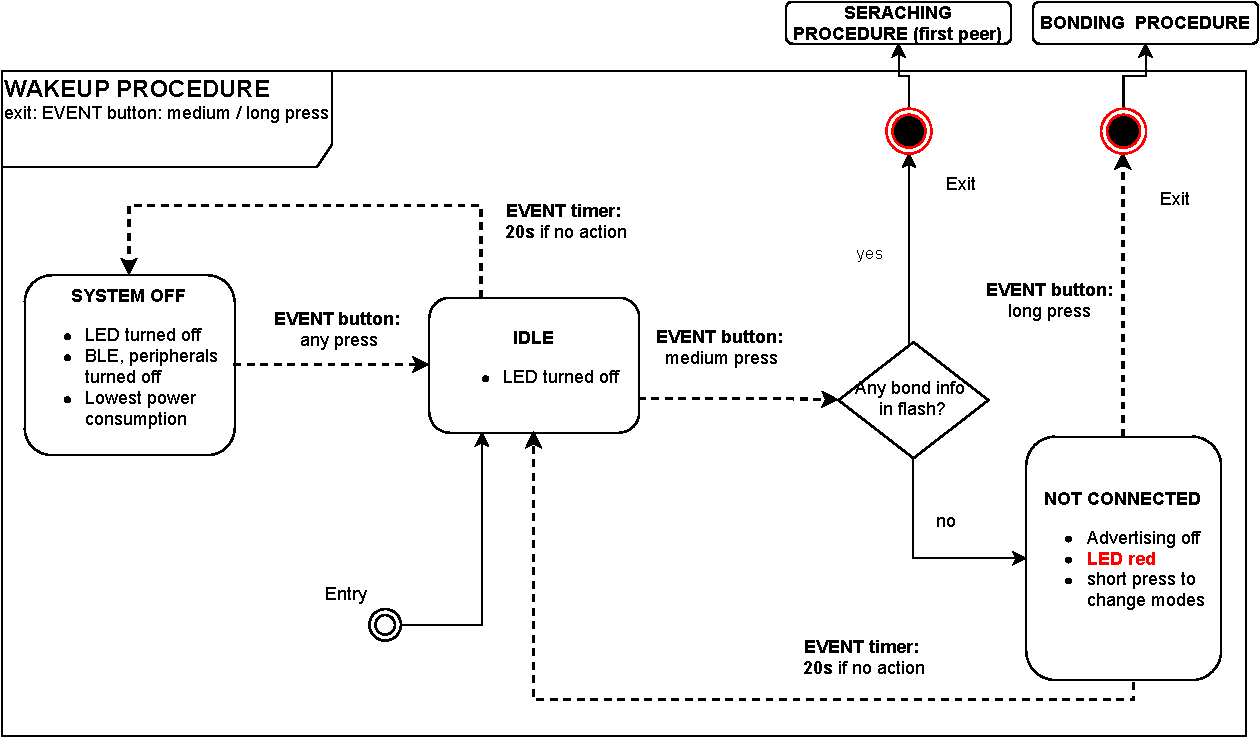
\includegraphics[ width =\textwidth]{SW_Firmware/Figs/wakeup_procedure.pdf}
                \caption {State diagram - application start (wakeup)}
                \label{figure:state_diagram_wakeup}
            \end{figure}  
            
            \textbf{Deep Sleep}\\
            If the battery level is under a critical level (see the section \ref{sec:battery_estimation}) or when the inactivity timer elapses in \sss{IDLE} state, the unit enters \textbf{\sss{SYSTEM OFF}} mode. In order to reduce the battery usage to the minimum, all peripherals besides GPIO are turned off and the device could wake up only by an arbitrary long button click.
            
        \subsubsection{Connected Procedure}
            \label{sec:connection}
            When in \textbf{\sss{CONNECTED}} state, the device is connected to at least one central and does not advertise. It allows R/W operations of BLE characteristics (see section \ref{sec:app_ble_services}).\\ 
            By a long button click, the user can start the bonding procedure with a new central, a medium-long button click allows searching for bonded centrals.\\
            If all connected devices disconnect, the \sss{SEARCHING ADVERTISING} state is entered automatically and the searching procedure is started. 
            
            \begin{figure} [!ht]
        	    \centering
        	    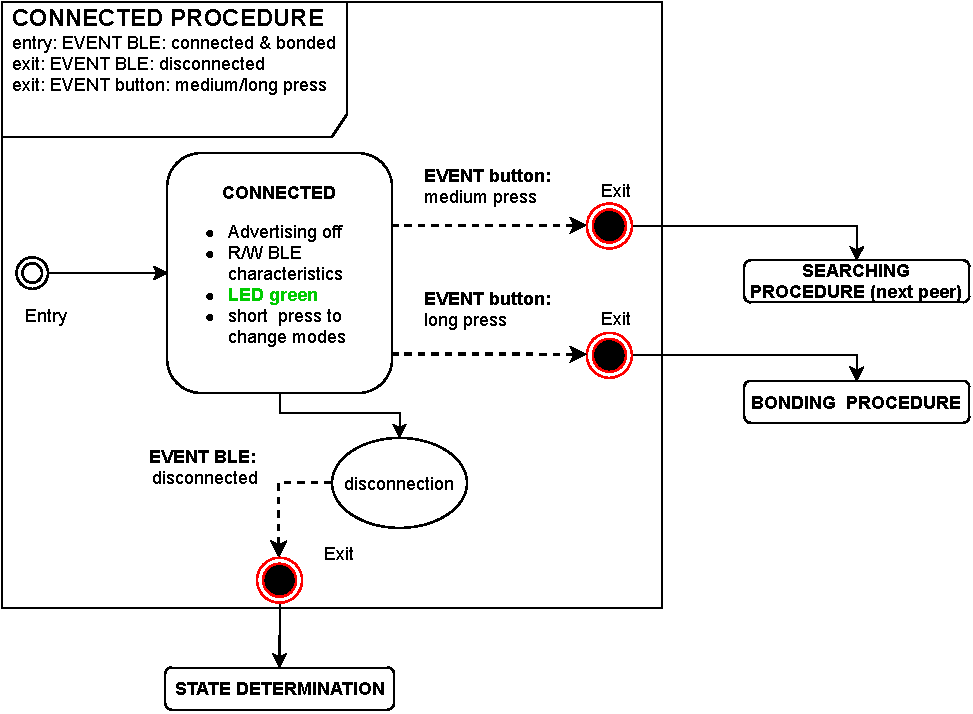
\includegraphics[ width =0.9\textwidth]{SW_Firmware/Figs/connected_procedure.pdf}
                \caption {State diagram - connected state}
                \label{figure:state_diagram_connected}
            \end{figure}  
        
        \subsubsection{Searching Procedure}
            \label{sec:searching}
            The searching procedure can be started by a medium-long click from states: \sss{IDLE} or \sss{CONNECTED}.
            While in \textbf{\sss{SEARCHING ADVERTISING}} state, only previously bonded devices are allowed to connect (the device advertise with a whitelist). Thus all connection requests from unknown centrals are rejected.
            The \textit{state LED} is blinking, and its color is either yellow (if no centrals are connected) or green (at least one another central is connected).\\ 
            If a connection from a known central occurs, advertising is stopped and LED stops blinking - \textbf{\sss{SEARCHING CONNECTED}}. The device waits until the connected central starts the GAP encryption procedure (encryption of the link with the previously negotiated LTK security key). Providing that the security is successful (LTKs on both sides are valid), the \sss{CONNECTED} state is entered. Otherwise, an error is signalized .
            
            \begin{figure} [!ht]
        	    \centering
        	    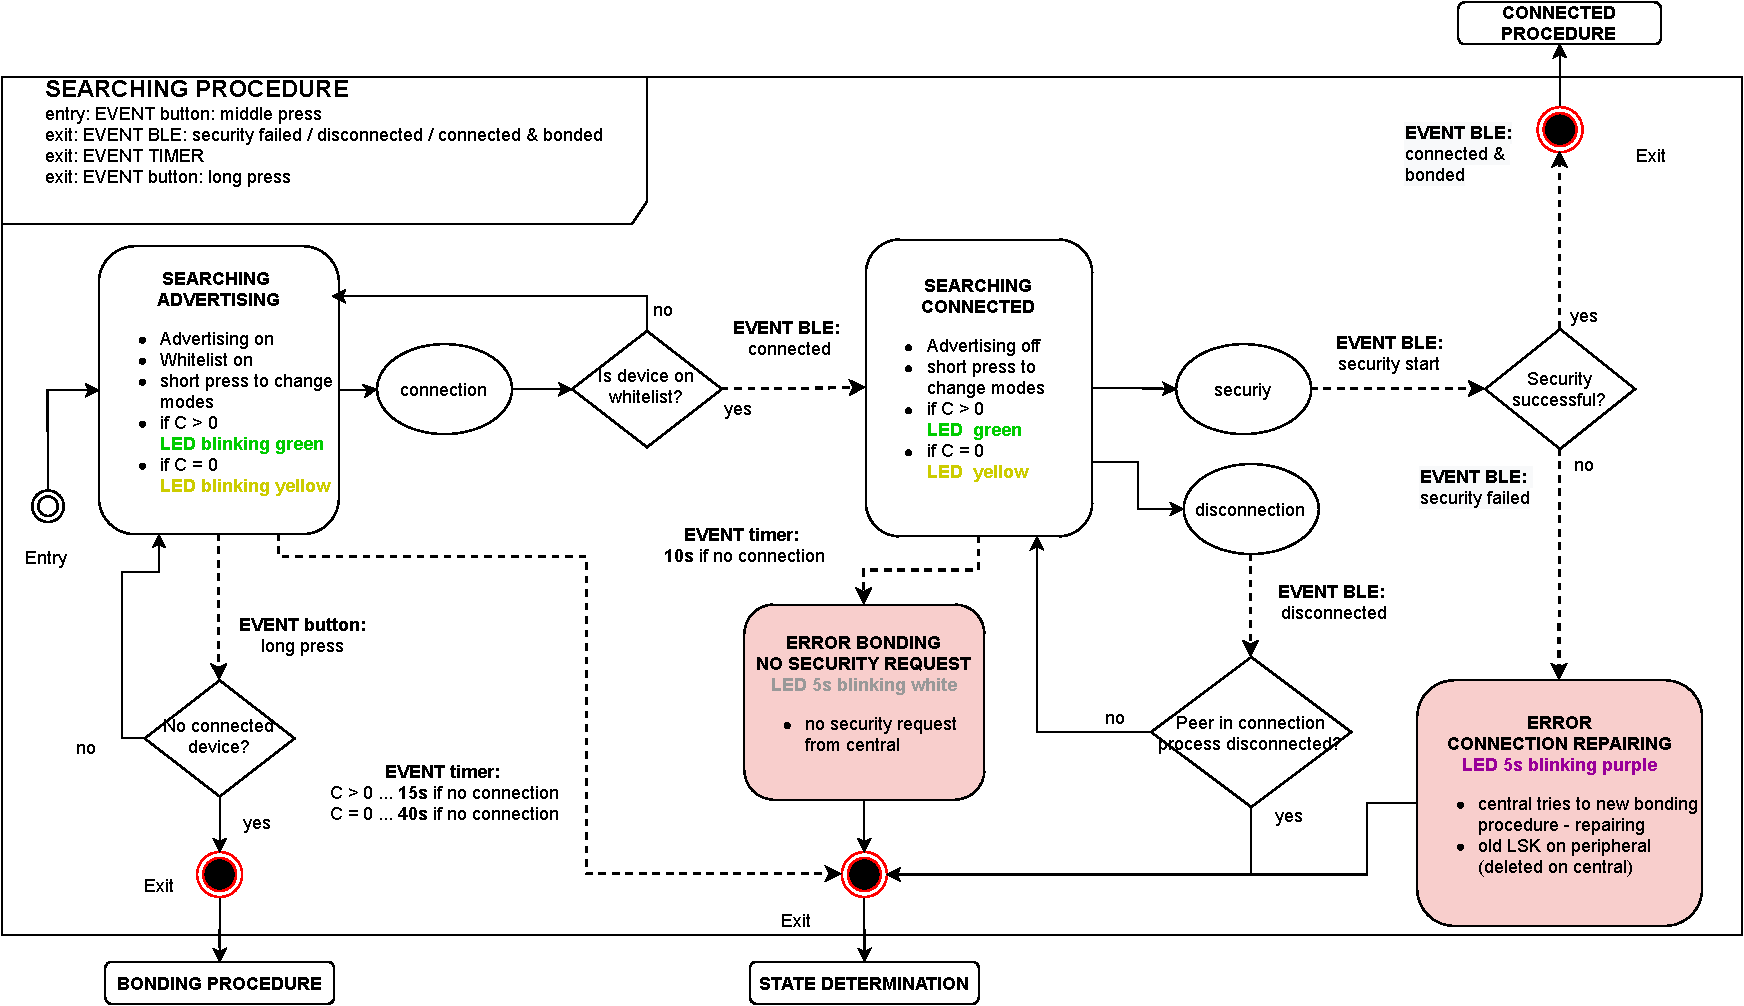
\includegraphics[ width =1.1\textwidth]{SW_Firmware/Figs/searching_procedure.pdf}
                \caption {State diagram - searching for device}
                \label{figure:state_diagram_searching}
            \end{figure}  
            
            \begin{figure} [!ht]
        	    \centering
        	    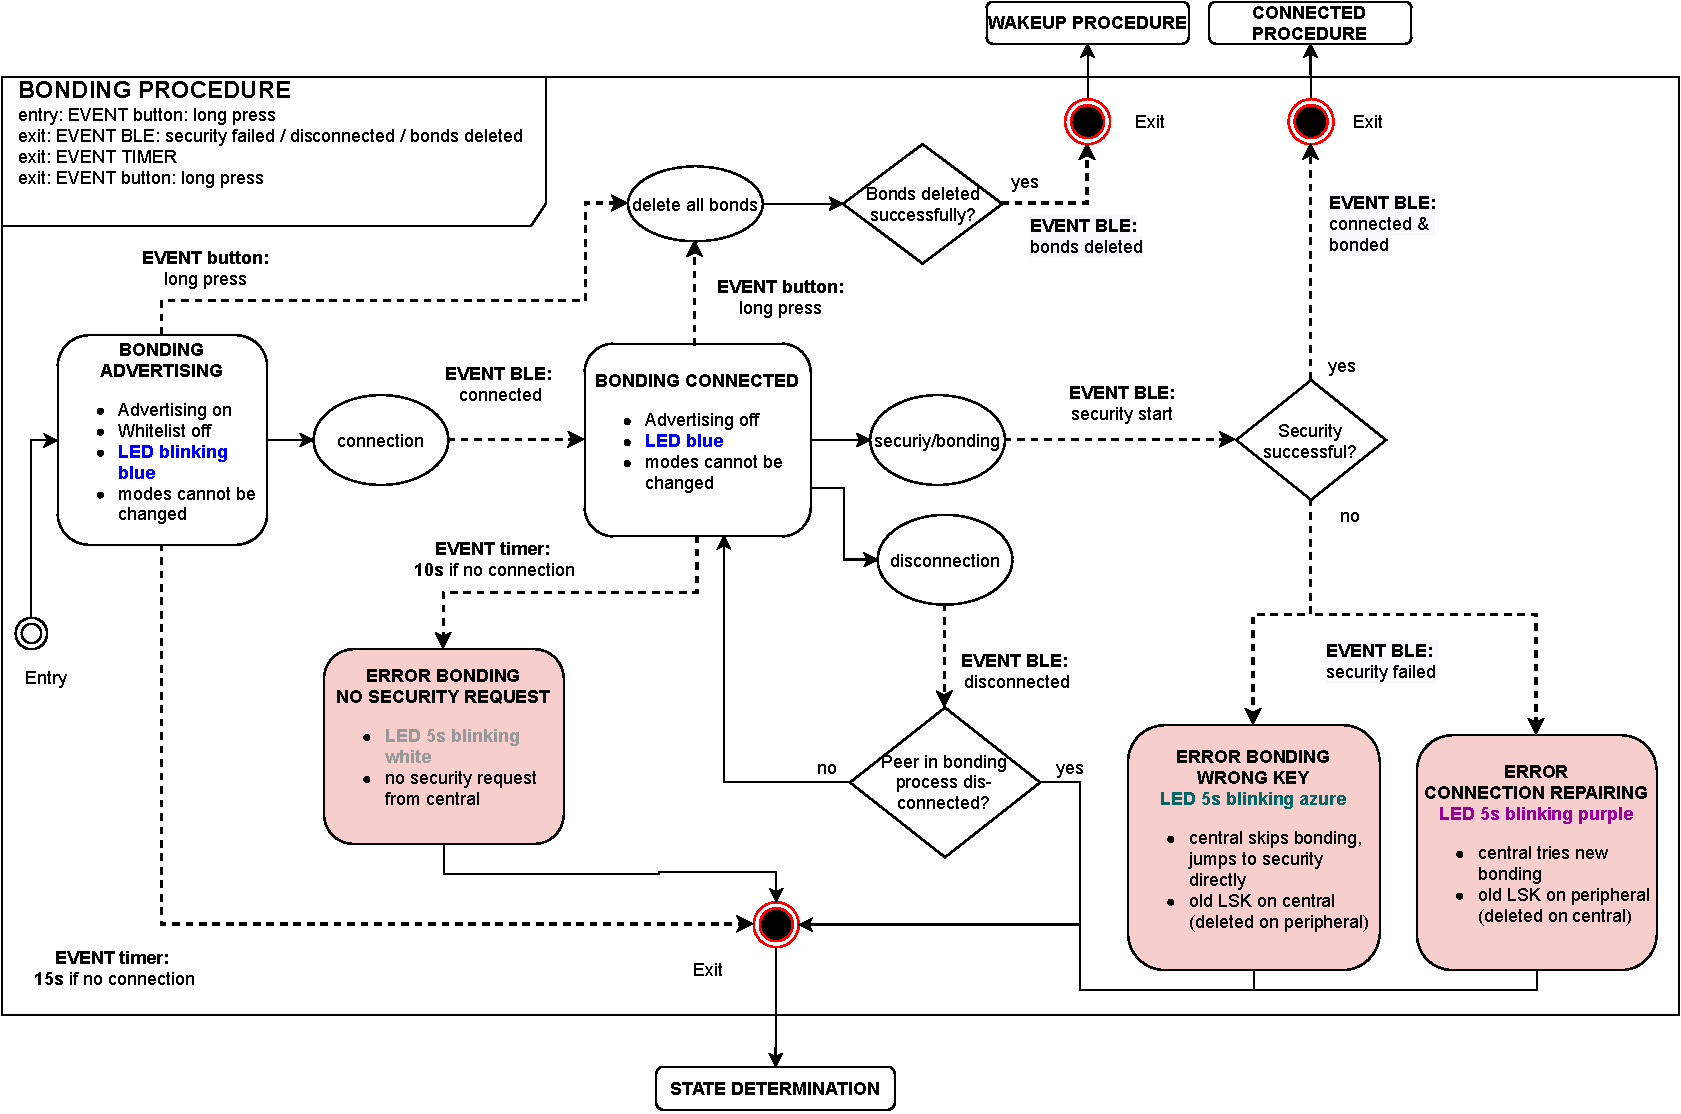
\includegraphics[ width =1.1\textwidth]{SW_Firmware/Figs/bonding_procedure.pdf}
                \caption {State diagram - bonding with a new device}
                \label{figure:state_diagram_bonding}
            \end{figure}  
            
        \subsubsection{Bonding Procedure}
            \label{sec:bonding}
            The bonding procedure is entered by a long button click from any of the states: \sss{NOT} \sss{CONNECTED}, \sss{SEARCHING} \sss{ADVERTISING} or \sss{CONNECTED}.
            During \textbf{\sss{BONDING}} \textbf{\sss{ADVERTISING}} state, all connection requests are accepted (the device advertises without a whitelist).\\
            In case of a new connection, the advertising is stopped, and the \textit{state LED} stops blinking - \textbf{\sss{BONDING CONNECTED}}. The device waits until the central initiates the GAP authentication procedure (pairing and bonding - exchange of security keys). The \sss{CONNECTED} state is then entered if the authentication procedure is successful. Otherwise, an error is indicated (further described in \ref{sec:error_states}).
            
            \newpage 
            
            \textbf{Deleting Bonds}\\
            The user can delete all stored bonding security long term keys (LTKs) from flash. This action requires two long button click. Upon the removal, the device enters \sss{NOT} \sss{CONNECTED} state. 
            
        \definecolor{azure}{rgb}{0.0, 1.0, 1.0} 
        \definecolor{purple}{rgb}{1.0, 0.0, 1.0} 
        
        \subsubsection{Error States}
            \label{sec:error_states}
            Bonding or searching procedures might fail for several reasons. The most important ones are indicated to the user by a few LED blinks and are shown in the table \ref{table:error_states}. The color of \textit{state LED} determines the type of the error.
            
            \noindent\textbf{\sss{NO SECURITY REQUEST}} refers to a situation when a central connects to the peripheral but does start the encryption or authentication procedure so that the application timer elapses.\\
            \textbf{\sss{MISSING KEY}} error might occur if central tries to encrypt the connection by using a LTK that is not present or valid on the peripheral. This error is usually caused by deleting bonding information on the peripheral but not on the central.\\
            \textbf{\sss{REPAIRING}} appears when a central initiates the authentication procedure (pairing), and generates a new STK despite being previously bonded (the old LTK is still stored on the peripheral). This error is usually caused by the deletion of bonding information on the central but not on the peripheral.\\
            Nevertheless, this error might be prevented when repairing is explicitly allowed. Then the central can always bond with the light control unit regardless of previously saved LTK.
            
            
            \begin{table}[H]
                \resizebox{\columnwidth}{!}{%
                    \begin{tabular}{l!{\vrule width 1pt}cr}
                        \textbf{Error} &  \textbf{Reason} & \textbf{LED}\\ 
                        \Xhline{1\arrayrulewidth}
                        \sss{NO SECURITY REQUEST} & no encryption/authentication procedure & \tikzsymbol{fill=white} \\\hline
                        \sss{MISSING KEY} & no LTK on peripheral, old LTK on central & \tikzsymbol{fill=azure} \\\hline
                        \sss{REPAIRING} & old LTK on peripheral, new LTK on central & \tikzsymbol{fill=purple} \\\hline
                    \end{tabular}
                }
                \caption{Error states of light control unit.}
                \label{table:error_states}
            \end{table}
            
\section{Floating Button}
    This section is devoted to the specification of BLE properties and the user interface of the floating button. It also gives a detailed description of the business logic. The general description with functional requirements of the floating button is provided in the section \ref{sec:urs_fb}. 

    \subsection{BLE Properties}
        \label{sec:fb_ble_parameters}
        In comparison with the light control unit, the floating button can operate as both central and peripheral.\\
        In the central (master) mode, it behaves as an active scanner, listening for advertising packets and initiating a connection with the first found light control unit. It determines the initial connection parameters and performs a discovery procedure of BLE characteristics. When the connection is established and discovery completed, it can write or read to \textit{Light Control Service} characteristics on the light control unit.\\
        At the same time, the unit could act as a scannable and connectable peripheral (slave), sending connectable advertising packets with its name \textbf{SunFibre-btn} and accepting incoming connections from a central - smartphone. The central then determines the connection intervals and can read characteristic values of \textit{Maintenance Service} or write to the \textit{Secure DFU Service}.\\
        Only one connection is possible in both modes (one central and one peripheral).
        
        More information on advertising, connection parameters and BLE services can be found in section \ref{sec:app_ble}.
    
    \subsection{User Interface}
        The floating button's user interface is based on two-push buttons and a 5x5 LED array.
        
        \textbf{Button}\\
            Clicking on the buttons generates application events (\ref{sec:app_events}). A short, medium, long and very long clicks are distinguished (see table \ref{table:btn_click}) in the same way as on the light control unit.\\
            The left button controls the central mode. A short click allows changing the light modes on the peripheral (only if connected), a medium-long click makes the device scan for peripherals, a long click disconnect device, and a very long click removes bonds.\\
            The peripheral mode is controlled by the second (right button). To put it simply, a medium click starts advertising, a long click allows disconnecting a connected device and a very long click resets the device.
            
        \textbf{LED Matrix}\\
            The LED matrix helps to determine the application state by showing a particular letter (see table \ref{table:fb_app_states}).   
            
        The LED matrix letters corresponding to application states and the button intervals are configured in \verb|app_config.h|.
        
        
    \subsection{Business Logic}
        In this subsection, the application logic of the floating button is introduced and its behaviour explained on state diagrams. 
        
        \subsubsection{Application States}
        \label{sec:fb_app_states}
            The floating button keeps two application states - one for central mode and one for peripheral mode. The application events generated by the left button influence the central state, the events from the right button the peripheral state. The BLE application events are handled based on the type of connection, whether they apply to central or peripheral mode.\\
            
            The application states are distinguished by the alphabet letters visualized by the LED matrix. Since the peripheral mode is less frequent and short-term, the peripheral state are prioritized. The central states (\sss{CENTRAL IDLE}, \sss{CENTRAL SCANNING}, \sss{CENTRAL CONNECTED}) are visualized only if the peripheral state is \sss{IDLE}. The letter \textbf{\large P} is used for all peripheral states, because the connection status could be immediately guessed from the smartphone application (the floating button can connect only to a smartphone in the peripheral mode).
            
            The table \ref{table:fb_app_states} briefly describes the behaviour in particular application states. It also shows the application timer intervals and LED matrix letters associated with the states.
        
            \begin{table}[!h]
                \resizebox{\columnwidth}{!}{%
                    \begin{tabular}{l!{\vrule width 1pt}ccr}
                        \textbf{Application State} &  \textbf{Description} &  \textbf{Timer} & \textbf{LED Matrix}\\ 
                        \Xhline{1\arrayrulewidth}
                        \sss{SYSTEM OFF} & deep sleep & $\infty$ & off \\\hline
                        \sss{CENTRAL IDLE} & action waiting & 20 s &  \large \textbf{I} \small iff \sss{P. IDLE} \normalsize  \\\hline
                        \sss{CENTRAL SCANNING} & scanning, connection waiting & 20 s & \large \textbf{S} \small iff \sss{P. IDLE} \normalsize\\\hline
                        \sss{CENTRAL CONNECTED}  & action waiting & $\infty$ & \large \textbf{C} \small iff \sss{P. IDLE} \normalsize\\\hline
                        \sss{CENTRAL ERROR}  & action waiting & $\infty$ & \large \textbf{E} \small iff \sss{P. IDLE} \normalsize\\\hline
                        \sss{PERIPHERAL IDLE} & action waiting & 20 s & x \\\hline
                        \sss{PERIPHERAL ADVERTISING} & advertising, connection waiting & 20 s & \large \textbf{P} \\\hline
                        \sss{PERIPHERAL CONN. ACCEPTED} & security request waiting & 10 s & \large \textbf{P} \\\hline
                        \sss{PERIPHERAL CONNECTED} & action waiting & $\infty$ & \large \textbf{P}\\\hline
                    \end{tabular}
                }
                \caption{Application states of the floating button.}
                \label{table:fb_app_states}
            \end{table}
        
        \subsubsection{Wakeup procedure}
            After the system reboot, the device enters central and peripheral \sss{IDLE} states waiting for action - starting scanning or advertising.
            
            \textbf{Deep Sleep}\\
            If the battery level is under a critical level (see section \ref{sec:battery_estimation}) or when both central and peripheral application timers elapse in \sss{IDLE} states, the unit enters \textbf{\sss{SYSTEM OFF}} state in the same way as on the light control unit.  
            
            \begin{figure} [!ht]
        	    \centering
        	    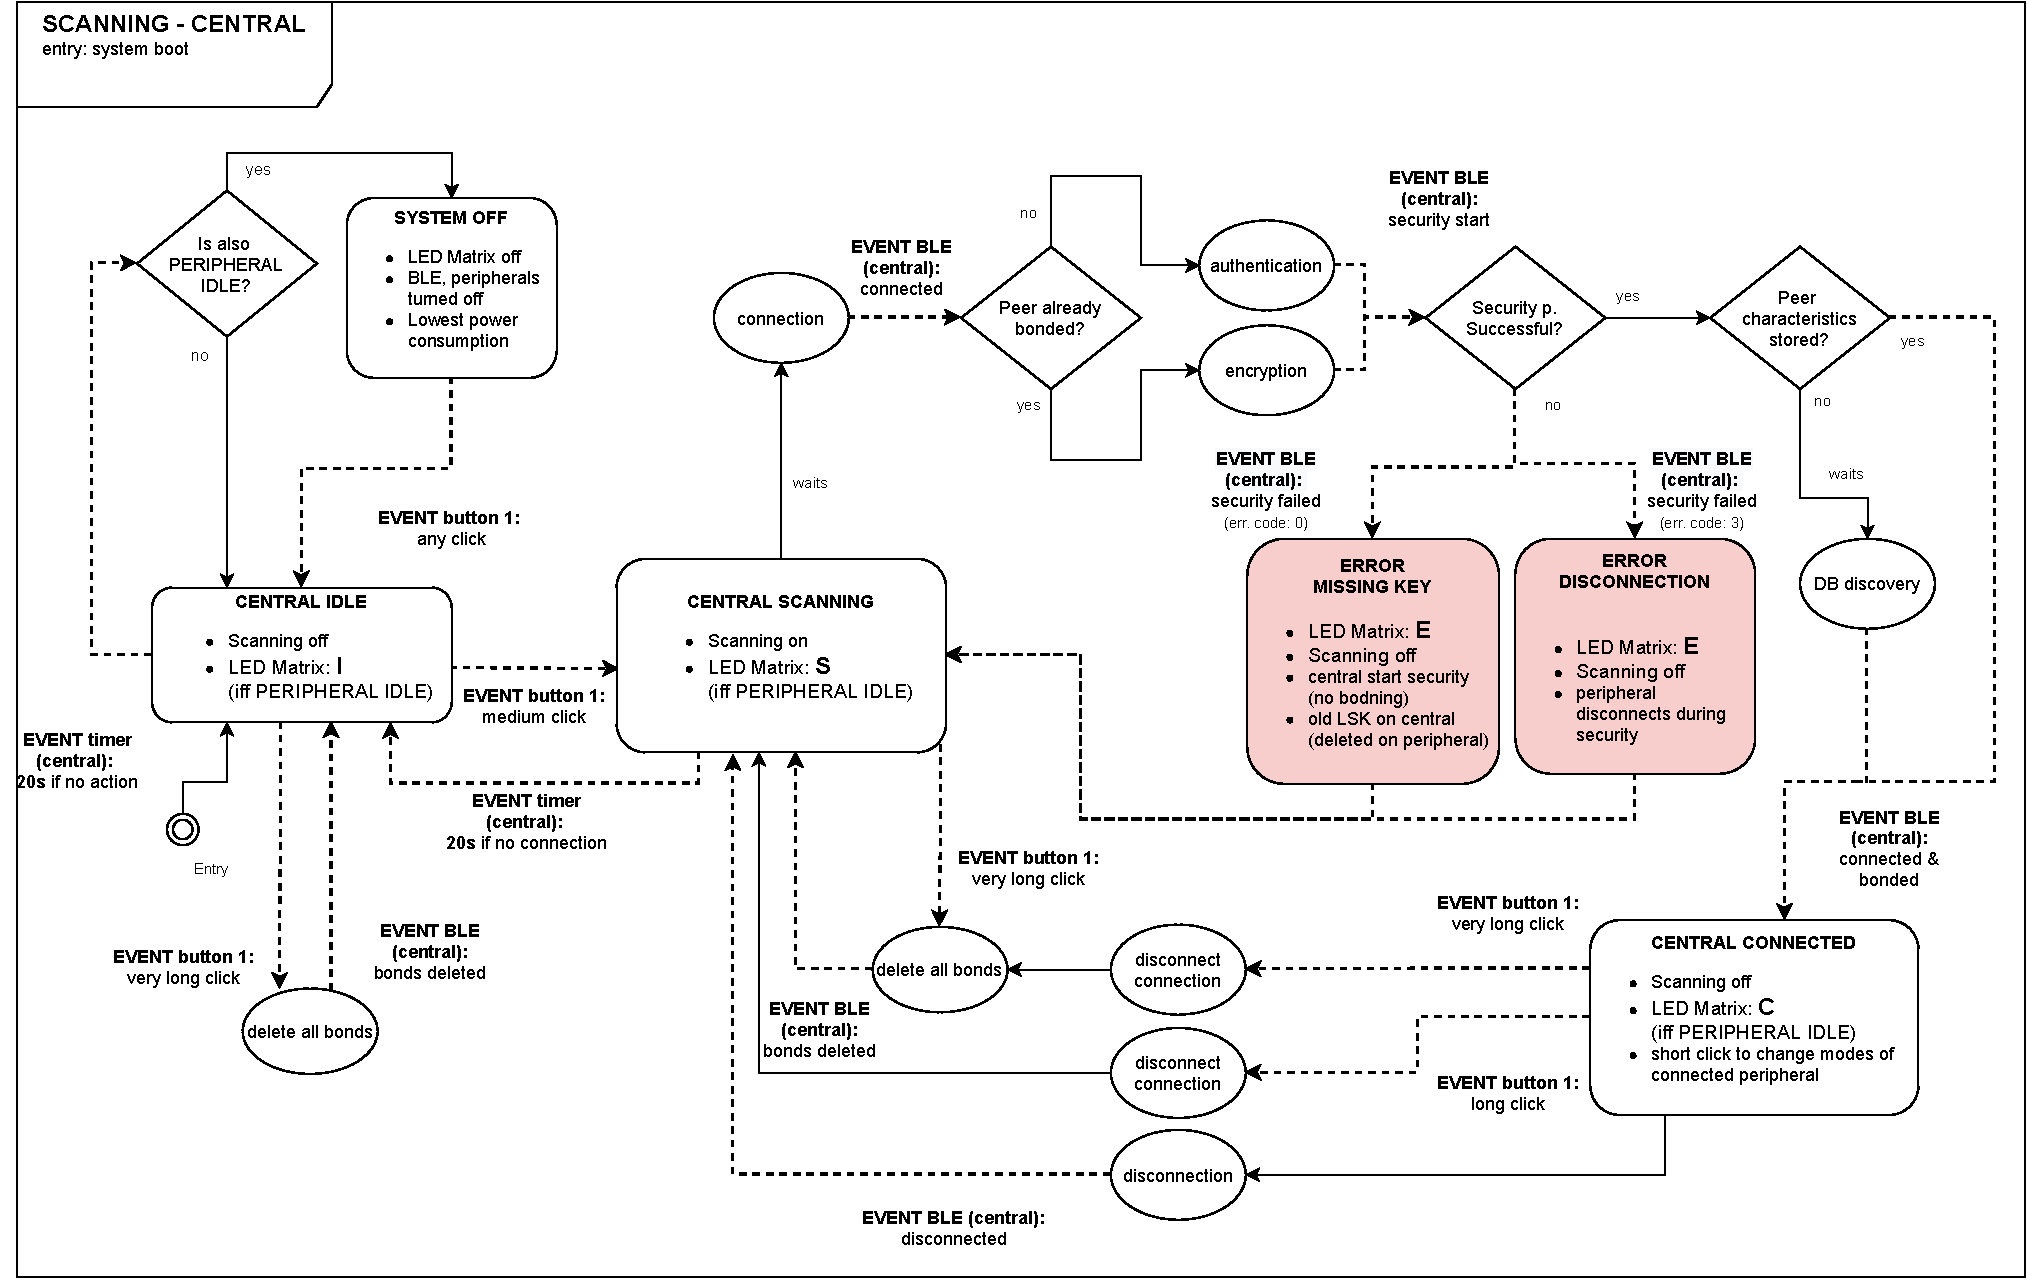
\includegraphics[ width=1.1\textwidth]{SW_Firmware/Figs/fb_scanning.pdf}
                \caption {State diagram - scanning (central)}
                \label{figure:state_diagram_fb_scanning}
            \end{figure}  
        
        \subsubsection{Central - Scanning procedure}
            \label{sec:fb_central_procedure}
            The scanning procedure is started from \sss{CENTRAL IDLE} state by the left button medium-long click. In \sss{CENTRAL} \sss{SCANNING} state the device scans for advertising packets, filtering them based on the target name. Once a light control unit is scanned, it is immediately connected and the link is either encrypted if a LTK security key exists on central or the authentication procedure is started (pairing and bonding).
            Providing that no security error occurs, the device stops scanning, the peripheral discovery procedure is started, and the \sss{CENTRAL} \sss{CONNECTED} state is entered. Otherwise, an error is indicated by the LED matrix showing the letter \textbf{E}.
            When successfully connected, the device can read or write to the \textit{LED Control Service} characteristics on the light control unit (see section \ref{sec:app_ble_services}).
            
            \textbf{Disconnection \& Deleting Bonds}\\
            In the \sss{CENTRAL} \sss{CONNECTED} state, the user is able to disconnect the current connection by a long left button click. A very long left button click deletes all bonds from flash in all states. 
        
        
            \begin{figure} [!ht]
        	    \centering
        	    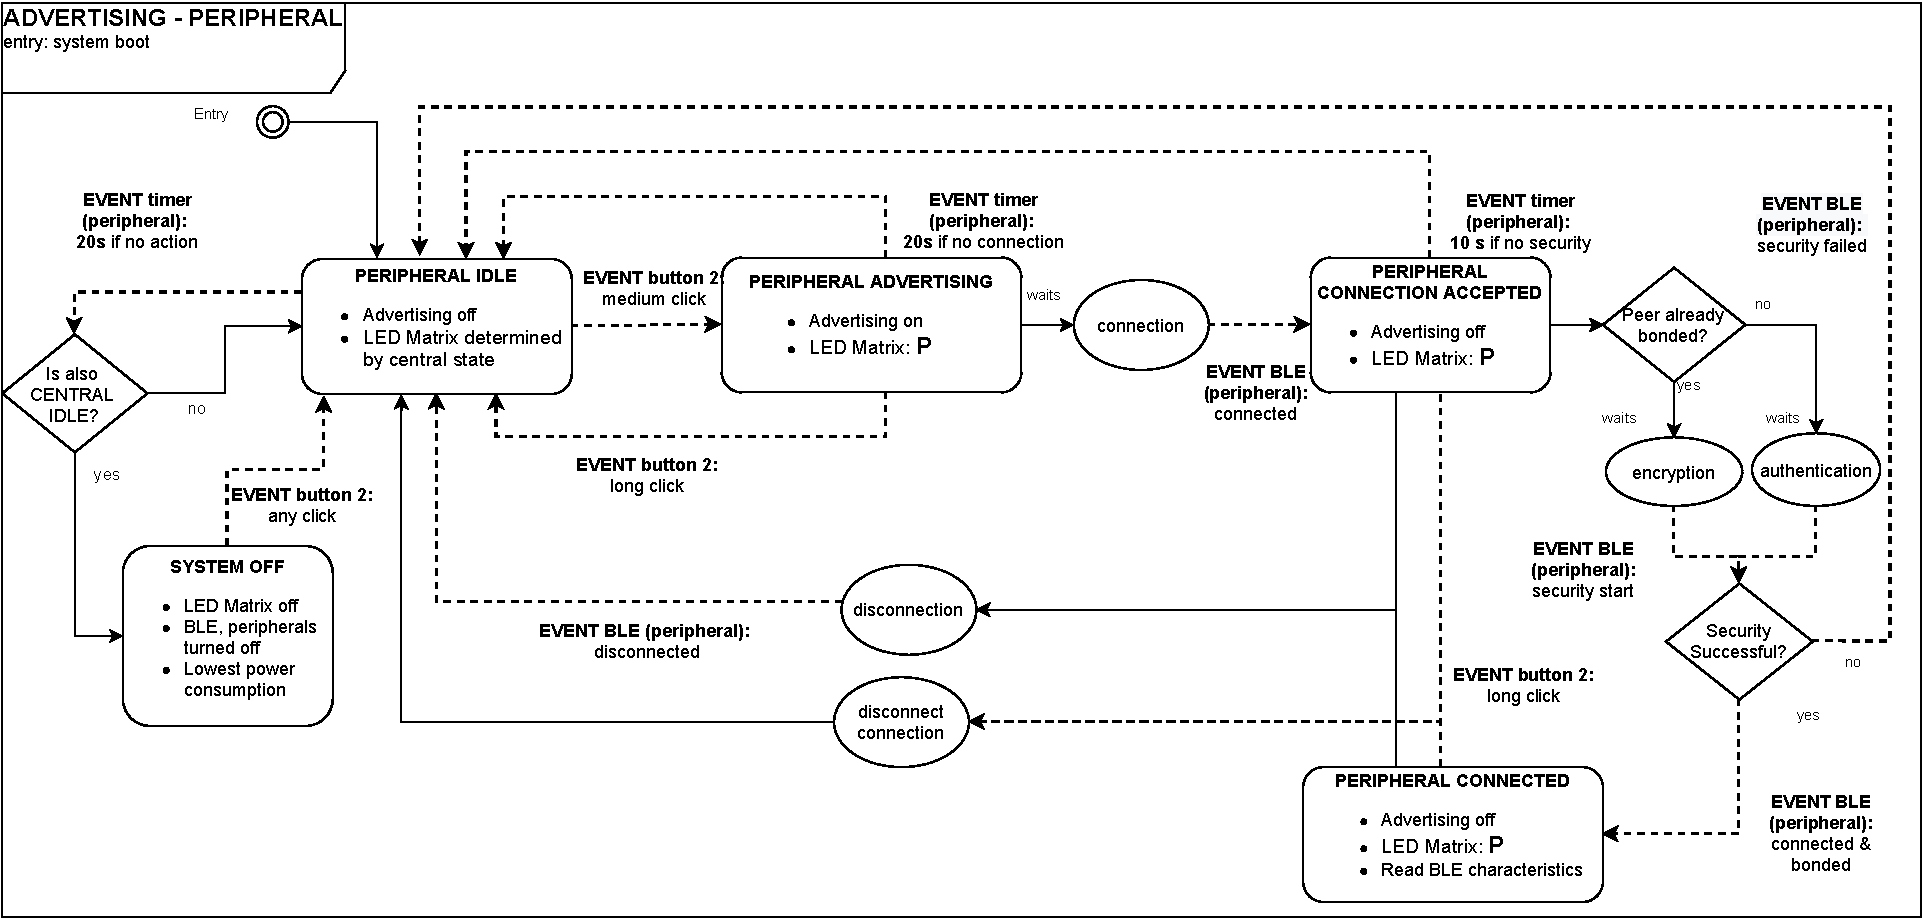
\includegraphics[ width =1.1\textwidth]{SW_Firmware/Figs/fb_advertising.pdf}
                \caption {State diagram - advertising (peripheral)}
                \label{figure:state_diagram_fb_advertising}
            \end{figure}  
        
    \subsubsection{Advertising - Peripheral Procedure}
            \label{sec:fb_peripheral_procedure}
            The \sss{PERIPHERAL} \sss{IDLE} state is the default application state for peripheral mode. A medium-long click on the right button activates the advertising to other centrals (smartphone). The peripheral mode is visualized by letter \textbf{P} on the LED matrix regardless of the current central state. Within 20 seconds, a central must connect and secure the link. While in \sss{PERIPHERAL CONNECTED} state, the characteristics from \textit{Maintenance Service} and \textit{Secure DFU Service} can be read or written.
            
            \textbf{Disconnection \& Rebooting}\\
            The long right button click disconnects the current connection (central) when in \sss{PERIPHERAL} \sss{CONNECTED} state and stops advertising in \sss{PERIPHERAL} \sss{ADVERTISING} state. In an arbitrary state, a very long right button click reboots the device. 
            
            

\section{RFID Switch}
    \label{sec:fw_rfid}
    The software techniques and algorithms used to extract data from RFID readers are introduced in this section.
    
    \subsection{Reading Data from RDM6300}
        As described in section \ref{sec:hw_rfid_rdm6300}, the RDM6300 performs all signal processing (demodulation and decoding) internally, and once the RFID tag is detected, it only transmits the received bits over UART. Because the received bytes are sent only once, the tag must be moved out from the reader's range to be transmitted again. 
        
        The 64 bits saved in the RFID tag are sent as a 14 bytes long word (see figure \ref{figure:rdm6300_word}).
        The head (first) byte of the word is always set to \textbf{0x2}, and the tail (last) byte to \textbf{0x3}. After the head, ten bytes representing the tag's unique identifier and two bytes of checksum follow. They are sent as hexadecimal characters in ASCII format..  
        
        \begin{figure} [!ht]
    	    \centering
    	    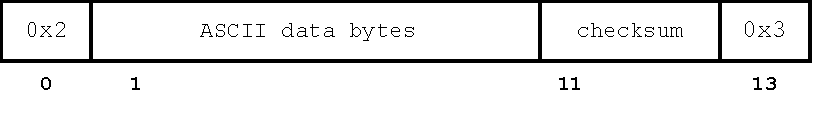
\includegraphics[ width=0.8\textwidth]{SW_Firmware/Figs/rdm6300_word.pdf}
            \caption {RDM6300 word}
            \label{figure:rdm6300_word}
        \end{figure}  
        
        The checksum is calculated as XOR operation against each pair of the data bytes converted to integer values. If the calculated checksum matches the transmitted checksum, the RFID word is valid.
        
        Upon reception of a valid RFID word, the application event \sss{EVT\_RFID\_DETECTED} is generated, and the light mode is incremented (see methods for changing light modes in section \ref{sec:light_modes_methods}).
        
        
    \subsection{Signal Processing of Custom RFID Reader}
        \todo{TO BE DONE...}
        
    
        
        
        
        
    
    
    
\section{Button Debouncing \& Press Detection}
    \label{sec:fw_buttons}
    This section aims at describing the software techniques implemented to prevent button bounces and provide press duration detection.
    
    \subsection{Button Debouncing}
        As with most mechanical switches, the basic push buttons on both boards suffer from the bouncing problem. Whenever two mechanical contacts in a button connect, they tend to bounce off each other a few times before settling down. Bouncing happens in a matter of milliseconds \cite{web_article:bouncing}. If the GPIO interrupts are used for detection, the MCU is fast enough to register all these oscillations and keep calling the interrupt handler, which might overload the MCU.
        
        An algorithm preventing bouncing uses a timer and GPIO interrupt. When an edge on the button GPIO pin occurs, three consecutive scans of the button state in 15 ms intervals are planned. The button state change is confirmed only if the pin state is the same in all three scans.
        
        In the \textbf{GPIO ISR}, the further GPIO interrupts on this pin are disabled, and a timer compare event on channel one is scheduled to scan the button state (see figure \ref{figure:btn_algorithm} showing the algorithm).\\
        Every time the \textbf{timer ISR} is called, the button state is checked at first. If the logical level of the pin is the same as the saved button state, the change is rejected, and the GPIO interrupt is enabled again. In the case of a successful third scan, the button state is changed, and the GPIO interrupt re-enabled.
        
        \begin{figure} [!ht]
    	    \centering
    	    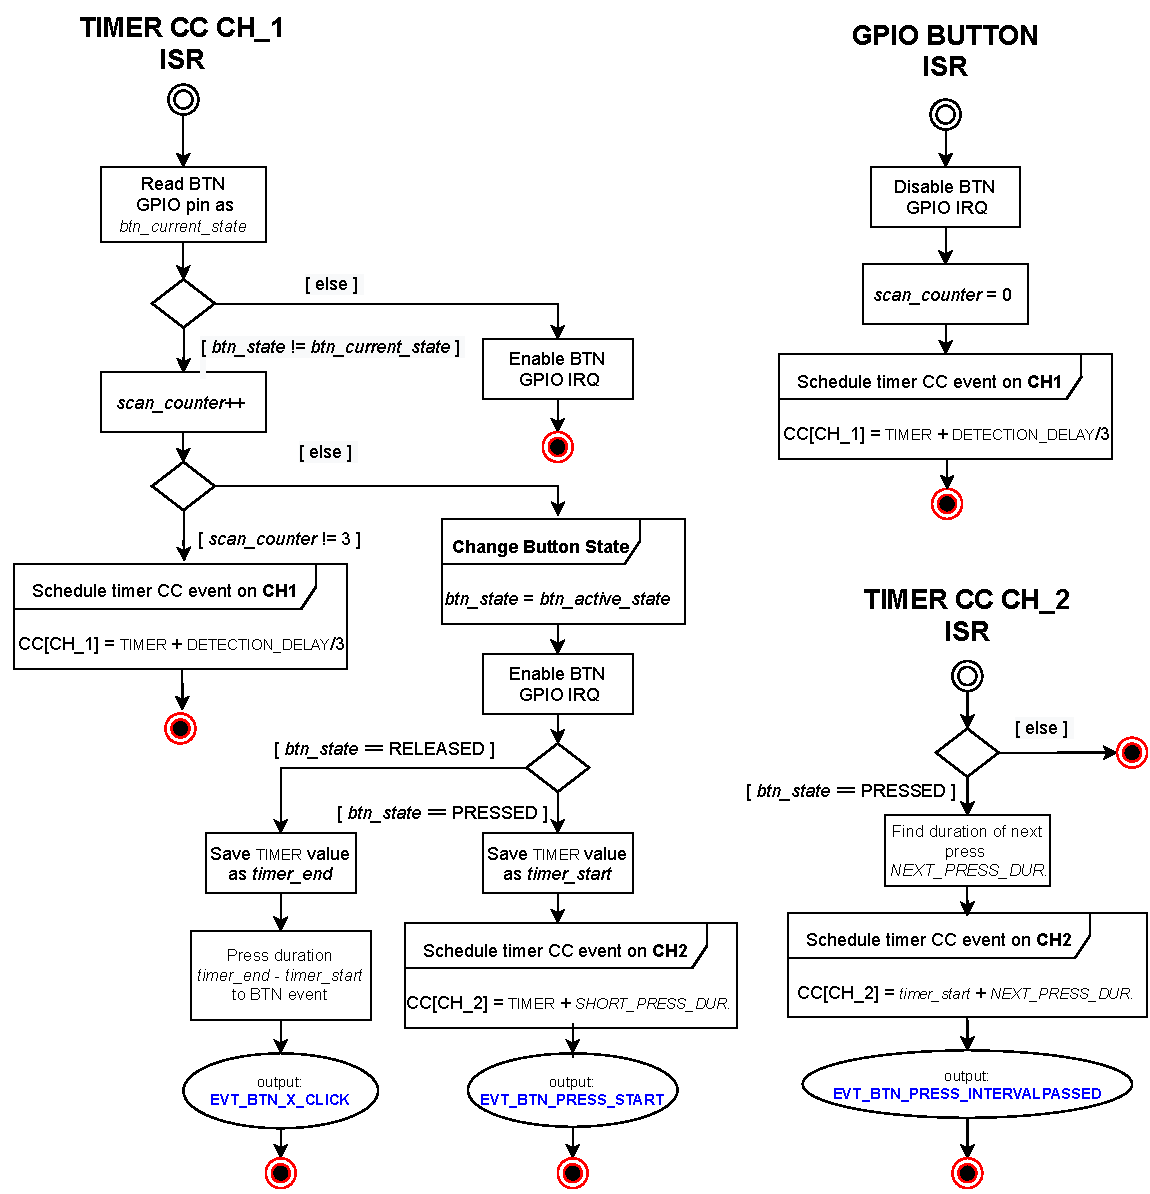
\includegraphics[ width =\textwidth]{SW_Firmware/Figs/btn_algorithm.pdf}
            \caption {Button GPIO and timer interrupt handlers (ISRs)}
            \label{figure:btn_algorithm}
        \end{figure}  
        
        One of the problems of this approach that is needed to take into account is a potential undetected button change after the read of the button state and before the GPIO interrupt is enabled. Nevertheless, this problem should be prevented by a latch register on nRF52 GPIO pins that holds the detected value, and when the interrupt is re-enabled, it immediately causes IRQ.        
    
    \subsection{Button Application Events}
        As long as the button changes its state to pressed (active), the current timer value is saved, and the application event \sss{EVT\_BTN\_PRESS\_START} is generated. Subsequently, the timer compare event on channel two is scheduled for the end of the current click interval (1000ms for a short click). Once this interrupt fires, the application event \sss{EVT\_BTN\_PRESS\_INTERVALPASSED} is outputted, and a next event scheduled.\\
        See the subsections \ref{sec:apptimer} and \ref{sec:lcu_rgb_leds} describing how are these events handled.\\
        After the button state change to released (inactive), the duration of the click is calculated based on the current timer value and the saved start time of the press. The table \ref{table:btn_click} shows the duration for particularly long clicks and the application event that is triggered.
        
        \begin{table}[!ht]
            \begin{tabular}{l!{\vrule width 1pt}c}
                \textbf{Application Event} &  \textbf{Press duration}\\ 
                \Xhline{1\arrayrulewidth}
                \sss{EVT\_BTN\_SHORT\_CLICK} & 45ms - 1s \\\hline
                \sss{EVT\_BTN\_MEDIUM\_CLICK} & 1s - 3.5s \\\hline
                \sss{EVT\_BTN\_LONG\_CLICK} &  3.5s - 8s\\\hline
                \sss{EVT\_BTN\_VERY\_LONG\_CLICK} & 8s - 20s \\
            \end{tabular}
            \caption{Button click application events and their defaul duration}
            \label{table:btn_click}
        \end{table}
        
        The logic described above is implemented in a library \verb|app_button.c|. At most, three buttons are supported (the nRF52 timer has 6 compare events).\\
    
    
\section{Battery And Temperature Measurement}
    \label{sec:fw_battery}
    This section analyzes the light control unit's battery measurement circuit and ADC configuration. The focus is also given to the estimation of battery level and the overall incorporation into the application logic.
    
    
    \subsection{Battery Measurement}
        \label{sec:battery_measurment}
        The Lithium battery has typically a voltage range of 2.7 - 4.2 V \cite{web_article:battery}. The measurement circuit consists of a voltage bridge and capacitor (see figure \ref{figure:circuit_battery}).
        
        \begin{figure} [!ht]
    	    \centering
    	    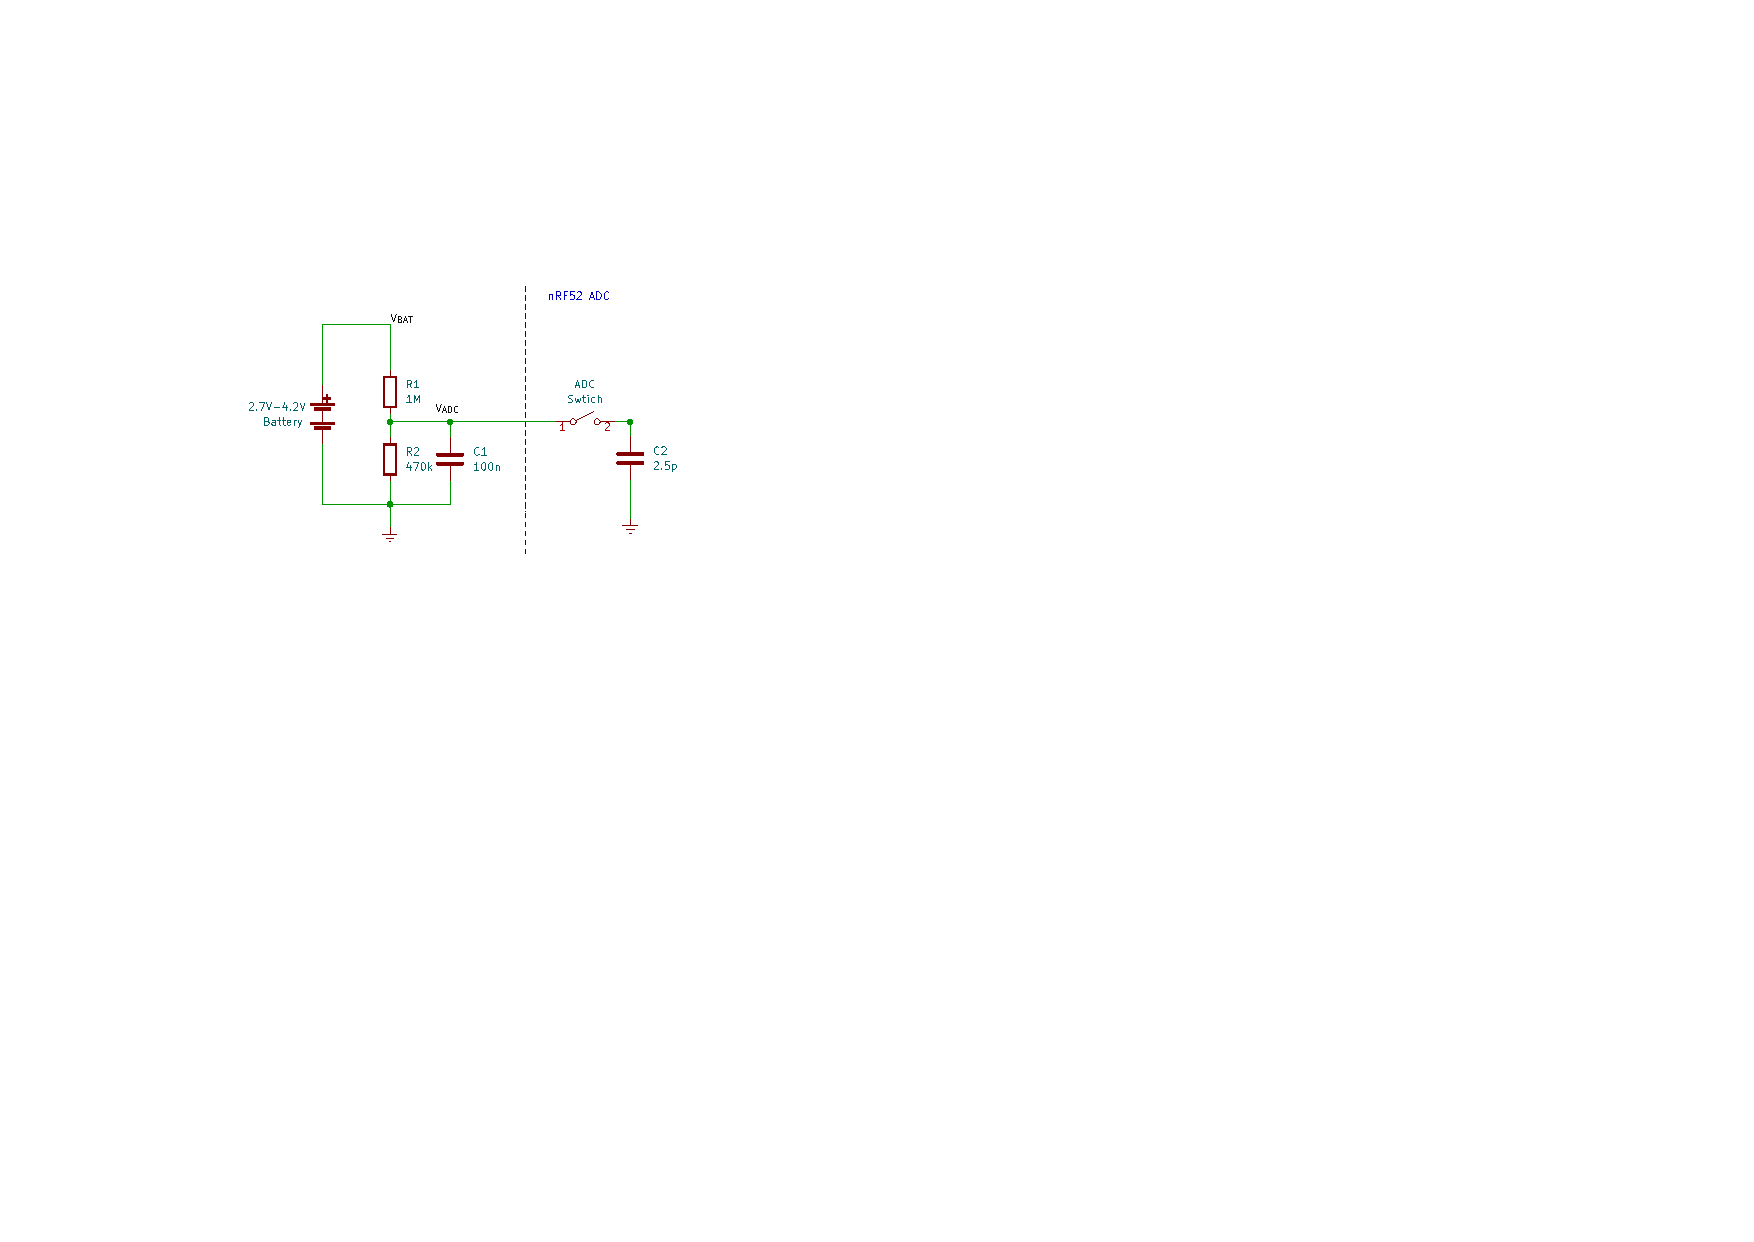
\includegraphics[width=0.9\textwidth]{SW_Firmware/Figs/battery_measurment.pdf}
            \caption {Battery measurement circuit.}
            \label{figure:circuit_battery}
        \end{figure}  
        
        \textbf{Leakage Current}\\ 
        Because the battery is connected permanently, the aim is to reduce the leakage current to the minimum, so the total resistance of the bridge should be as high as possible. According to the equation \ref{eq:adc_current}, the maximum value of the leakage current (when the battery is fully charged) is $I_{leak_{MAX}} = \SI{2.857}{\micro\ampere}$.
        
        \begin{equation}
        \label{eq:adc_current}
            I_{leak} = \frac{V_{BAT}}{R_1 + R_2}
        \end{equation}
        
         
        \textbf{Input Range}\\ 
        The internal 0.6 V reference was selected, and in accordance with the maximum possible ADC input voltage (calculated in \ref{eq:adc_min_max}), the gain  1/3 was used enabling the input voltage to go up to 1.8 V.
        
        \begin{equation}
        \label{eq:adc_min_max}\\
            V_{ADC} = V_{BAT} \, \frac{R_2}{R_1 + R_2}
        \end{equation}
        \begin{align*}
            V_{ADC_{MIN}} = \SI{863.3}{\milli\volt}\\
            V_{ADC_{MAX}} = \SI{1342.9}{\milli\volt}\\
            ADC_{MIN} = 490\\
            ADC_{MAX} = 763
        \end{align*} 
        
        
        \textbf{Acquisition time}\\ 
        Using the capacitor in the circuit has several advantages, but most importantly, it allows setting down the acquisition time to $t_{acq} = \SI{3}{\micro\second}$. Without the external capacitor, the internal ADC capacitor $C_2$ would have to be charged with a large RC time constant (due to the large value of $R_2$). Hence, a long acquisition time would be needed.\\
        The external capacitor $C_1$ is fully charged when the ADC input is disconnected. At the start of sampling, the electrical charge is distributed between external and internal capacitors proportionally to their capacities. Therefore there is a voltage drop on the external capacitor (see equation \ref{eq:voltage_drop}). The capacitor value $C_2$ should be high enough, providing the desired voltage drop is less than 1 LSB.
        
        The maximum voltage drop can be calculated assuming the battery is fully charged and the internal ADC capacitor is fully discharged:
        \begin{align}
            Q = V_{ADC_{MAX}}\, C_1 = V \, C_1 + V \, C_2\\
            \Delta V = V_{ADC_{MAX}} - V = V_{ADC_{MAX}} \, \frac{C_2}{C_1 + C_2}. \label{eq:voltage_drop}
        \end{align}
        The variable $V$ is the voltage on capacitors after the electrical charge is distributed.
        
        The value of the LSB can be calculated by knowing the maximum input voltage - $V_{RES}$ and the number of bits as follows:
        \begin{equation}
            1 \, LSB = \frac{V_{RES}}{2^n}.
        \end{equation}
        
        The resulting maximum voltage drop for selected gain and resolution is $\Delta V = \SI{3.4}{\micro\volt}$ which is less than $1\, LSB = \SI{1.8}{\milli\volt}$.
    

    
        \textbf{ADC Sampling}\\
            The battery ADC input is configured as single-ended. The measurement is done in one SAMPLE task together with other ADC channels which require larger sampling rate (around $\SI{100}{Hz}$). Only the current ADC value is saved in RAM. 
            
            The sampling is performed by PPI (\ref{sec:ppi}) independently of the MCU. The RTC COMPARE event on channel 0 triggers the ADC SAMPLE task. The RTC runs at 32.768 kHz, which gives with the prescaler of 32 and capture compare value of 10 the sampling frequency $f_s = \SI{102.4}{Hz}$. 
            
            
            \begin{equation}
                f_s = \frac{f_{RTC}}{PRES} \, \frac{1}{CC}
            \end{equation}
            
            \begin{table}[!ht]
                \begin{tabular}{l!{\vrule width 1pt}c}
                    Sampling Frequency & 102.4 Hz \\\hline
                    Resolution & 10 bit \\\hline
                    Acquisition Time $t_{acq}$ &  $\SI{3}{\micro\second}$\\\hline
                    Reference & internal 0.6 V\\\hline
                    Gain & 1/3 \\
                \end{tabular}
                \caption{ADC channel parameters for battery measurment.}
                \label{table:adc_properties}
            \end{table}
            
    \subsection{Battery Charging}
    \label{sec:battery_chargning_management}
        The battery can be charged through a USB-C connector and it is controlled by an additional chip from Microbit MCP73832-2ACI/OT, a linear charge management controller with preconditioning. This chip employs a constant-current charging if the battery voltage is below regulated voltage and a constant-voltage charging if the battery voltage is above the regulated voltage \cite{datasheet:mcp73832}.
        The constant voltage regulation is factory set (in our version to 4.2 V, corresponding to the maximum voltage of Lithium battery). The constant current value can be selected by an external programming resistor between VSS and PROG pin, and it was set to approximately 450 mA.\\
        The logical level of charge status output (STAT) pin determines whether the battery is being charged or not.
            
            
    \subsection{Temperature Measurement}
        The temperature sensor is integrated directly on the nRF52 chip. The temperature range is greater than the allowed operating temperature range of the chip and the resolution is 0.25 degree \cite[425]{datasheet:nrf52833}.
            
    \subsection{Battery Application Events}
        \label{sec:battery_estimation}
        The raw battery ADC value is read regularly triggered by the application timer. In the timer callback, the battery level is estimated, the temperature value is read, the indication is set, and BLE characteristics are updated.
        
            
        \textbf{Battery Level Estimation}\\
        Estimating the precise battery level is a complicated task. The battery discharge curve depends on the type of battery, temperature, discharge rate etc. For the sake of simplicity and according to the customer requirements, the battery levels were divided into five categories (see table \ref{table:battery_levels}). Once the battery level is measured, the application event \sss{EVT\_BATTERY\_MEASURED} is generated (see section \ref{sec:app_events} for all application events).
        
        \begin{table}[!ht]
            \begin{tabular}{l!{\vrule width 1pt}cc}
                Level 5 & 4.0 V - 4.2 V & \tikzsymbol{fill=green}\\
                Level 4 & 3.8 V - 4.0 V & \tikzsymbol{fill=yellow}\\
                Level 3 & 3.6 V - 3.8 V & \tikzsymbol{fill=purple}\\
                Level 2 & 3.4 V - 3.6 V & \tikzsymbol{fill=red}\\
                Level 1 & below 3.4 V & off \\
            \end{tabular}
            \caption{Battery levels and indication colors (on the light control unit) }
            \label{table:battery_levels}
        \end{table}
        
        On the light control unit, a particular battery level is indicated by using different colors of \textit{battery LED} (\ref{sec:lcu_rgb_leds}). On the floating button, the battery level can be obtained only through a mobile application.
        
        The LED colors corresponding to the battery levels and the frequency of the measurements is configured in \verb|app_config.h|.
         

         
        \textbf{Battery Charging Detection}\\
        Detecting whether the battery is being charged is done through GPIO interrupt for the STAT pin of the MCP73832 chip (see section \ref{sec:battery_chargning_management}). The logical level of the pin is read in the interrupt handler, and appropriate application event is generated (\sss{EVT\_BATTERY\_CHARGER\_CONNECTED} - see \ref{sec:app_events}).\\
        The application event handler then updates the BLE characteristics and sets the indication - the \textit{battery LED} is blinking if the battery is being charged.
        
        
        \textbf{Battery Damage Prevention}\\
        When the estimated battery level is below 3.4 V, the firmware automatically enters the \sss{SYSTEM OFF} mode in order to prevent the undercharging and further damaging of the battery. In this mode, the battery consumption is reduced to a minimum - all peripherals besides GPIO are turned off.
        
    
    
\section{OTA DFU} 
    \label{sec:ota}
    OTA DFU stands for Over the Air Device Firmware Upgrade referring to the fact that the DFU package with new firmware is sent to the target device wirelessly - over BLE. This section describes and explains this process and introduces its various parts.
    
    \subsection{Bootloader}
        The DFU process relies on the existence of a bootloader. The location of a bootloader and bootloader settings in memory is provided in the section \ref{sec:fw_memory_layout}. The bootloader is a minimal piece of code compiled and loaded onto the target separately from the main application. It is responsible for launching the application, entering the DFU mode or activating a new firmware \cite{nrf52doc:bootloader}.
        
        Two bootloaders, one for the light control unit and one for the floating button, were implemented - each one as a standalone project (see section \ref{sec:fw_code_structure} showing the code structure). Apart from using the different indications of DFU process steps, they are identical.
        The bootloaders implementation is based on nRF Secure Bootloader which uses security measures to protect the DFU process against malicious attackers accepting only DFU packages that are cryptographically signed with the correct key \cite{nrf52doc:secure_bootloader}.

        
    \subsection{Bootup Validation}
        \label{sec:bootup_validation}
        The bootloader checks the validity of the application every time during bootup. The CRC validation method (CRC32) is used for this purpose ensuring the data integrity of the application.\\
        The application is searched at a first bank, predefined memory address determined by the SoftDevice type (see section \ref{sec:fw_memory_layout}). Although the DFU uses dual bank update, the new firmware is always copied to the first bank after a completed and validated upgrade (check the data transfer paragraph in section \ref{sec:dfu_process}).
        
        
    \subsection{Buttonless DFU Activation}
        \label{sec:buttonless_activation}
        The DFU mode is activated by the bootloader if one of the following occurs:
        \begin{itemize}
            \item No valid application during bootup (see \ref{sec:bootup_validation})
            \item A special value present in the GPREGRET register
        \end{itemize}
        
        The GPREGRET (General Purpose REGister RETAined) is a RAM mapped retained register which preserves its value even after the system reset. In order to make the bootloader enter the DFU mode, a special reserved value must be written to this register.\\
        A connected client can turn on the DFU mode by writing to a characteristic of a vendor-specific BLE service called \textit{Secure DFU Service} (see section \ref{sec:app_ble_services}). The service then writes to the GPREGRET register and executes a system reset \cite{nrf52doc:secure_dfu_service}.

        After the device resets, the DFU mode is entered, the bootloader starts advertising with the name \textit{SunFibre - DFU}, and waits for an init packet. No authentication (bonding) procedure is required to connect and start the firmware upgrade. An inactivity timer is turned on, and if it expires, the bootloader resets back to the application. 
        
    
    \subsection{Firmware Upgrade Process}
        \label{sec:dfu_process}
        \begin{figure} [!ht]
    	    \centering
    	    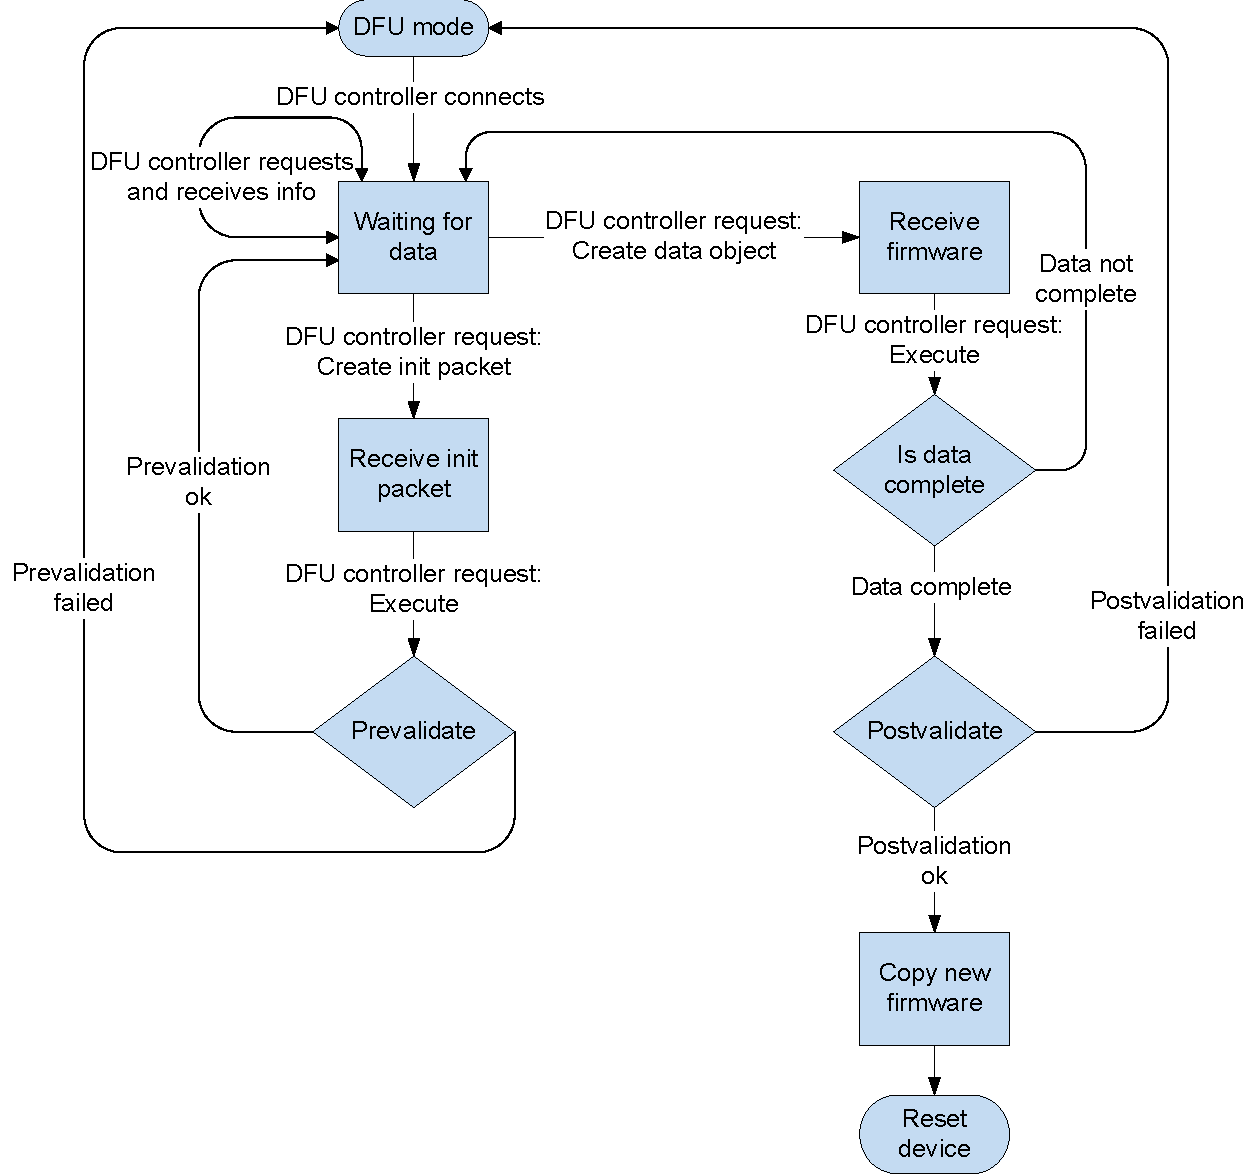
\includegraphics[width=0.9\textwidth]{SW_Firmware/Figs/nrf52_dfu.pdf}
            \caption {WorkFlow of the DFU process (taken from \cite{nrf52doc:dfu_process})}
            \label{figure:dfu}
        \end{figure}  
        
        Two devices are involved in the DFU process - the DFU controller, which transfers the DFU package (smartphone), and the DFU target (light control unit or floating button), which receives and applies the new firmware \cite{nrf52doc:dfu_process}. The whole DFU process is visualized in figure \ref{figure:dfu}.
        
        
        \textbf{Init Packet}\\ 
         At the start of the DFU process, the DFU controller transfers the init packet. It contains various fields describing the content of the DFU package (such as the type of package - in our case, the application only, hardware/firmware version, SoftDevice ID etc.). A signature generated using a private key is also added to the packet to ensure the authenticity of the firmware provider. Additionally, a hash of the whole new firmware created by the SHA256 function is appended.

        For signing the DFU upgrades, a completely new private key was generated by open-SSH.
        
        \textbf{Prevalidation}\\
        Upon successful reception of the init packet, the prevalidation is performed. At first, the signature of the DFU package is verified with the public key compiled directly in the bootloader code. Subsequently, the hardware version is checked as well as the firmware version, which prevents a possible downgrade.
        
        \textbf{Data Transfer}\\
        The DFU process is configured as a dual-bank update. The existing application is preserved until the new firmware image is activated. If the firmware update process fails, the user can still restart the device and boot the existing application.\\
        The data transfer is carried out using a BLE service on the DFU target called \textit{DFU Service}. It is a primary service with a 16-bit UUID - \textbf{0xFE59} recognized by Bluetooth SIG. The DFU controller initiates the DFU operations (init packet transfer, prevalidation, data packet transfers etc.) by writing commands to \textbf{DFU Control Point Characteristic}. A response from the DFU target comes as a BLE notification. The package is split into multiple chunks (packets) that are consecutively written to the the \textbf{DFU Packet Characteristic} and transferred \cite{nrf52doc:dfu_service}.\\
        The upgrade status is preserved in a dedicated flash memory region - MBR Params allowing the upgrade process to continue even when it was suspended (\ref{sec:fw_memory_layout}).
        
        \textbf{Postvalidation}\\
        Upon successful reception of the whole DFU package, the bootloader checks the hash of the received application image to verify the integrity of the data. If it passes, the new firmware is activated - copied from the second bank to the first bank, and the application is booted up.  
        
        
    \subsection{Tools used}
        At the time of writing, the only possible way to perform the OTA DFU is through \textit{nRFConnect} application provided by Nordic Semiconductors directly.\\
        The init packet or bootloader settings generation is possible with the help of \textit{nrfutil}, a python based command-line tool also provided by Nordic.

    
    
    
% \section{PID Regulator} 



% %!TEX ROOT=ctutest.tex
\chapter{Testování systému}
    V rámci práce byly také provedeny dva experimenty na simulátoru vibrací (obrázek \ref{figure:motor}), jež slouží pro účely předmětu Diagnostika a testování.\\
    První rotační soustava, na které byly experimenty prováděny, je tvořena stejnosměrným motorem, ložiskem bez poruchy (ložisko 2), hřídelí a poškozeným ložiskem s trhlinou na vnějším kroužku (ložisko 1). Druhá soustava s oběma ložiskami bez poruchy bohužel nebyla funkční, a nemohla tak posloužit jako reference stavu bez poškození, a proto jsme nedokázali určit, jak moc jsou vibrace způsobené trhlinou z prvního ložiska přenášeny přes hřídel na druhé ložisko.\\
    Akcelerometr byl v obou případech připevněn na ložisko tak, aby měřil vibrace v ose kolmé k ose motoru.

     \begin{figure}[!ht]
            \centering
    	    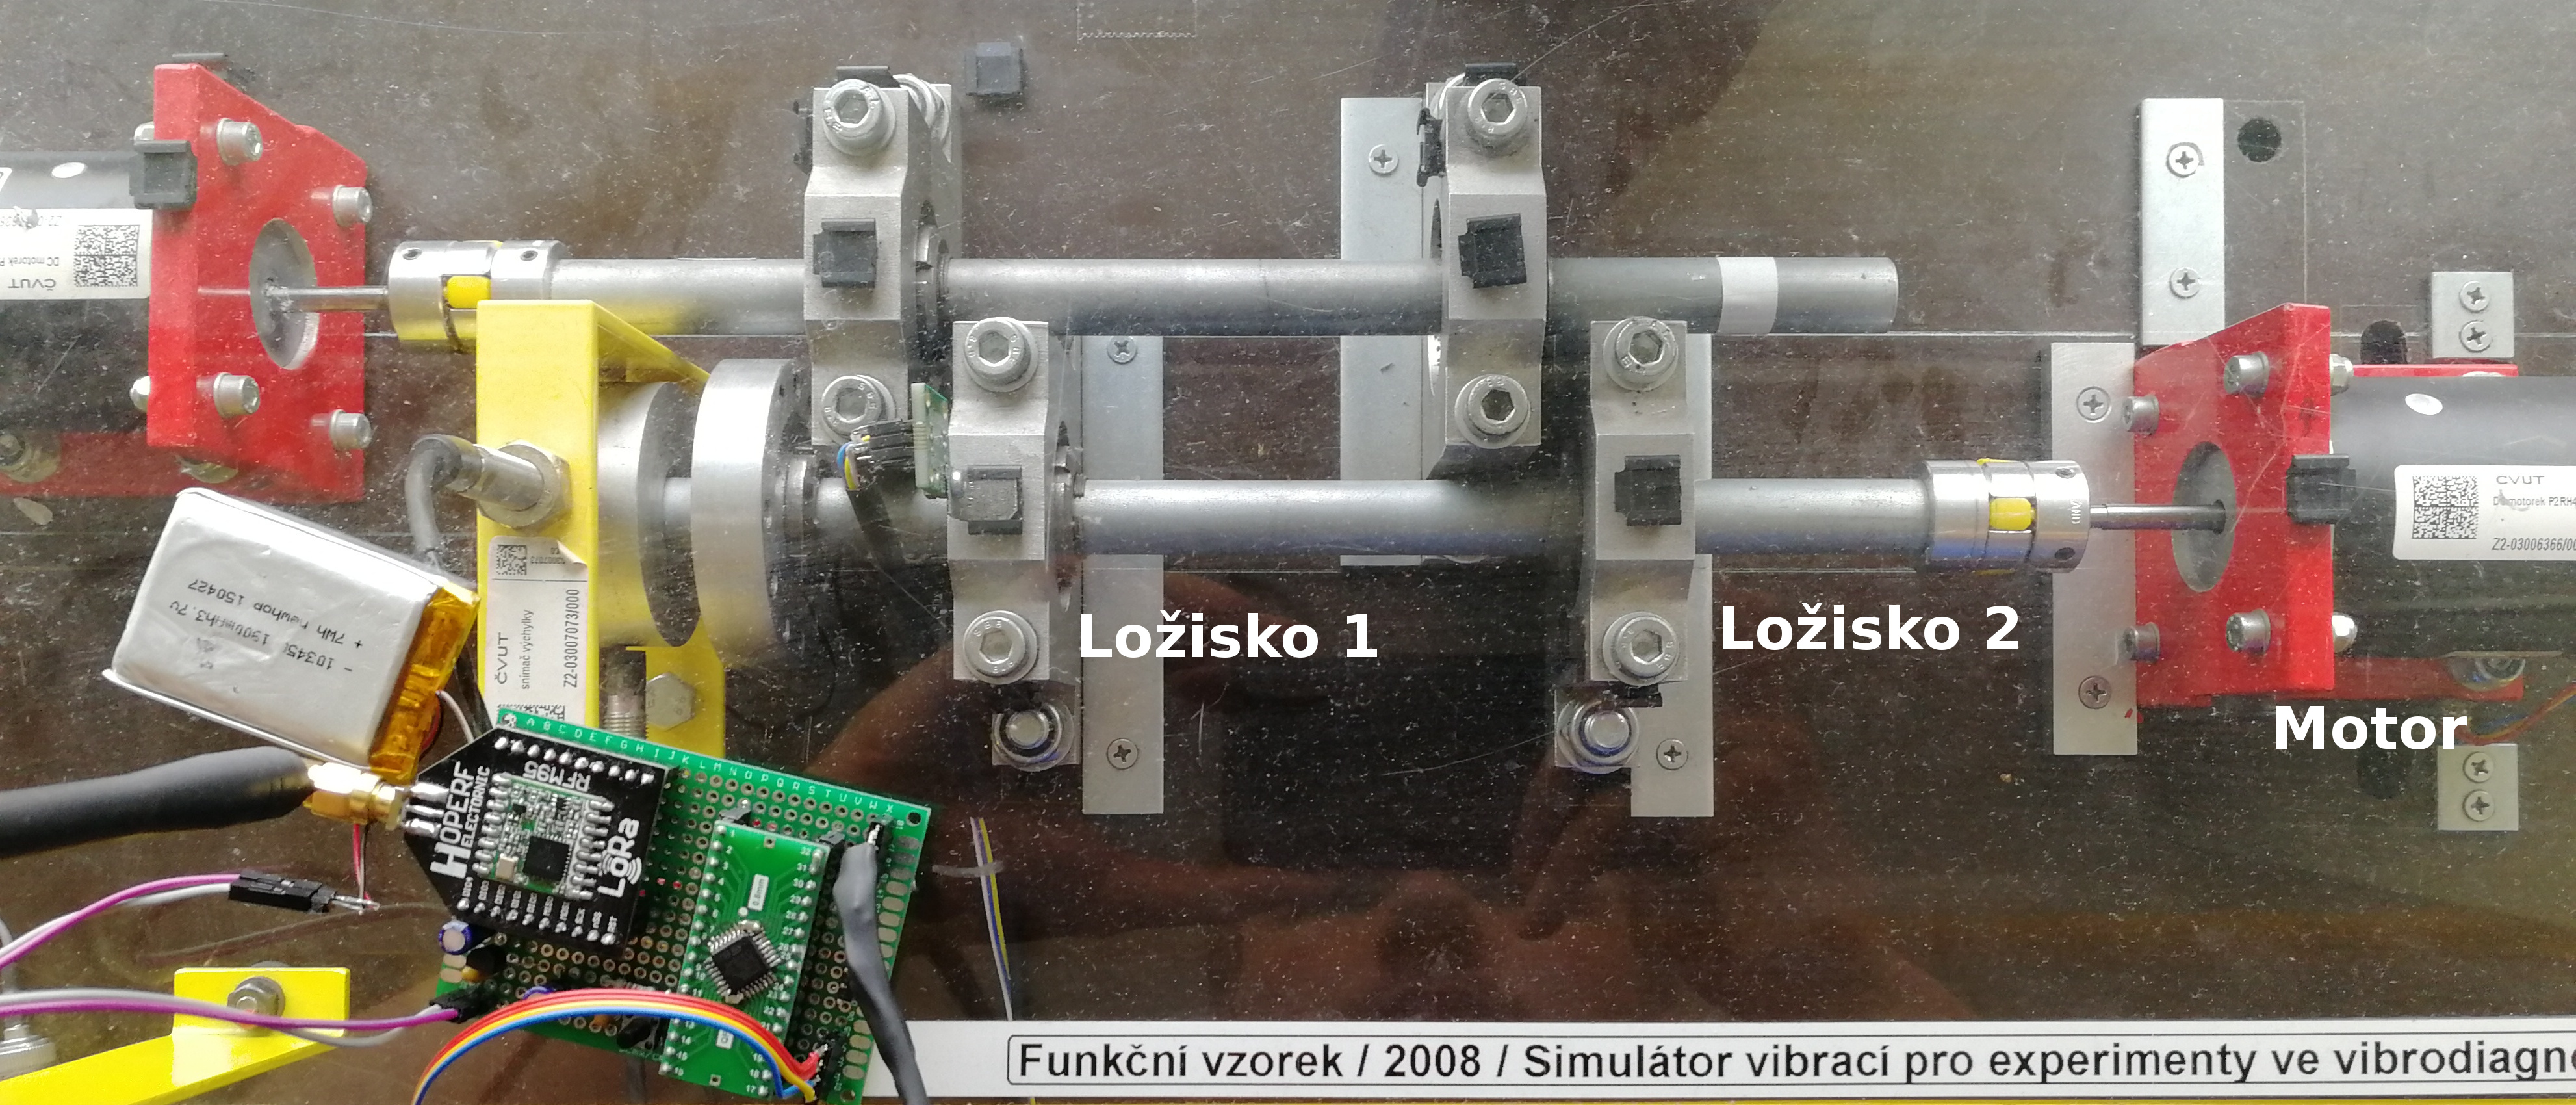
\includegraphics[width =\textwidth]{Experiment/Figs/soustava_best.jpg}
            \caption {Rotační zařízení včetně navržené měřicí jednotky.}
            \label{figure:motor}
    \end{figure}  
    \section{První experiment – nevyváženost osy}
        V prvním experimentu jsme se snažili pomocí analyzovaných příznaků detekovat nevyváženost osy, kdy byl vsazen do válcového tělesa upevněného k hřídeli nevyvážek (šroub), a způsobil tak její drobné vychylování.
        Motor byl roztočen na 3000 otáček za minutu, vzorkovací frekvence AD převodníku byla nastavena na 1.5 kHz, FFT se vypočítávalo z 1024 vzorků, data byla odesílána do centrální jednotky v desetisekundových intervalech.\\
        Nejdříve bylo druhé ložisko monitorováno bez šroubu. Následně byl systém pozastaven (lze vidět na grafech v obrázku \ref{figure:experiment_graphs01}), do kola byl vsazen šroub a v~monitorování se pokračovalo. Na závěr bylo pro případ se šroubem i bez něj v debugovacím módu aplikace odesláno celé amplitudové spektrum.
        
        \begin{figure}[!ht]
            \centering
    	    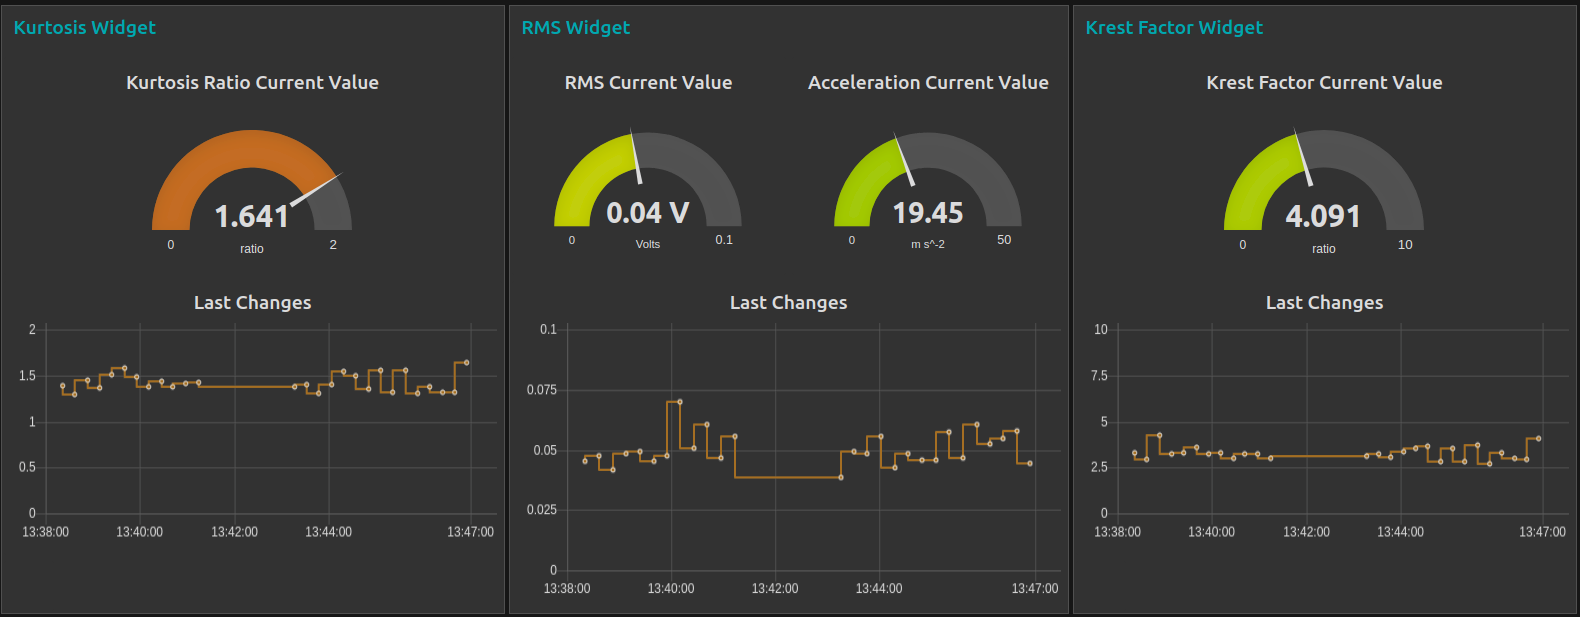
\includegraphics[width=\textwidth]{Experiment/Figs/timechanges_motor_nail.png}
            \caption {První experiment – časový průběh RMS, krest faktoru a kurtosis ratio.}
            \label{figure:experiment_graphs01}
        \end{figure}
        
        \begin{figure} [!htp]
            \centering
            \caption{První experiment – amplitudová spektra.}
            \begin{subfigure}[b]{0.48\textwidth}
                 \centering
                 \includegraphics[width=\textwidth]{Experiment/Figs/3000_rpm_1khz_ok.png}
                 \caption {Amplitudové spektrum před vsazením šroubu.}
                 \label{figure:amplitude_01}
             \end{subfigure}
             \hfill
            \begin{subfigure}[b]{0.48\textwidth}
                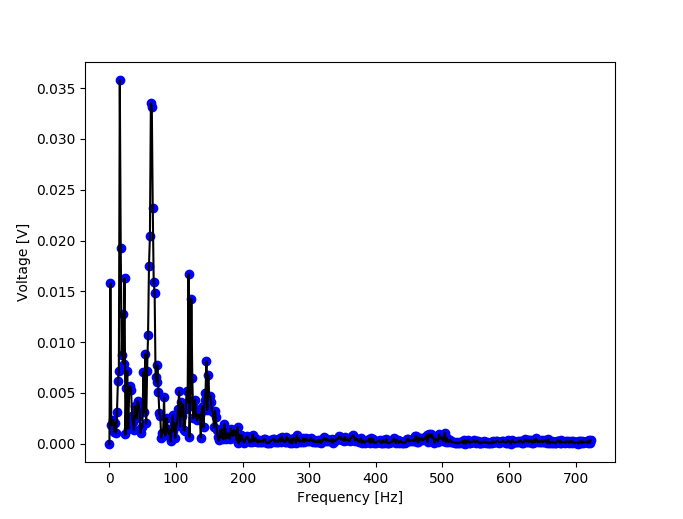
\includegraphics[width=\textwidth]{Experiment/Figs/3000_rpm_1khz_nail.png}
                \caption {Amplitudové spektrum po vsazení šroubu.}
                \label{figure:amplitude_02}
            \end{subfigure}
        \end{figure} 
    
    \subsection{Výsledky}
        Z hlediska příznaků pracujících s vibračním signálem v časové oblasti experiment ukázal, že pro přítomnost šroubu, a tím vzniklou nevyváženost osy, nejsou monitorované veličiny, krest faktor a kurtosis ratio příliš směrodatné. Hodnoty krest faktoru a kurtosis ratio spíše poskytuje informace o poruchách, které způsobují občasné impulsy s nadměrnou amplitudou (kapitoly \ref{section:kurtosis} a \ref{section:krest}).\\ 
        V amplitudovém spektru vibrací před vložením šroubu (obrázek \ref{figure:amplitude_01}) byl nejvýznamnější pík na 53 Hz, který zhruba odpovídal otáčkám motoru 3000 RPM, a 110 Hz odpovídající první harmonické frekvenci. Třetí nejvýraznější pík se nacházel na frekvenci 16 Hz a jeho původ se nepodařilo objasnit. Mohl souviset s přítomností trhliny na poškozeném ložisku nebo s vlastními rezonancemi soustavy.
        Vsazení šroubu se na amplitudovém spektru jasně projevilo, přibylo mnoho nových extrémů, které byly dokonce výraznější než původních 53 Hz (obrázek \ref{figure:amplitude_02}).\\
        Frekvenční spektrum tak opravdu podává mnohem komplexnější informace nežli časové průběhy, což potvrdilo závěry v kapitole \ref{section:techniky}.
    
            
    \section{Druhý experiment – přítomnost trhliny ve vnějším kroužku ložiska}
        V druhém experimentu jsme se snažili pomocí analyzovaných příznaků detekovat přítomnost trhliny na prvním ložisku. Trhlina způsobuje výskyt drobných impulsů v signálu, které by měly ovlivňovat hodnoty průběhů krest faktoru a kurtosis ratio.\\
        Parametry motoru a měřicí jednotky byly nastaveny stejně jako v prvním experimentu.\\
        Nejdříve bylo monitorováno první ložisko s trhlinou, poté byl systém pozastaven a akcelerometr umístěn na druhé ložisko a v~monitorování se pokračovalo. Na závěr bylo opět v obou dvou případech odesláno celé amplitudové spektrum.
        
        \begin{figure} [!hbp]
            \centering
            \caption{Druhý experiment – amplitudová spektra.}
            \begin{subfigure}[b]{0.48\textwidth}
                 \centering
                 \includegraphics[width=\textwidth]{Experiment/Figs/3000_rpm_1khz_ok.png}
                 \caption {Amplitudové spektrum nepoškozeného ložiska.}
             \end{subfigure}
             \hfill
            \begin{subfigure}[b]{0.48\textwidth}
                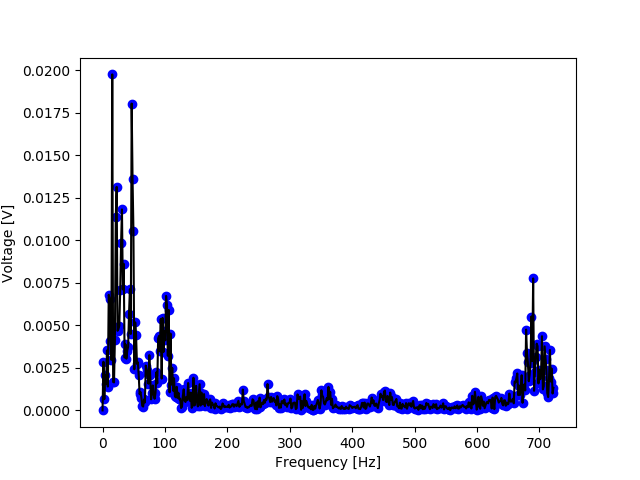
\includegraphics[width=\textwidth]{Experiment/Figs/3000_rpm_1khz_sterbina.png}
                \caption {Amplitudové spektrum ložiska s trhlinou.}
            \end{subfigure}
        \end{figure} 
        \begin{figure}[!ht]
            \centering
    	    \includegraphics[width=\textwidth]{Experiment/Figs/sterbina_300rpm_1khZ2.png}
            \caption {Druhý experiment – časové průběhy.}
            \label{figure:experiment_graphs02}
        \end{figure}
        

    
    \subsection{Výsledky}  
        Nakonec i v druhém experimentu se hodnoty kurtosis ratio a krest faktoru po přesunu akcelerometru na druhé ložisko nezměnily, i když přítomnost trhliny by pomocí nich měla být detekovatelná. Po diskusi s vedoucím práce jsme došli k závěru, že pro větší vypovídající hodnotu těchto příznaků, bychom potřebovali druhé referenční zařízení zcela bez poruchy. Dále by bylo třeba navrhnout pásmovou propust, která by vyfiltrovala signál od frekvence motoru a jejích vyšších harmonických složek, které výrazně převládají ve výpočtu, a nedovolují tak menším změnám, aby se projevily. Návrh digitálních filtrů byl ovšem nad zbylé časové možnosti.\\
        Změny se vyskytly v hodnotách RMS a ringdown counts, které se po přesunu akcelerometru na druhé ložisko zvýšily, což mělo ovšem zřejmě důvod ve větší blízkosti k motoru, a tudíž větší amplitudě vibrací, a nikoliv v přítomnosti trhliny.
        
        Amplitudové spektrum přineslo podobné výsledky jako v prvním experimentu, a i zde se tedy ukázalo jako lepší ukazatel.
        
     
        
        
% \chapter{Conclusion}
\todo{TO BE DONE...}


\appendix
% \printindex

% \chapter{Additional Picture, Schemes, Charts}
%     \begin{figure} [!h]
%     	    \centering
%     	    \includegraphics[ width =1.15\textwidth]{HW_PART/Figs/KICKAD/node.pdf}
%             \caption {Schéma zapojení monitorovací jednotky.}
%             \label{figure:scheme_01}
%     \end{figure} 
    
%     \begin{figure} [!h]
%     \label{figure:nodered_graphs}
%     	    \centering
%     	    \includegraphics[ width =1.2 \textwidth]{SW_PART/Figs/Node-RED/node_red_graphs_code.png}
%             \caption {Node-RED flowchartový program pro obsluhu grafů.}
%     \end{figure} 
    
%     \begin{sidewaysfigure}
%         \centering
%         \includegraphics[ width =\textwidth]{SW_PART/Figs/Node-RED/node_red_config_code.png}
%         \caption {Node-RED flowchartový program pro obsluhu konfigurace.}
%         \label{figure:nodered_graphs2}
%     \end{sidewaysfigure}


%     \begin{figure}[!ht]
%         \centering
% 	    \includegraphics[width =0.7\textwidth]{SW_PART/Figs/radio_packets.pdf}
%         \caption {Přehled rádiových paketů použitých v aplikaci.}
%         \label{figure:radio_packets}
%     \end{figure} 

%\appendix
\chapter*{List of Shortcuts}

\noindent
\begin{tabularx}{\linewidth}
  { l >{\raggedright\arraybackslash}X }
\bfseries Shortcut & \bfseries Meaning \\\Midrule
BLE & Bluetooth Low Energy \\
% API & Application Programming Interface \\
DMA & Direct Memory Access\\
% GPIO & General Purpose Input Output \\
% IIoT & Industrial Internet of Things\\
% IoT & Internet of Things\\
% ISM  & Industrial, Scientific and Medical\\
% $\text{I}^2\text{C}$ & Inter-Integrated Circuit\\
% LNA &Low Noise Amplifier \\
MCU & Microcontroller \\
SEPIC & Single-Ended Primary Inductor Convertor \\
RFID & Radio Frequency IDentification \\
ADC & Analog-to-Digitial Convertor \\
RAM & Randim Access Memory \\
RISC & Reduced Instruction Set Computer \\
RTC & Real Time Clock\\
SPI & Serial Peripheral Interface\\
PPI  & Programmable Peripheral Interconnect \\
UART & Universal Asynchronous Receiver/Transmitter \\
OTA & Over The Air \\
BSP & Board Support Package \\
SDK & Software Development Kit \\
ISR & Interrupt Service Routine \\
IRQ & Interrupt ReQuest\\
LSB & Least Significant Bit \\
CRC & Cyclic Redundancy Check \\
Bluetooth SIG & Bluetooth Special Interest Group\\
TTL & Transistor–Transistor Logic \\
PDU & Protocol Data Unit \\
AD & Advertising Data\\
MTU & Maximum Transmission Unit\\
LTK & Long Term Key\\ 
STK & Short Term Key\\
GAP & Generic Access Profile\\
GATT & Generic ATTribute profile\\
\end{tabularx}


% PA  & Power Amplifier \\
% PLL & Phase-Locked Loop \\
% REST & REpresentational State Transfer \\
% RMS & Root Mean Square\\
% RSSI & Received Signal Strength Indication \\
% SNR & Signal to Noise Ratio \\
% SQL & Structured Query Language \\

% TBM & Time Based Maintenance \\
% UDP & User Datagram Protocol\\
% UUID & Universally Unique IDentifier \\



\printbibliography[keyword=primary, title=Bibliography]
\printbibliography[keyword=image, title=Online Images]

% \bibliographystyle{siam}
% \bibliography{ctutest}




% \chapter{CD}




%\ctutemplate{specification.as.chapter}

\end{document}